
\chapter{Boosted VHbb Analysis}\label{chap:vhbb_boosted}

The Higgs boson, first observed by \ATLAS and \CMS at the LHC in 2012 \cite{HIGG-2012-27,CMS-HIG-12-028}, is predicted by the Standard Model to decay primarily to a pair of \bquarks, with a branching fraction of $0.582 \pm 0.007$ for $m_H = \SI{125}{\GeV}$ \cite{deFlorian:2016spz}. 
Observation of this decay mode was reported by \ATLAS \cite{HIGG-2018-04} and \CMS \cite{CMS-HIG-18-016} in 2018, establishing the first direct evidence for the Yukawa coupling of the Higgs boson to down-type quarks (see \cref{sec:higgs_yukawa_coupling}).
The \Hbb process is also important for constraining the total decay width of the Higgs \cite{Lafaye:2009vr}.

Whilst the dominant Higgs production mechanism at the LHC is gluon-gluon fusion as outlined in \cref{sec:higgs_pheno}, this mechanism has an overwhelming QCD multijet background and so overall sensitivity to the Higgs is low.
The QCD multijet background refers to events containing one or more strongly produced jets which are not the decay product of heavy resonances, for example $g \to q\bar{q}$.
In the \Hbb gluon-gluon fusion channel the vast majority of events will contain only jets in the final state, and therefore it is extremely difficult to distinguish signal events from the overwhelming multijet background.
The \hbb observation therefore searched for Higgs bosons produced in association with a vector boson $V$ (where $V$ can be a \Wboson or \Zboson boson) which subsequently decays leptonically.
The leptonic final states allow for leptonic triggering whilst at the same time significantly reducing the multijet background.

Two full \runtwo dataset analyses were carried out as a follow-up to the \Hbb observation \cite{HIGG-2018-04}.
Similar to the observation, both measured the associated production of a Higgs with a vector boson. with the Higgs boson decaying to a pair of \bquarks.
The first analysis \cite{HIGG-2018-51} was focussed on the resolved phase-space, where the Higgs candidate is reconstructed as two distinct jets with radius parameter $R = 0.4$.
The second analysis \cite{HIGG-2018-52} was focussed on the boosted phase-space, where the Higgs candidate had a sufficiently large transverse momenta such that it can be reconstructed as a single jet with a radius parameter of $R = 1.0$.
This chapter will focus on the latter analysis, which is referred to as the boosted \VHbb analysis.

In this chapter, the boosted \VHbb analysis is outlined in \cref{sec:vhbb_overview}.
An introduction to the systematic uncertainties used in the analysis is provided in \cref{sec:systematic_uncertainties}.
Detailed information about the modelling studies performed for the analysis are described in \cref{sec:vhbb_modelling}.
The statistical treatment is detailed in \cref{sec:vhbb_fit}, and the results of the analysis are presented in \cref{sec:vhbb_results}.
This analysis has been published in \rcite{HIGG-2018-52}.
Figures and tables from the published work are reproduced here.

\section{Analysis Overview}\label{sec:vhbb_overview}

The boosted \VHbb analysis is focused on the high transverse momentum regime, which has the benefit of being more sensitive to physics beyond the Standard Model \cite{Mimasu:2015nqa}, but the disadvantage of being more challenging due to the increased difficulty in the accurate reconstruction of high transverse momentum physics objects (discussed in \cref{chap:tracking}).
In order to focus on the \highpt regime, the reconstructed vector boson \ptv is required to be $\ptv > \SI{250}{\GeV}$ (see \cref{sec:vhbb_object_reco}).
Events are also split into two \pt bins with the first bin covering $\SI{250}{\GeV} < \ptv < \SI{400}{\GeV}$ and the second covering $\ptv > \SI{400}{\GeV}$, which allows the analysis to benefit from the improved signal-to-background in the \highpt regime.

The previous \ATLAS analysis in \rcite{HIGG-2018-04} was primarily sensitive to vector bosons with a more modest \ptv boost in the region of 150--\SI{300}{\GeV} (for the 0- and 1-lepton channels) and 75--\SI{300}{\GeV} (for the 2-lepton channel).
In this regime, the Higgs candidate was reconstructed using a pair of jets with radius parameter of $R = 0.4$, called \smallR jets.
However in the \highpt regime, the decay products of the Higgs boson become increasingly collimated and the \smallR jets may not be individually resolved.
In order to enhance the reconstruction of the Higgs boson candidate, this analysis uses a \largeR jet with radius parameter $R = 1.0$ to reconstruct the Higgs boson candidate.
The Higgs candidate is required to have exactly two ghost-associated and \btagged variable-radius track-jets ($b$-track-jets).
The candidate \largeR jet is reconstructed using jet substructure techniques, in particular it is trimmed by removing soft and wide-angle components, which helps to remove particles from the underlying event and pile-up collisions \cite{PERF-2012-02}.
Refer to \cref{sec:jet_reco} for more details on jet reconstruction.

On top of the binning in \ptv, selected events are further categorised into the 0-, 1- and 2-lepton channels depending on the number of charged leptons (electrons and muons) present in the reconstructed final state (also referred to as the 0L, 1L, and 2L channels respectively).
The 0-lepton channel targets the $\Zboson \higgs \rightarrow \nu\nu \bbbar$ process, the 1-lepton channel targets $\Wboson \higgs \rightarrow \ell\nu \bbbar$, and the 2-lepton channel targets $\Zboson \higgs \rightarrow \ell\ell \bbbar$, where $\ell$ is an electron or muon and $\nu$ is a neutrino.
Each channel has a dedicated set of selections which are listed in more detail in \cref{sec:vhbb_selections}.
Events in the 0- and 1-lepton channels are further split depending on the number of additional \smallR jets
not matched to the Higgs candidate.
The high-purity signal region (HP SR) has zero such jets, while the low-purity signal region (LP SR) has one or more, and therefore absorbs a larger number of background \ttbar events.
Maintaining a high purity signal region is important for the extraction of the signal yield.
%The 0- and 1-lepton channels are split into high- and low-purity signal regions based on the number of additional untagged \smallR jets present in the event.
The 0- and 1-lepton channels also make use of a dedicated \ttbar control region for jets with one or more additional \btagged \smallR jets, described in \cref{sec:vhbb_control_region}.
A complete overview of the different analysis regions is given in \cref{tab:SR_CR_definition}.

%
\begin{table}[!htbp]\small
	\footnotesize\centering
    \setlength{\tabcolsep}{0.5em} % for the horizontal padding
    \setlength{\extrarowheight}{2pt}
	\begin{tabular}{ l | c | c | c | c | c | c}
		\toprule\hline
		%\hline
		%\multirow{3}{*}{Channel}  & \multicolumn{6}{c}{Categories for both $250<p_T^V<\SI{400}{\GeV}$\ and $p_T^V \geq \SI{400}{\GeV}$} \\
		\multirow{3}{*}[-4em]{\textbf{Channel}}  & \multicolumn{6}{c}{\textbf{Analysis Regions}} \\
		\cline{2-7}  & \multicolumn{3}{c|}{$250<\ptv<\SI{400}{\GeV}$} & \multicolumn{3}{c}{$\ptv \geq \SI{400}{\GeV}$} \\
		%\cline{2-7}  & \multicolumn{2}{c}{0 add. $b$-tagged track-jets & \multicolumn{2}{c}{$\geq1$ add. $b$-tagged track-jets} & \multicolumn{2}{c}{0 add. $b$-tagged track-jets & \multicolumn{2}{c}{$\geq1$ add. $b$-tagged track-jets}\\
		\cline{2-7}  & \multicolumn{2}{c|}{\shortstack{0 add. $b$-track-jets }} & \multirow{2}{*}{\shortstack{$\geq1$ add. \\$b$-track-jets}} &  \multicolumn{2}{c|}{\shortstack{0 add. $b$-track-jets}} &  \multirow{2}{*}{\shortstack{$\geq1$ add.\\ $b$-track-jets}}\\
		
		\cline{2-3}
		\cline{5-6}
		& \shortstack{0 add. \\ small-\textit{R} jets}  & \shortstack{ $\geq1$ add.\\ small-\textit{R} jets}  &  &  \shortstack{0 add. \\ small-\textit{R} jets}  & \shortstack{$\geq1$ add. \\ small-\textit{R} jets} &  \\
		\hline\hline
		0-lepton      & HP SR  & LP SR & CR   & HP SR & LP SR  & CR   \\
		\hline
		1-lepton      & HP SR  & LP SR & CR   & HP SR & LP SR  & CR   \\
		\hline
		 2-lepton & \multicolumn{3}{c|}{SR} & \multicolumn{3}{c}{SR} \\
         \hline\bottomrule
	\end{tabular}
    \caption{Summary of the
	definitions of the different analysis regions . Signal enriched regions
	are marked with the label SR. There are regions with
	relatively large signal purity (HP SR) and with low purity (LP
	SR). Background enriched control regions are marked with the label
	CR. The shorthand ``add'' stands for additional \smallR\ jets,
	i.e. number of \smallR\ jets not matched to the Higgs-jet
	candidate.
	The medium and high \ptv regions are referred to as M\ptv and H\ptv, respectively \cite{HIGG-2018-52}. }
	\setlength{\tabcolsep}{0.5em
	}  \setlength{\extrarowheight}{1pt}
	\label{tab:SR_CR_definition}
\end{table}

%

The \largeR jet mass is used as the main discriminant in the analysis.
The signal \VHbb yields is extracted from a profile likelihood fit to the \largeR jet mass over several signal and control analysis regions, which are described in \cref{sec:vhbb_selections,sec:vhbb_control_region}.
The diboson background \VZbb yield is simultaneously extracted from the fit, and provides a cross check on the signal extraction.
The fit model (described henceforth only as ``the fit'') is described in more detail in described in \cref{sec:vhbb_fit}.







\subsection{Object Reconstruction}\label{sec:vhbb_object_reco}

The presence of neutrinos in the $\Wboson \higgs \rightarrow \ell\nu \bbbar$ and $\Zboson \higgs \rightarrow \ell\ell \bbbar$ signatures can be inferred from a momentum imbalance in the transverse plane (see \cref{sec:missing_Et}).
The vector boson transverse momentum \ptv is reconstructed as the missing transverse energy \ETmiss in the 0-lepton channel, as the magnitude of the summed \vETmiss and charged-lepton momentum in the 1-lepton channel, and as the transverse momentum of the 2-lepton system in the 2-lepton channel.

%Leptons are used for the channel classification and to select relevant events as outlined in \cref{sec:vhbb_selections}.
Electrons and muons are reconstructed and identified as outlined in \cref{sec:lepton_reco}, and following the approach described in \rcite{HIGG-2018-04}.
Leptons are required to satisfy the selections listed in \cref{tab:lepton_defs}.
\textit{Baseline} electrons are required to pass the looser likelihood-based identification selection described in \cref{sec:lepton_reco},
whilst \textit{Signal} electrons are required to satisfy a tighter likelihood identification selection.
\textit{Baseline} muons are required to pass the `loose' identification described in \rcite{PERF-2015-10}, while \textit{signal} muons are required to pass the `medium' identification working point.
All signal leptons are required to additionally satisfy a $\pt > \SI{27}{\GeV}$ selection criteria, except for muons in the 1-lepton channel where a cut of \SI{25}{\GeV} is used.
The number of baseline leptons is used to categorise the event into the 0-, 1- or 2-lepton channels.
The 1- and 2-lepton channels additionally require one signal lepton to be present.

\begin{table}[!htbp]\small
	\footnotesize\centering
    \setlength{\tabcolsep}{0.5em} % for the horizontal padding
    \setlength{\extrarowheight}{2pt}
	\begin{tabular}{ l | c | c }
		\toprule\hline
      Variable    & Electrons         & Muons \\
      \hline
      \pt         & \multicolumn{2}{c}{ $ > \SI{7}{\GeV}$} \\
      $|\eta|$    & $ < 2.47$         & $ < 2.7$ \\
      $\dzerosig$ & $ < 5$            & $ < 3$ \\
      $|\zzsth|$  & \multicolumn{2}{c}{$ < \SI{0.5}{\milli\meter}$} \\
    \hline\bottomrule
	\end{tabular}
  \caption{
    Selections applied to baseline and signal electrons and muons.
    Signal leptons are additionally required to satisfy a $\pt > \SI{27}{\GeV}$ (\SI{25}{\GeV} in the 1-lepton channel).
  }
  \setlength{\extrarowheight}{1pt}
	\label{tab:lepton_defs}
\end{table}

The analysis makes use of \largeR and variable-radius \smallR track-jets, which are described in \cref{sec:jet_reco}.
The \largeR jets are required to satisfy $\pt > \SI{250}{\GeV}$ and $|\eta| < 2.0$, and are used to reconstruct the Higgs boson candidate, while \smallR jets are used for \btagging and for selection of the analysis region.
These track-jets are required to have at least two constituent tracks with $\pt > \SI{500}{\MeV}$ and $|\eta| < 2.5$, and must themselves satisfy $\pt > \SI{10}{\GeV}$ and $|\eta| < 2.5$.
The track-jets matched to the Higgs candidate are \btagged using the MV2c10 \btagging algorithm (see \cref{chap:tracking}).
The efficiency of the tagging algorithm is calibrated to events in data \cite{PERF-2016-05,ATLAS-CONF-2018-006,ATLAS-CONF-2018-001}.
The jet tagging strategy relies on extensive studies into track-jet \btagging in boosted topologies \cite{ATL-PHYS-PUB-2014-013, PERF-2017-04}.

%The jet flavour labelling scheme is described in \cref{sec:jet_reco}.


\subsection{Event Selection}\label{sec:vhbb_selections}

An extensive list of selection cuts are applied to each event in order to reject background events whilst retaining as many signal events as possible. 
A full list of selection cuts applied to the different analysis regions is given in \cref{tab:vhbb_selection}, while some key selections are listed below.

All channels are require events with at least one \largeR jet.
The vector boson transverse momentum is also required to satisfy $\ptv > \SI{250}{\GeV}$.
The Higgs candidate is chosen as the highest \pt \largeR jet satisfying these requirements.
As mentioned, the candidate \largeR jet is required to have two ghost-associated and \btagged variable-radius track-jets.

In the 0-lepton channel, trigger selections are applied using an \ETmiss trigger with a luminosity-dependent threshold that varied between 70--\SI{110}{\GeV} depending on the data taking period.
In the 1-lepton electron sub-channel a combination of single electron triggers is used with minimum \pt thresholds between 24--\SI{26}{\GeV}.
In the muon sub-channel the same \ETmiss trigger as the 0-lepton channel is used.
Since muons are not used for the \ETmiss trigger calculations, this is in effect a \pt requirement on the muon-neutrino system, which in the analysis phase space is more efficient than a single-muon trigger.
The 2-lepton channel uses the same triggering strategy as the 1-lepton channel.
In all channels, the trigger selections applied are fully efficient for events selected using the full requirements in \cref{tab:vhbb_selection}.

The combined selections in \cref{tab:vhbb_selection} result in a signal efficiency ranging from 6--\pct{16} for the $\Wboson\higgs$ and $\Zboson\higgs$ processes depending on the channel and \ptv bin.

%
\begin{sidewaystable}[p]
    \footnotesize\centering
    \setlength{\extrarowheight}{2pt}
    \begin{tabular}{l | c|c|c|c|c|c}
      \toprule\hline
      Selection & \multicolumn{2}{c|}{0 lepton channel} & \multicolumn{2}{c|}{1 lepton channel} & \multicolumn{2}{c}{2 leptons channel} \\
      & \multicolumn{2}{c|}{} & $e$ sub-channel & $\mu$ sub-channel & $e$ sub-channel & $\mu$ sub-channel \\
      \hline
      Trigger & \multicolumn{2}{c|}{ \met } &  Single electron & \met & Single electron & \met \\
      \hline
      Leptons & \multicolumn{2}{c|}{0 \VHloose\ leptons} & \multicolumn{2}{c|}{1 \WHsignal\ lepton} & \multicolumn{2}{c}{2 \VHloose\ leptons among which} \\
      & \multicolumn{2}{c|}{ } &  $\pt>27$~GeV & $\pt>25$~GeV & \multicolumn{2}{c}{ $\geq$ 1 \WHsignal\ lepton, $\pt>27$~GeV } \\
      & \multicolumn{2}{c|}{ } &  \multicolumn{2}{c|}{no second \VHloose\ lepton}  & \multicolumn{2}{c}{both leptons of the same flavour} \\
      & \multicolumn{2}{c|}{ } &  \multicolumn{2}{c|}{ }  & - & opposite sign muons  \\
      
      \hline
      \met & \multicolumn{2}{c|}{ $> 250$ GeV} & $> 50$ GeV & -  & \multicolumn{2}{c}{-} \\
      \hline
      \pTV & \multicolumn{6}{c}{$\pTV > 250$ GeV } \\
      \hline
      %Jets & \multicolumn{6}{c}{ at least one large-\textit{R} jet} \\
      %\hline
      %Large-R jet \pt & \multicolumn{6}{c}{ > 250 GeV} \\
      \LargeR jets & \multicolumn{6}{c}{ at least one large-\textit{R} jet, $\pt> 250$ GeV, $|\eta| < 2.0$} \\
      \hline
      Track-jets & \multicolumn{6}{c}{at least two track-jets, $\pt > 10$ GeV,  $|\eta| < 2.5$, matched to the leading large-\textit{R} jet} \\
      \hline
      $b$-tagged jets & \multicolumn{6}{c}{leading two track-jets matched to the leading large-\textit{R} must be $b$-tagged (MV2c10, 70\%)} \\
      \hline
      \mJ      & \multicolumn{6}{c}{$> 50$ GeV} \\
      \hline
      $\min[\Delta \phi$(\vecmet, \smallR\ jets)] & \multicolumn{2}{c|}{ $> 30^{\circ}$} & \multicolumn{4}{c}{-} \\
      \hline
      $\Delta \phi$(\vecmet, $H_{\text{cand}}$) & \multicolumn{2}{c|}{ $> 120^{\circ}$} & \multicolumn{4}{c}{-} \\
      \hline
      $\Delta \phi$ (\vecmet, \vecmpt) & \multicolumn{2}{c|}{ $< 90^{\circ}$} & \multicolumn{4}{c}{-} \\
      \hline
      $\Delta y (V, H_{\text{cand}})$ & \multicolumn{2}{c|}{-} & \multicolumn{4}{c}{$|\Delta y (V, H_{\text{cand}})| < 1.4$} \\
      \hline
      \mll & \multicolumn{4}{c|}{-} & \multicolumn{2}{c}{ 66 GeV $< \mll < 116$ GeV} \\
      \hline
      Lepton \pT imbalance & \multicolumn{4}{c|}{-} & \multicolumn{2}{c}{$(\pT^{\ell_{1}} - \pT^{\ell_{2}} ) / \pTZ < 0.8$} \\
   %   \hline
  %    Lepton flavour & \multicolumn{4}{c|}{-} & \multicolumn{2}{c}{two leptons of the same flavour} \\
   %   \hline
    %  Lepton charge & \multicolumn{4}{c|}{-} & &opposite \\
    %  			 & \multicolumn{4}{c|}{-} & & sign muons \\
  
  %    \pTV regions & \multicolumn{6}{c}{250 GeV < \pTV < 400 GeV  and \pTV > 400 GeV } \\
  %    \hline
  %    \hline
  %    \multirow{2}{*}{Signal regions} & \multicolumn{4}{c|}{ 0 add. small-R jets, > 1 add. small-R jets } & \multicolumn{2}{c}{\multirow{2}{*}{-}} \\
  %    \cline{2-5}
  %    & \multicolumn{4}{c|}{ 0 add. \btagged track-jets} & \multicolumn{2}{c}{}\\
  %    \hline
  %    \hline
  %    Control regions &  \multicolumn{4}{c|}{> 1 add. \btagged track-jets} &  \multicolumn{2}{c}{ - } \\
      \hline\bottomrule
    \end{tabular}
    \caption{
        Event selection requirements for the boosted $VH$, \Hbb analysis channels and sub-channels \cite{HIGG-2018-52}.
        Various channel dependent selections are used to maximise the signal efficiency and reduce the number of background events in each analysis region.
    }
    \label{tab:vhbb_selection}
\end{sidewaystable}
  
%

\subsection{Control Regions}\label{sec:vhbb_control_region}

% the 0L ttbar etmiss can come from W->lv, mostly where the lepton is a hadronic tau or a low pT electron/muon which are out of acceptance or not reconstructed (plus the b-jet could be lost somehow)

The \ttbar process presents a major background in the 0- and 1-lepton channels.
In these events, the Higgs candidate is often reconstructed from a correctly tagged \bjet from the top decay $t \to \Wboson b$, and an incorrectly tagged $c$- or \ljet from the subsequent decay of the \Wboson, as shown in \cref{fig:sr_cr_diagrams}.

The top quark decays to a \Wboson and a \bquark the vast majority of the time.
Hence, the second top quark from the \ttbar pair is also likely to result in a second tagged \btagged track-jet outside of the \largeR Higgs candidate.
To ensure sufficient \ttbar rejection, 0- and 1-lepton channel signal regions are defined using a veto on events with \btagged track-jets outside the Higgs candidate.
These events are used to construct a control region (CR) which is enriched in \ttbar events.
The CR is used to constrain the normalisation of the \ttbar background in the fit.

%
\begin{figure}[!htbp]
  \centering
  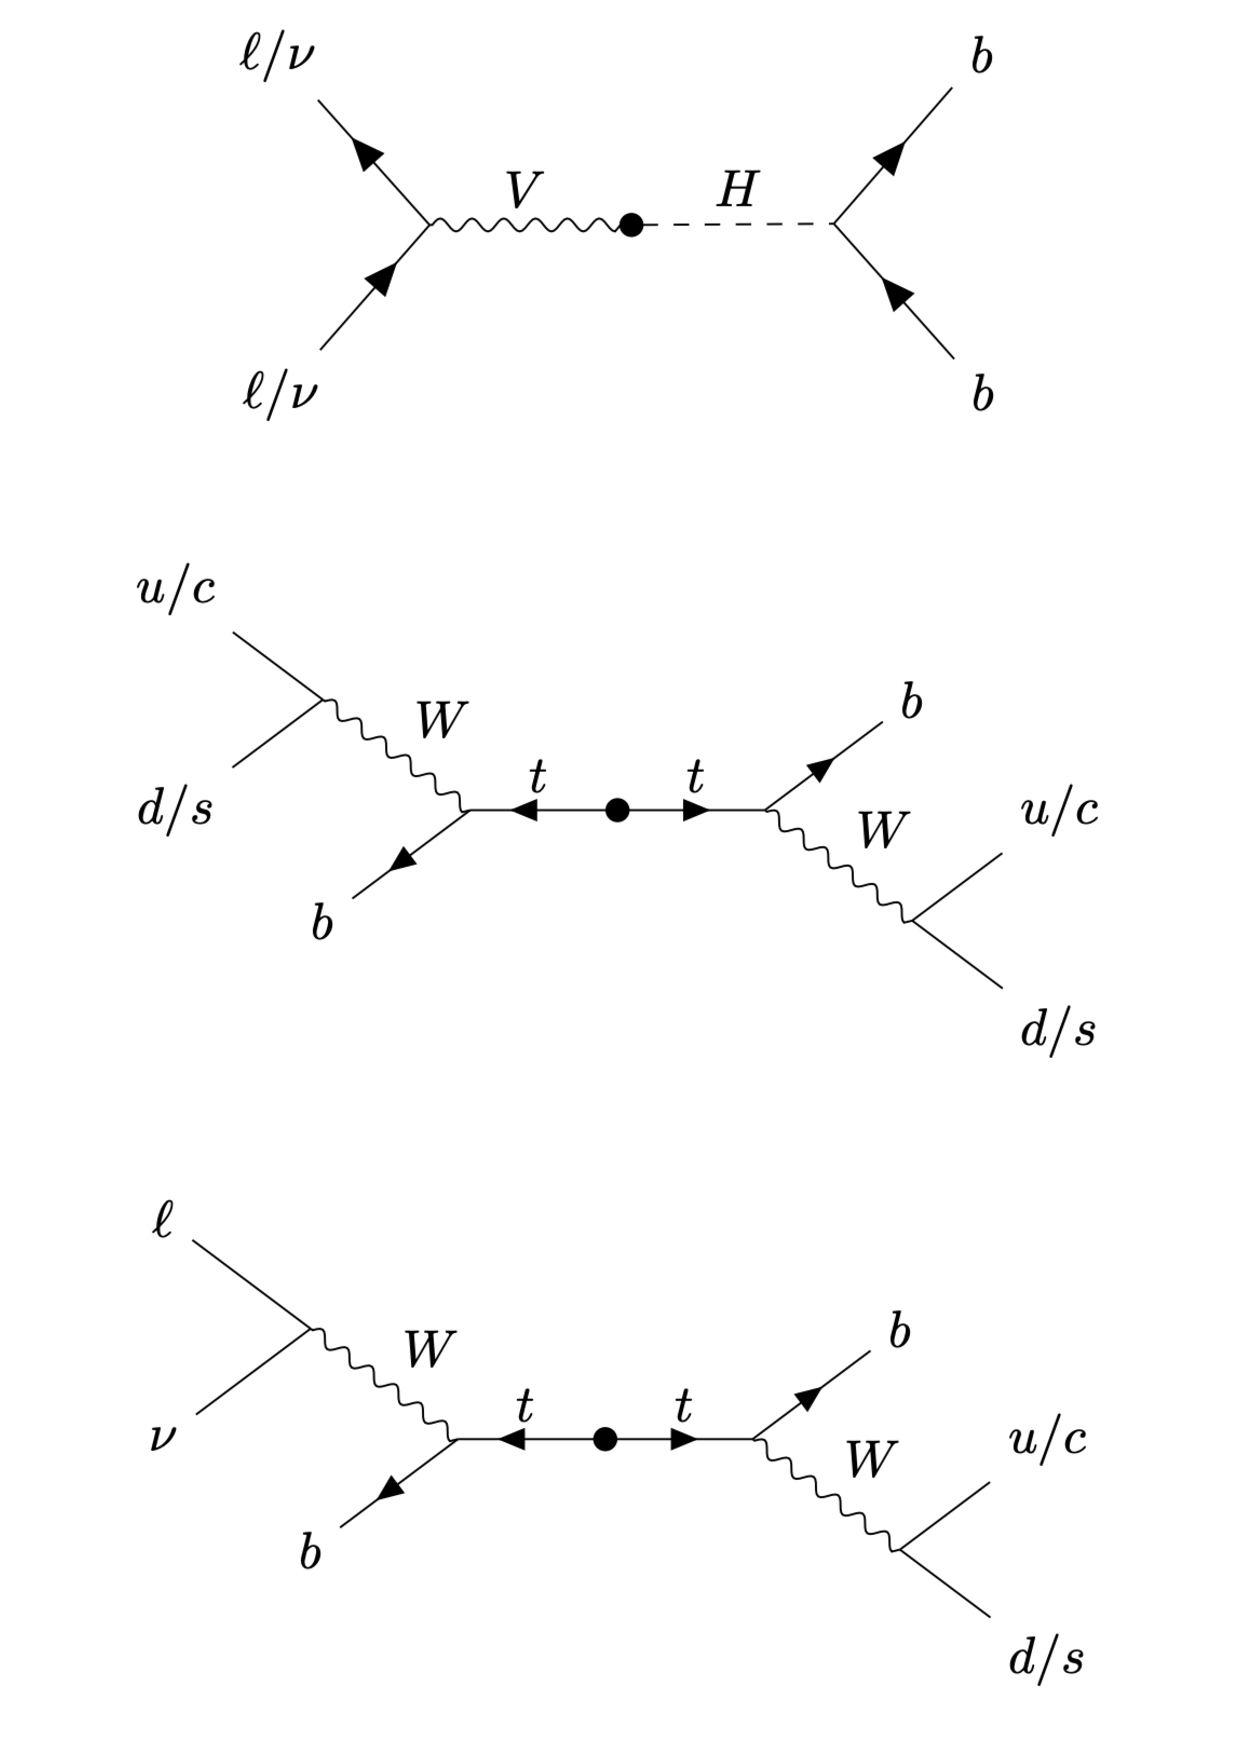
\includegraphics[width=0.65\textwidth]{chapters/6.vhbb_boosted/figs/sr_cr_diagrams.pdf}
  \caption{
    Diagrams of the signal process (top) and \ttbar background (bottom).
    The object to the right of centre are reconstructed within the \largeR jet.
    For the \ttbar background, the \largeR jet contains a mistagged $c$-jet or (less often) a mistagged \ljet.
    The contribution in the 0-lepton channel results from hadronically decaying $\tau$ lepton, or a electron or muon which is out of the analysis acceptance.
    For the \ttbar background process to be in the signal region, the \bjet on the left hand side must either be not within acceptance, not reconstructed, or not tagged.
  }
  \label{fig:sr_cr_diagrams}
\end{figure}
%

\subsection{Background Composition}\label{sec:vebb_background_composition}

After the selections described in \cref{sec:vhbb_selections} the number of background events mimicking the \VHbb signal is greatly reduced.
However, the number of background events still greatly outnumbers that of signal events.
The background processes are channel dependent.
In the 0-lepton channel the dominant sources of backgrounds are \Zjets ($\Zboson \to \nu\nu$) and \ttbar, with \Wjets and diboson events being subdominant.
\Wjets contribute in the event of $\Wboson \to \tau\nu$, and subsequent hadronic decay of the $\tau$ or lack of successful reconstruction/selection of the leptonic decay products.
\ttbar and \Wjets (with a leptonic decay of the \Wboson as in $\Wboson \to \ell\nu$) are dominant in the 1-lepton channel, while single-top is subdominant.
In the 2-lepton channel, \Zjets ($\Zboson \to \ell\ell$) is again dominant followed by $ZZ$ diboson events.

The diboson background $VV$ consists primarily of $WZ$ and $ZZ$ events in which the \Zboson decays to a pair of \bquarks.
This process very closely matches the signal, with a resonant peak occurring at $m_Z = \SI{91}{\GeV}$.
As it is a well understood process, the diboson background can be used as a cross-check on the Higgs results.

The $t\overline{t} V$, $t\overline{t} H$ and multijet backgrounds are negligible in the analysis phase space after the selections have been applied, with the exception of the 1-lepton electron sub-channel, in which multijet background is not negligible.
The multijet background in this region is generally made up of events where the isolated leptonic signature has been mimicked by either a jet or electron from a semi-leptonic heavy flavour decay, where the electron has escaped the jet.
%jets with semileptonic heavy-flavour-hadron decays (e.g. $b \to c \ell \nu$) and jets which are mistagged by the flavour tagging algorithm MV2c10.

The contributions from the different backgrounds are modelled using Monte Carlo event generators and the uncertainties associated with these samples are studied in \cref{sec:vhbb_modelling}.
The multijet background is modelled using a data-driven technique.


\subsection{Data \& Simulated Samples}\label{sec:vhbb_samples}

Data from centre-of-mass energy \come{13} proton-proton collisions at the \LHC recorded over the course of \runtwo (between 2015 and
2018) were used for the analysis.
The resulting dataset corresponds to a total integrated luminosity of \intlumi.

An overview of the MC simulated samples used in the analysis is given in \cref{tab:vhbb_samples}.
These samples are used to model the signal and background processes relevant to the analysis, with the exception of the multijet background which is modelled using a data-driven technique.
Data and simulated events are reconstructed using the same algorithms, and a reweighting is applied to the simulated events in order to match the pile-up distribution
observed in the data.
%
\begin{table}[tb!]
    \begin{center}{\fontsize{7}{7.9}\selectfont
    \begin{tabular}{llllll} 
      \toprule
    Process & ME generator & ME PDF &PS and & UE model & Cross-section \hspace{2.5cm}\\
    & & & Hadronisation & tune & order\\ 
    \toprule
    \multicolumn{6}{l}{Signal ($m_H = 125$~GeV and $b\bar{b}$ branching fraction set to 58\%)} \\
    \midrule
     $qq\to WH\to\ell\nu b\bar{b}$  &\textsc{Powheg-Box v2}~\cite{Alioli:2010xd} +&
    NNPDF3.0NLO$^{(\star)}$~\cite{Ball:2014uwa} &\PYTHIAV{8.212}~\cite{Sjostrand:2014zea} & AZNLO~\cite{Aad:2014xaa} & NNLO(QCD)+  \\
            &   \textsc{GoSam}~\cite{Cullen:2011ac} + \textsc{MiNLO}~\cite{Hamilton:2012np,Luisoni:2013kna}  & & & &NLO(EW)~\cite{Ciccolini:2003jy,Brein:2003wg,Ferrera:2011bk,Brein:2011vx,Ferrera:2013yga,Ferrera:2014lca,Campbell:2016jau} \\
    $qq\to ZH\to\nu\nu b\bar{b}/\ell\ell b\bar{b}$ &\textsc{Powheg-Box v2} + & NNPDF3.0NLO$^{(\star)}$ &\PYTHIAV{8.212} & AZNLO & NNLO(QCD)$^{(\dagger)}$+  \\
            &   \textsc{GoSam} + \textsc{MiNLO}  & & & &NLO(EW) \\
    $gg  \to ZH\to\nu\nu b\bar{b}/\ell\ell b\bar{b}$ &\textsc{Powheg-Box v2} & NNPDF3.0NLO$^{(\star)}$ &\PYTHIAV{8.212} & AZNLO & NLO+  \\
            &  & & & &NLL~\cite{Altenkamp:2012sx,Hespel:2015zea,Harlander:2014wda,Harlander:2013mla,Brein:2012ne}\\
    \midrule
    \multicolumn{6}{l}{Top quark ($m_t = 172.5$~\GeV)}  \\
    \midrule
    $t\bar{t}$ &\textsc{Powheg-Box v2}~\cite{Alioli:2010xd,Frixione:2007nw} &  NNPDF3.0NLO &\PYTHIAV{8.230} &A14~\cite{ATL-PHYS-PUB-2014-021}& NNLO+NNLL~\cite{Czakon:2011xx} \\
    $s$-channel &\textsc{Powheg-Box v2}~\cite{Alioli:2009je,Alioli:2010xd} & NNPDF3.0NLO &\PYTHIAV{8.230} &A14 & NLO~\cite{Kidonakis:2010tc} \\
    $t$-channel &\textsc{Powheg-Box v2}~\cite{Alioli:2009je,Alioli:2010xd} & NNPDF3.0NLO &\PYTHIAV{8.230} &A14& NLO~\cite{Kidonakis:2011wy} \\
    $Wt$ &\textsc{Powheg-Box v2}~\cite{Re:2010bp,Alioli:2010xd} & NNPDF3.0NLO &\PYTHIAV{8.230} &A14& Approximate NNLO~\cite{Kidonakis:2010ux} \\
    \midrule
    \multicolumn{6}{l}{Vector boson + jets} \\
    \midrule
    $W\to\ell\nu$ & \textsc{Sherpa 2.2.1}~\cite{Gleisberg:2008ta,Bothmann:2019yzt,Cascioli:2011va,Gleisberg:2008fv} & NNPDF3.0NNLO &  \textsc{Sherpa 2.2.1}~\cite{Schumann:2007mg,Hoeche:2012yf} & Default & NNLO~\cite{Catani:2009sm}  \\
    $Z/\gamma^{*}\to\ell\ell$ & \textsc{Sherpa 2.2.1} & NNPDF3.0NNLO &  \textsc{Sherpa 2.2.1} & Default & NNLO    \\
    $Z\to\nu\nu$ & \textsc{Sherpa 2.2.1} & NNPDF3.0NNLO &  \textsc{Sherpa 2.2.1} & Default & NNLO    \\
    \midrule
    \multicolumn{6}{l}{Diboson} \\
    \midrule
    $qq \to WW$ & \textsc{Sherpa 2.2.1} & NNPDF3.0NNLO &  \textsc{Sherpa 2.2.1} & Default & NLO  \\
    $qq \to WZ$ & \textsc{Sherpa 2.2.1} & NNPDF3.0NNLO &  \textsc{Sherpa 2.2.1} & Default & NLO  \\
    $qq \to ZZ$ & \textsc{Sherpa 2.2.1} & NNPDF3.0NNLO &  \textsc{Sherpa 2.2.1} & Default & NLO  \\
    $gg \to VV$ & \textsc{Sherpa 2.2.2} & NNPDF3.0NNLO &  \textsc{Sherpa 2.2.2} & Default & NLO  \\
    \bottomrule
    \end{tabular}}
    %\begin{tabular}{llllll} 
    %  \toprule
    %\hspace*{0.3cm} Process & ME generator & ME PDF &PS and & UE model & Cross-section \hspace{2.5cm}\\
    %& & & Hadronisation & tune & order\\ 
    %\midrule
    %\multicolumn{6}{l}{Signal ($m_H = 125$~GeV)\ and $b\bar{b}$ branching fraction to 58\%} \\
    % \midrule
    %\hspace*{0.3cm} $qq\ensuremath{\rightarrow} WH$  &\textsc{Powheg-Box v2}~[69] +&
    %NNPDF3.0NLO$^{(\star)}$~[70] &\PYTHIAV{8.212}~[61] & AZNLO~[71] & NNLO(QCD)+  \\
    %\hspace*{0.5cm} $\ensuremath{\rightarrow}\ell\nu b\bar{b}$&   \textsc{GoSam}~[72] + \textsc{MiNLO}~[73,74]  & & & &NLO(EW)~[75--81] \\
    %\hspace*{0.3cm} $qq\ensuremath{\rightarrow} ZH$ &\textsc{Powheg-Box v2} + & NNPDF3.0NLO$^{(\star)}$ &\PYTHIAV{8.212} & AZNLO & NNLO(QCD)$^{(\dagger)}$+  \\
    %\hspace*{0.5cm}$\ensuremath{\rightarrow}\nu\nu b\bar{b}/\ell\ell b\bar{b}$&   \textsc{GoSam} + \textsc{MiNLO}  & & & &NLO(EW) \\
    %\hspace*{0.3cm} $gg  \ensuremath{\rightarrow} ZH$ &\textsc{Powheg-Box v2} & NNPDF3.0NLO$^{(\star)}$ &\PYTHIAV{8.212} & AZNLO & NLO+  \\
    %\hspace*{0.5cm}$\ensuremath{\rightarrow}\nu\nu b\bar{b}/\ell\ell b\bar{b}$&  & & & &NLL~[82--86]\\
    %\midrule
    %\multicolumn{6}{l}{Top quark, mass set to 172.5~GeV}  \\
    %\midrule
    %\hspace*{0.3cm} $t\bar{t}$ &\textsc{Powheg-Box v2}~[87] &  NNPDF3.0NLO &\PYTHIAV{8.230} &A14~[88]& NNLO+NNLL~[89] \\
    %\hspace*{0.3cm} $s$-channel &\textsc{Powheg-Box v2}~[90] & NNPDF3.0NLO &\PYTHIAV{8.230} &A14 & NLO~[91] \\
    %\hspace*{0.3cm} $t$-channel &\textsc{Powheg-Box v2}~[90] & NNPDF3.0NLO &\PYTHIAV{8.230} &A14& NLO~[92] \\
    %\hspace*{0.3cm} $Wt$ &\textsc{Powheg-Box v2}~[93] & NNPDF3.0NLO &\PYTHIAV{8.230} &A14& Approximate NNLO~[94] \\
    %\midrule
    %\multicolumn{6}{l}{Vector boson + jets} \\
    %\midrule
    %\hspace*{0.3cm} $W\ensuremath{\rightarrow}\ell\nu$ & \textsc{Sherpa 2.2.1}~[64, 95, 96] & NNPDF3.0NNLO &  \textsc{Sherpa 2.2.1}~[97, 98] & Default & NNLO~[99]  \\
    %\hspace*{0.3cm} $Z/\gamma^{*}\ensuremath{\rightarrow}\ell\ell$ & \textsc{Sherpa 2.2.1} & NNPDF3.0NNLO &  \textsc{Sherpa 2.2.1} & Default & NNLO    \\
    %\hspace*{0.3cm} $Z\ensuremath{\rightarrow}\nu\nu$ & \textsc{Sherpa 2.2.1} & NNPDF3.0NNLO &  \textsc{Sherpa 2.2.1} & Default & NNLO    \\
    %\midrule
    %\multicolumn{6}{l}{Diboson} \\
    %\midrule
    %\hspace*{0.3cm} $qq \ensuremath{\rightarrow} WW$ & \textsc{Sherpa 2.2.1} & NNPDF3.0NNLO &  \textsc{Sherpa 2.2.1} & Default & NLO  \\
    %\hspace*{0.3cm} $qq \ensuremath{\rightarrow} WZ$ & \textsc{Sherpa 2.2.1} & NNPDF3.0NNLO &  \textsc{Sherpa 2.2.1} & Default & NLO  \\
    %\hspace*{0.3cm} $qq \ensuremath{\rightarrow} ZZ$ & \textsc{Sherpa 2.2.1} & NNPDF3.0NNLO &  \textsc{Sherpa 2.2.1} & Default & NLO  \\
    %\hspace*{0.3cm} $gg \ensuremath{\rightarrow} VV$ & \textsc{Sherpa 2.2.2} & NNPDF3.0NNLO &  \textsc{Sherpa 2.2.2} & Default & NLO  \\
    %\bottomrule
    %\end{tabular}}
    \caption
    {
      %The generators used for the simulation of the signal and background
      %processes. 
      Signal and background processes with the corresponding generators used for the nominal samples. 
      If not specified, the order of the cross-section
      calculation refers to the expansion in the strong coupling constant
      ($\alphas$).  $(\star)$ The
      events were generated using the first PDF in the NNPDF3.0NLO set and
      subsequently reweighted to the PDF4LHC15NLO
      set~\cite{Butterworth:2015oua} using the internal algorithm in
      \textsc{Powheg-Box v2}.  $(\dagger)$ The NNLO(QCD)+NLO(EW)
      cross-section calculation for the $pp \to ZH$ process already
      includes the $gg\to ZH$ contribution.  The $qq\to ZH$ process is
      normalised using the cross-section for the $pp \to ZH$ process,
      after subtracting the $gg\to ZH$ contribution. An additional scale
      factor is applied to the $qq \rightarrow VH$ processes as a function
      of the transverse momentum of the vector boson, to account for
      electroweak (EW) corrections at NLO\@. This makes use of the $VH$
      differential cross-section computed with
      \textsc{Hawk}~\cite{Denner:2011id,Denner:2014cla}.
      \protect}
    \label{tab:vhbb_samples}
    \end{center}
\end{table}
    
%

\subsection{Overview of Systematic Uncertainties}\label{sec:systematic_uncertainties}

Systemic uncertainties are extensively employed to reflect assumptions and inaccuracies in the various inputs used by the fit.
Two main types of systematic uncertainty are considered: experimental and modelling.
%Theoretical uncertainties arise due to imperfect precision used in e.g. QCD calculations.
Experimental uncertainties arise due to the imperfect modelling of the reconstruction algorithms (in particular the jet reconstruction and \btagging algorithms), and due to the imperfect modelling of pile-up and other effects, as described in \cref{sec:experimental_uncertainties}.
Modelling uncertainties arise due to the imperfections in the Monte-Carlo generators used to model the signal and background events.
In order to observe a certain process, for example \VHbb, an increase in the number of observed events with respect to the background-only hypothesis is looked for.
The excess is often relatively small against the total number of background events, and hence accurate modelling of the expected number of background and signal events is crucial for successfully performing the analysis.


\section{Experimental Uncertainties}\label{sec:experimental_uncertainties}

The main experimental uncertainties in the analysis are due to the modelling of following sources:

\begin{itemize}
  \item The \smallR jet energy scale and resolution, which are informed by in situ calibration studies \cite{PERF-2016-04}.
  \item The \largeR jet energy and mass scales and resolutions. The scales are calibrated as described in \rcite{JETM-2018-02}, and an uncertainty of \pct{2} and \pct{20} is applied for the jet energy and mass resolutions, respectively.
  \item \btagging uncertainties, which are computed separately for \bcl flavour jets as described in the data-based calibration studies in Refs.~\cite{PERF-2016-05,ATLAS-CONF-2018-006,ATLAS-CONF-2018-001}. An additional extrapolation uncertainty is added to account for jets with transverse momenta above that which is accessible in the calibration analyses.
  \item Uncertainties associated with the lepton energy and momentum scales, and reconstruction and identification efficiencies.
  \item Uncertainty on the pile-up models which are used in the simulated samples, described in \rcite{STDM-2015-05}.
  \item Uncertainties associated with the reconstruction of the missing transverse energy \ETmiss, as described in \rcite{PERF-2016-07}.
  \item Uncertainty on the total recorded integrated luminosity, as described in \rcite{ATLAS-CONF-2019-021}.
\end{itemize}

The impact of these uncertainties on the analysis can be found in \cref{tab:mu_syst_unc}.



\section{Background Modelling}\label{sec:vhbb_modelling}
% modelling note \cite{Bell:2316951}

Particular care is paid to the uncertainties on the modelling predictions as discussed in the following sections.
The \textit{Nominal} MC samples are used as a reference to which different variations can be compared.
The nominal samples are chosen as the best possible representation of the underlying physical process.
\textit{Alternative} samples are used to understand inaccuracies that may be present in the nominal samples.
Some aspect of the nominal model is varied, and the discrepancy with respect to the nominal model is quantified.
The discrepancy is used to estimate a systematic uncertainty associated with the model parameter which was varied.
The alternate samples are sometimes obtained via internal weight variations or parameterisation methods, rather than by re-running the simulation.
This is discussed in more detail in \cref{sec:implementation_of_variations}.

Modelling systematics can have several impacts, including affecting the overall normalisation for different processes, the relative acceptances between different analysis regions (i.e. migrations between HP and LP SRs, between the SR and CR, and between \pTV bins), and the shapes of the \mJ distributions.
For each source of uncertainty, acceptance and shape uncertainties are therefore derived.
Acceptance uncertainties account for the uncertainty in the overall number of events in each channel, and for the relative numbers of events in the various analysis regions.
Meanwhile, shape uncertainties account for the uncertainty on the kinematic distributions of the events, but not overall normalisations.
They are measured for the shape of the \largeR jet mass distribution, since this is the variable used in the fit to data.

In this section, truth tagging, the method used to ensure sufficient numbers of jets are available to calculate uncertainties, is described in \cref{sec:truth_tagging}.
The different sources of background modelling uncertainty which have been assessed are described in \cref{sec:sources_of_uncertainties}, and details of their implementations are found in \cref{sec:implementation_of_variations}.
Full descriptions of the modelling uncertainties applied for the \Vjets and diboson backgrounds are given in \cref{sec:vjets_modelling} and \cref{sec:diboson_modelling}, respectively.


\subsection{Truth Tagging}\label{sec:truth_tagging}

Modelling studies involving $c$- and \ljets is hampered by the low number of events available after the analysis selection is applied, due to the high rejection rates of the \btagging algorithm MV2c10.
For modelling studies, truth tagging (TT) is therefore employed to ensure sufficient numbers of jets are available to calculate uncertainties.
TT works by computing a 2-dimensional efficiency map using the jet \pt and $\eta$.
The two leading track-jets associated to the \largeR jet are weighted based on their probability to pass the \btagging selection, rather than being required to explicitly pass the \btagging requirement.
The probability to pass the \btagging selection is parameterised by the jet \pt and $\eta$, and is extracted using a pre-calculated efficiency map.

\subsection{Sources of Systematic Modelling Uncertainties}\label{sec:sources_of_uncertainties}

This section briefly describes the different sources of uncertainty in the analysis, and how each is implemented.

\subsubsection{QCD Scales}
\begin{comment}
Perturbative QCD predictions for inelastic pp scattering depend on two scales that arise
when dealing with UV and IR divergences: renormalization scale μR and factorization scale μF
The choice of these scales is arbitrary, to get a feeling for the dependence, the scales are
by convention varied usually by a factor 2 in both directions
\end{comment}
The \Vjets matrix element calculations contains infrared and ultraviolet divergences.
These are handled by introducing arbitrary parameters corresponding to the renomalisation scale ($\mu_R$) and factorisation scale ($\mu_F$).
Physical observables are not dependent on these parameters when using the infinite perturbation series expansion, however at some fixed order in QCD a limited is present.
To assess the impact of this, both $\mu_R$ and $\mu_F$ are independently varied from their nominal values by factors of $0.5$ and $2$ to account for higher order corrections to the calculation of the matrix element used to simulate the process.

\subsubsection{PDF Sets}

Parton distribution functions (PDFs) specify the probability of finding a parton with a given momentum inside a hadron (in this case, colliding protons).
PDFs have to be derived from data and are a significant source of uncertainty in analyses of hadronic collision data.
There are three sources of PDF uncertainties: the statistical and systematic errors on the underlying data used to derive the PDFs, the theory which is used to describe them (which is based on some fixed order perturbative QCD expansion), and finally the procedure which is used to extract the PDFs from the data. 
PDF-related uncertainties were derived following \rcite{Butterworth:2015oua}.
This involves considering 100 PDF replicas which, when combined, form a central value and associated uncertainty, and also in parallel direct changes to the central values of PDFs using the MMHT2014 \cite{Harland-Lang:2014zoa} and CT14NLO \cite{Dulat:2015mca} PDF sets.

\subsubsection{Event Generator}

The choice of parton shower (PS) and underlying event (UE) generators can affect the analysis outcome.
Changing these models modifies several aspects of the event generation at the same time, such as the accuracy of matrix element predictions and different approaches to parton showering.
This change tends to lead to the largest discrepancy with respect to the nominal samples.

\subsubsection{Resummation and Merging Scales}

Resummation is a technique used in QCD to help cope with calculations involving disparate energy scales, and involves the introduction of an associated resummation scale, the choice of which introduces some systematic uncertainty into the model.
Parton showering models are accurate when simulating \lowpt radiation, however inaccuracies start to arrive when simulating hard emissions.
To combat this, parton showering models utilise more precise matrix element calculations above some momentum threshold.
The choice of threshold, or \textit{merging scale} introduces some uncertainty into the final result.
Resummation (QSF) and merging (CKKW) scale variations are available for a subset of the \textsc{Sherpa} samples.
The number of available events is significantly lower than the number of events in the nominal sample, and no statistically significant discrepancy with respect to the nominal samples is observed.
The corresponding uncertainties and therefore neglected.



\subsection{Implementation of Variations}\label{sec:implementation_of_variations}

Modelling variations are implemented in various ways, depending on the associated uncertainty.
\cref{tab:sources_of_uncertainty} lists the different sources of uncertainty described in \cref{sec:sources_of_uncertainties} and for each lists the implementation.

%
\begin{table}[ht]
    \footnotesize\centering
    \setlength{\tabcolsep}{0.5em} % for the horizontal padding
    \begin{tabular}{cc}
        \toprule\hline
        \textbf{Source of Uncertainty}      & \textbf{Implementation} 
        \\
        \hline
        Renormalisation scale ($\mu_R$)     & Internal weights 
        \\
        Factorisation scale ($\mu_F$)       & Internal weights 
        \\
        PDF set                             & Internal weights
        \\
        $\alpha_S$ value                    & Internal weights
        \\
        Parton Shower (PS) models           & Alternative samples 
        \\
        Underlying Event (UE) models        & Alternative samples 
        \\
        Resummation scale (QSF)             & Parameterisation
        \\
        CKKW merging scale                  & Parameterisation
        \\
        \hline\bottomrule
    \end{tabular}
    \caption{Different sources of uncertainty (i.e. variations in the model) considered for \Vjets background, and the corresponding implementation. For each uncertainty, acceptance and shape uncertainties are derived.}
    \label{tab:sources_of_uncertainty}
\end{table}
%

As production of large numbers of MC events is computationally expensive, a technique in state of the art simulation packages is to store some sources of variation as internal weights, which can be generated alongside the nominal samples, saving computation time.
The nominal sample then effectively contains information about an ensemble of different samples, corresponding to different model parameters, which are accessible via reweightings. 
%When filling histograms for the variations, bins are incremented by the internal weight of the event associated with the variation in question.

While the inclusion of internal weight variation in some MC event generators has decreased simulation times and increased available statistics, there are currently some sources of systematic uncertainty that are unable to be stored as internal weight variations due to technical limitations in some of these generators.
Two examples are the choice of resummation and merging scales.
A method to parameterise the systematic variation using one sample, and to then apply this parameterisation to another sample, has been developed by \ATLAS \cite{Anders:2125718}.
This method was used to derive resummation and merging uncertainties for the nominal \textsc{Sherpa 2.2.1} sample, using a previous \textsc{Sherpa 2.1} alternate sample.
The resulting uncertainties were studied and found to be negligible in comparison with systematics from other sources.



\subsection{Vector Boson + Jets Modelling}\label{sec:vjets_modelling}

After event selection, the \Vjets background is a dominant background in all three analysis channels as described in \cref{sec:vebb_background_composition}.
The \Vjets samples are split into categories depending on the truth flavour of the track-jets which are ghost-associated to the \largeR jet Higgs candidate.
The categories are $V$+$bb$, $V$+$bc$, $V$+$bl$, $V$+$cc$, $V$+$cl$, $V$+$ll$, and $V$+hf refers collectively to the $bb$, $bc$, $bl$, and $cc$ categories.
$V$+$bb$ is dominant generally accounting for \pct{80} of the events, while $V$+hf accounts for around \pct{90} of the events.
The full flavour composition breakdown for each channel and analysis region are given in \cref{tab:Wjets_0L_flavcomp,tab:Wjets_0L_flavcomp,tab:Zjets_0L_flavcomp,tab:Zjets_2L_flavcomp}.

The nominal MC event generator used for \Vjets events is \textsc{Sherpa 2.2.1}, while \textsc{MadGraph5\_aMC@NLO+Pythia8} (which uses a different parton showering model) is used as an alternative generator.


\begin{table}[!htbp] 
    \scriptsize
    \centering 
    \begin{tabular}{ c || c | c | c | c | c | c  } 
        
    \toprule 
    \hline 
    \textbf{Sample}  & M\pTV HP SR & H\pTV HP SR & M\pTV LP SR  & H\pTV LP SR & M\pTV CR & H\pTV CR  \\ 
    \hline 
    \textbf{Wbb} & $79.3 \% \pm 4.4\% $ & $75.0 \% \pm 8.6\% $ & $77.4 \% \pm 2.5\% $ & $71.7 \% \pm 4.5\% $ & $68.0 \% \pm 7.6\% $ & $63.5 \% \pm 14.0\% $ \\ 
    \textbf{Wbc} & $6.6 \% \pm 0.9\% $ & $3.4 \% \pm 1.7\% $ & $6.2 \% \pm 0.5\% $ & $5.3 \% \pm 0.9\% $ & $14.5 \% \pm 3.2\% $ & $3.4 \% \pm 3.2\% $ \\ 
    \textbf{Wbl} & $3.9 \% \pm 0.9\% $ & $11.4 \% \pm 3.5\% $ & $4.5 \% \pm 0.5\% $ & $8.7 \% \pm 1.4\% $ & $9.8 \% \pm 2.2\% $ & $9.1 \% \pm 3.8\% $ \\ 
    \textbf{Wcc} & $5.1 \% \pm 1.7\% $ & $6.8 \% \pm 2.4\% $ & $7.1 \% \pm 1.0\% $ & $6.3 \% \pm 1.4\% $ & $4.2 \% \pm 2.4\% $ & $12.3 \% \pm 7.0\% $ \\ 
    \textbf{Wcl} & $2.3 \% \pm 1.4\% $ & $2.4 \% \pm 2.1\% $ & $3.4 \% \pm 0.7\% $ & $5.2 \% \pm 1.5\% $ & $2.6 \% \pm 1.5\% $ & $3.4 \% \pm 2.1\% $ \\ 
    \textbf{Wl} & $2.9 \% \pm 1.0\% $ & $0.9 \% \pm 1.6\% $ & $1.3 \% \pm 0.7\% $ & $2.8 \% \pm 0.7\% $ & $0.9 \% \pm 0.6\% $ & $8.4 \% \pm 5.1\% $ \\ 
    \hline 
    Events & $\mathbf{187.5\pm 7.7}$ & $\mathbf{38.2\pm 3.1}$ & $\mathbf{429.5\pm 10.0}$ & $\mathbf{97.8\pm 4.2}$ & $\mathbf{33.8\pm 2.5}$ & $\mathbf{8.3\pm 1.2}$ \\ 
    \hline 
    \bottomrule 
    \end{tabular} 
    \caption{\footnotesize 0-lepton \Wjets nominal sample flavour composition and total event yield. } 
    \label{tab:Wjets_0L_flavcomp}
    \end{table} 
    
    

\begin{table}[!htbp] 
    \scriptsize
    \centering 
    \begin{tabular}{ c || c | c | c | c | c | c  } 
        
    \toprule 
    \hline 
    \textbf{Sample}  & M\pTV HP SR & H\pTV HP SR & M\pTV LP SR  & H\pTV LP SR & M\pTV CR & H\pTV CR  \\ 
    \hline 
    \textbf{Wbb} & $77.2 \% \pm 2.6\% $ & $72.4 \% \pm 4.3\% $ & $77.8 \% \pm 1.8\% $ & $69.3 \% \pm 2.5\% $ & $64.6 \% \pm 4.9\% $ & $53.5 \% \pm 6.3\% $ \\ 
    \textbf{Wbc} & $7.4 \% \pm 0.7\% $ & $7.3 \% \pm 1.1\% $ & $6.6 \% \pm 0.4\% $ & $6.3 \% \pm 0.6\% $ & $13.7 \% \pm 1.9\% $ & $16.4 \% \pm 3.7\% $ \\ 
    \textbf{Wbl} & $4.0 \% \pm 0.5\% $ & $6.7 \% \pm 1.1\% $ & $5.1 \% \pm 0.3\% $ & $8.7 \% \pm 0.8\% $ & $10.3 \% \pm 1.7\% $ & $14.6 \% \pm 3.0\% $ \\ 
    \textbf{Wcc} & $6.2 \% \pm 1.1\% $ & $5.5 \% \pm 1.7\% $ & $6.6 \% \pm 0.6\% $ & $6.4 \% \pm 0.7\% $ & $4.5 \% \pm 1.7\% $ & $9.5 \% \pm 3.0\% $ \\ 
    \textbf{Wcl} & $3.6 \% \pm 0.8\% $ & $4.2 \% \pm 1.8\% $ & $2.8 \% \pm 0.5\% $ & $6.2 \% \pm 0.8\% $ & $4.6 \% \pm 1.2\% $ & $4.4 \% \pm 1.5\% $ \\ 
    \textbf{Wl} & $1.5 \% \pm 0.5\% $ & $3.9 \% \pm 1.3\% $ & $1.1 \% \pm 0.2\% $ & $3.1 \% \pm 0.5\% $ & $2.3 \% \pm 1.2\% $ & $1.6 \% \pm 0.6\% $ \\ 
    \hline 
    Events & $\mathbf{477.1\pm 11.7}$ & $\mathbf{147.5\pm 6.4}$ & $\mathbf{784.7\pm 12.3}$ & $\mathbf{301.8\pm 7.2}$ & $\mathbf{68.7\pm 3.5}$ & $\mathbf{26.9\pm 2.0}$ \\ 
    \hline 
    \bottomrule 
    \end{tabular} 
    \caption{\footnotesize 1-lepton \Wjets nominal sample flavour composition and total event yield \cite{Dao:2688371}. } 
    \label{tab:Wjets_1L_flavcomp}
    \end{table} 
    
\begin{table}[!htpb]
    \scriptsize
    \begin{center}
    \begin{tabular}{ c || c | c | c | c | c | c }
        
    \toprule
    \hline
    \textbf{Channel} & M\pTV HP SR & H\pTV HP SR & M\pTV LP SR  & H\pTV LP SR & M\pTV CR & H\pTV CR  \\
    \hline
    \textbf{Zbb}  & 84.56\%  & 81.84\% & 82.37\%  & 76.06\%  & 66.12\%  & 63.18\%   \\ 
    \textbf{Zbc}  & 6.03\%   & 6.98\%  & 5.80\%  & 7.46\%   & 15.04\%  & 14.30\%   \\ 
    \textbf{Zbl}  & 4.06\%  & 6.55\% & 3.83\% & 6.59\%   & 12.66\%  & 12.81\%   \\ 
    \textbf{Zcc}  & 3.68\%  & 3.40\%  & 5.82\% & 3.75\%   & 3.36\%  & 3.38\%    \\ 
    \textbf{Zcl}  & 1.23\%  & 0.44\% & 1.47\% & 3.97\%   & 1.82\%  & 4.95\%    \\ 
    \textbf{Zl}   & 0.44\%  & 0.78\% & 0.70\%  & 2.16\%   & 1.00\%  & 1.38\%    \\ 
    \hline
    Events & 259.91$\pm$4.86   & 66.12$\pm$2.04  & 420.45$\pm$5.73  & 141.97$\pm$2.50   & 43.49$\pm$1.73   & 16.07$\pm$0.83   \\ 
    \hline
    \bottomrule
    \end{tabular}
    \caption{\footnotesize0-lepton \Zjets nominal sample flavour composition and total event yield \cite{Dao:2688371}.
    M\pTV refers to the medium \pTV region, and H\pTV refers to the high \pTV region (see \cref{tab:SR_CR_definition}).}
    \label{tab:Zjets_0L_flavcomp}
    \end{center}
    \end{table}
    
\begin{table}[!htpb]
    \begin{center}
        \scriptsize
    \begin{tabular}{ c || c | c | c }
    \hline
    \hline
    \textbf{Channel} & M\pTV  & H\pTV & \pTV inclusive \\
    \hline
    \textbf{Zbb} & 80.80\% & 76.95\% & 79.76\%  \\ 
    \textbf{Zbc} & 8.10\% & 6.26\% & 7.60\%  \\ 
    \textbf{Zbl} & 4.95\% & 7.06\% & 5.52\%  \\ 
    \textbf{Zcc} & 3.97\% & 4.46\% & 4.10\%  \\ 
    \textbf{Zcl} & 1.61\% & 3.60\% & 2.14\%  \\ 
    \textbf{Zll} & 0.57\% & 1.68\% & 0.87\%  \\ 
    \hline
    Event & 115.49$\pm$2.42 & 42.42$\pm$1.27 & 157.92$\pm$2.73 \\
    \hline
    \hline
    \end{tabular}
    \caption{\footnotesize 2-lepton \Zjets nominal sample flavour composition and total event yield.}
    \label{tab:Zjets_2L_flavcomp}
    \end{center}
    \end{table}
    



\subsubsection{\Vjets Acceptance Uncertainties}

Several different types of acceptance uncertainties have been calculated and implemented as nuisance parameters in the fit.
These account for the uncertainty in the overall number of events in each channel, and for the migration of events between different analysis regions.
The acceptance uncertainties relevant to the \Vjets processes are summarised below.
%
\begin{itemize}
    \item \textbf{Overall normalisation:} only relevant where normalisation cannot be left unconstrained (or ``floating'', i.e. determined as part of the fit). The $V$+hf component is left floating in the fit, with independent normalisations used for $W$+hf and $Z$+hf. The normalisations are mainly determined by the 1-lepton (for $W$+hf) and 2-lepton (for $Z$+hf) regions respectively and then extrapolated to the 0-lepton channel.
    The negligible \Vjets backgrounds were contrained to their cross-sections in the fit.
    %
    \item \textbf{SR-to-CR relative acceptance:} the uncertainty on the relative number of \Vjets events in the signal and control regions.
    %
    \item \textbf{HP-to-LP relative acceptance:} the uncertainty on the relative number of \Vjets events in the HP and LP SRs.
    %
    \item \textbf{Medium-to-high} \pTV \textbf{relative acceptance:} the uncertainty on the relative number of \Vjets events in the medium and high \ptv bins.
    %
    \item \textbf{Flavour relative acceptance:} for each flavour $V$+$xx$, where $xx\in$ \{$bc$,$bl$,$cc$\} the ratio of $V$+$xx$/$V$+$bb$ events is calculated. 
    This corresponds to the uncertainty on the heavy flavour composition of the \Vhf background.
    %This corresponds to the uncertainty of $Vbb$ events due to the miss-tagging of other flavours V$xx$.
    %variations in the 𝑉 + 𝑏𝑐/𝑉 + 𝑏𝑏, 𝑉 + 𝑏𝑙/𝑉 + 𝑏𝑏 and 𝑉 + 𝑐𝑐/𝑉 + 𝑏𝑏 ratios are accounte for independently for the 𝑊- and 𝑍-boson backgrounds.
    %
    \item \textbf{Channel relative acceptance:} the uncertainty on the relative number of \Vjets events between the channels.
\end{itemize}
%
The uncertainties arising from the different sources described in \cref{sec:sources_of_uncertainties} are summed in quadrature to give a total uncertainty on each region.
A summary of the different acceptance uncertainties that were derived and subsequently applied in the fit are given in \cref{tab:Vjets acceptance uncerts}.
An effort has been made, wherever possible, to harmonise similar uncertainties across different analysis regions and channels.

\begin{table}[!htbp] 
  \footnotesize\centering
  \setlength{\tabcolsep}{0.5em} % for the horizontal padding
  %\def\arraystretch{1.4} 
  \begin{tabular}{l|c|c|c|c}
      \toprule\hline
      \multicolumn{5}{c}{V+jets Acceptance Uncertainties}            
      \\ \hline
      \textbf{Boson}      & \multicolumn{2}{c|}{\textbf{W}} & \multicolumn{2}{c}{\textbf{Z}} 
      \\ \hline
      \textbf{Channel}    & 0L          & 1L         & 0L         & 2L          
      %\\ \hline
      %Vbb Norm.           &   30\%      &     -      &     -      &          -  
      \\ \hline
      SR-to-CR               &   90\%$^\dagger$         & 40\%$^\dagger$ &      40\%     & -         
      \\ \hline
      HP-to-LP SR               & \multicolumn{2}{c|}{18\%}             &   18\%      & -         
      \\ \hline
      Medium-to-high $p_T^V$ &   30\%      & 10\%$^*$       & \multicolumn{2}{c}{10\%}          
      \\ \hline
      Channel relative acceptance             &   20\%      &   -        &    16\%    & -
      \\ \hline
      Vbc/Vbb             & \multicolumn{4}{c}{30\%}                       
      \\ \hline
      Vbl/Vbb             & \multicolumn{4}{c}{30\%}                       
      \\ \hline
      Vcc/Vbb             & \multicolumn{4}{c}{20\%}                       
      \\ \hline
      Vcl Norm.           & \multicolumn{4}{c}{30\%}                       
      \\ \hline
      Vl Norm.            & \multicolumn{4}{c}{30\%}                       
      \\ \hline\bottomrule
  \end{tabular}
  \caption{
    \Vjets acceptance uncertainties \cite{Dao:2688371}.
    \Wjets SR and CR uncertainties marked with a superscript $\dagger$ are correlated.
    The 1L \Wjets medium-to-high \pTV uncertainty marked by $*$ is applied as independent and uncorrelated NPs in both HP and LP signal regions.
    %The 0L \Wjets Wbb Norm uncertainty is only applied when a floating normalisation for Wbb cannot be obtained from the 1L channel.
    %A 30\% uncertainty for \Zbb norm is applied in the 1L channel when a floating normalisation for \Zbb cannot be obtained from the 0L or 2L channels.
  }
  \label{tab:Vjets acceptance uncerts}
\end{table}

\subsubsection{\Vjets Shape Uncertainties}

In order to derive shape uncertainties for a given background or signal process, normalised distributions of the reconstructed \largeR Higgs candidate jet mass \mJ are compared for the nominal sample and variations.
For each variation, the ratio of the variation to nominal is calculated, the up and down variations are symmetrised, and an analytic function is used to parameterise the ratio.
If different analysis regions or channels show the same pattern of variation, a common uncertainty is assigned.

An example of a significant source of uncertainty, arising from the choice of factorisation scale $\mu_R$ is shown in \cref{fig:Vjets_SysMUR}.
The HP SRs in the medium and high \pTV bins are shown for the 0-lepton channel for the \Whf and \Zhf jet backgrounds.
The 0- and 1-lepton channels for the \Whf contribution and the 0- and 2-lepton channels for the \Zjets contribution were found to have compatible shapes in \mJ, and so were jointly measured.
An exponential function $e^{p_0+p_1x}+p_2$ has been fitted to the ratio of the normalised distributions.
The magnitude of the variation is \ptv dependent, and so separate uncertainties are implemented in the fit for each \pTV region. 

The shape uncertainties for $\mu_R$ were derived on the SRs but are also applied to the CRs, as the low statistics in the CRs make it difficult to derive dedicated shape uncertainties.
All the shape uncertainties are fully correlated across regions.

\begin{figure}[!htbp]
  \centering
  \begin{subfigure}{.5\textwidth}
    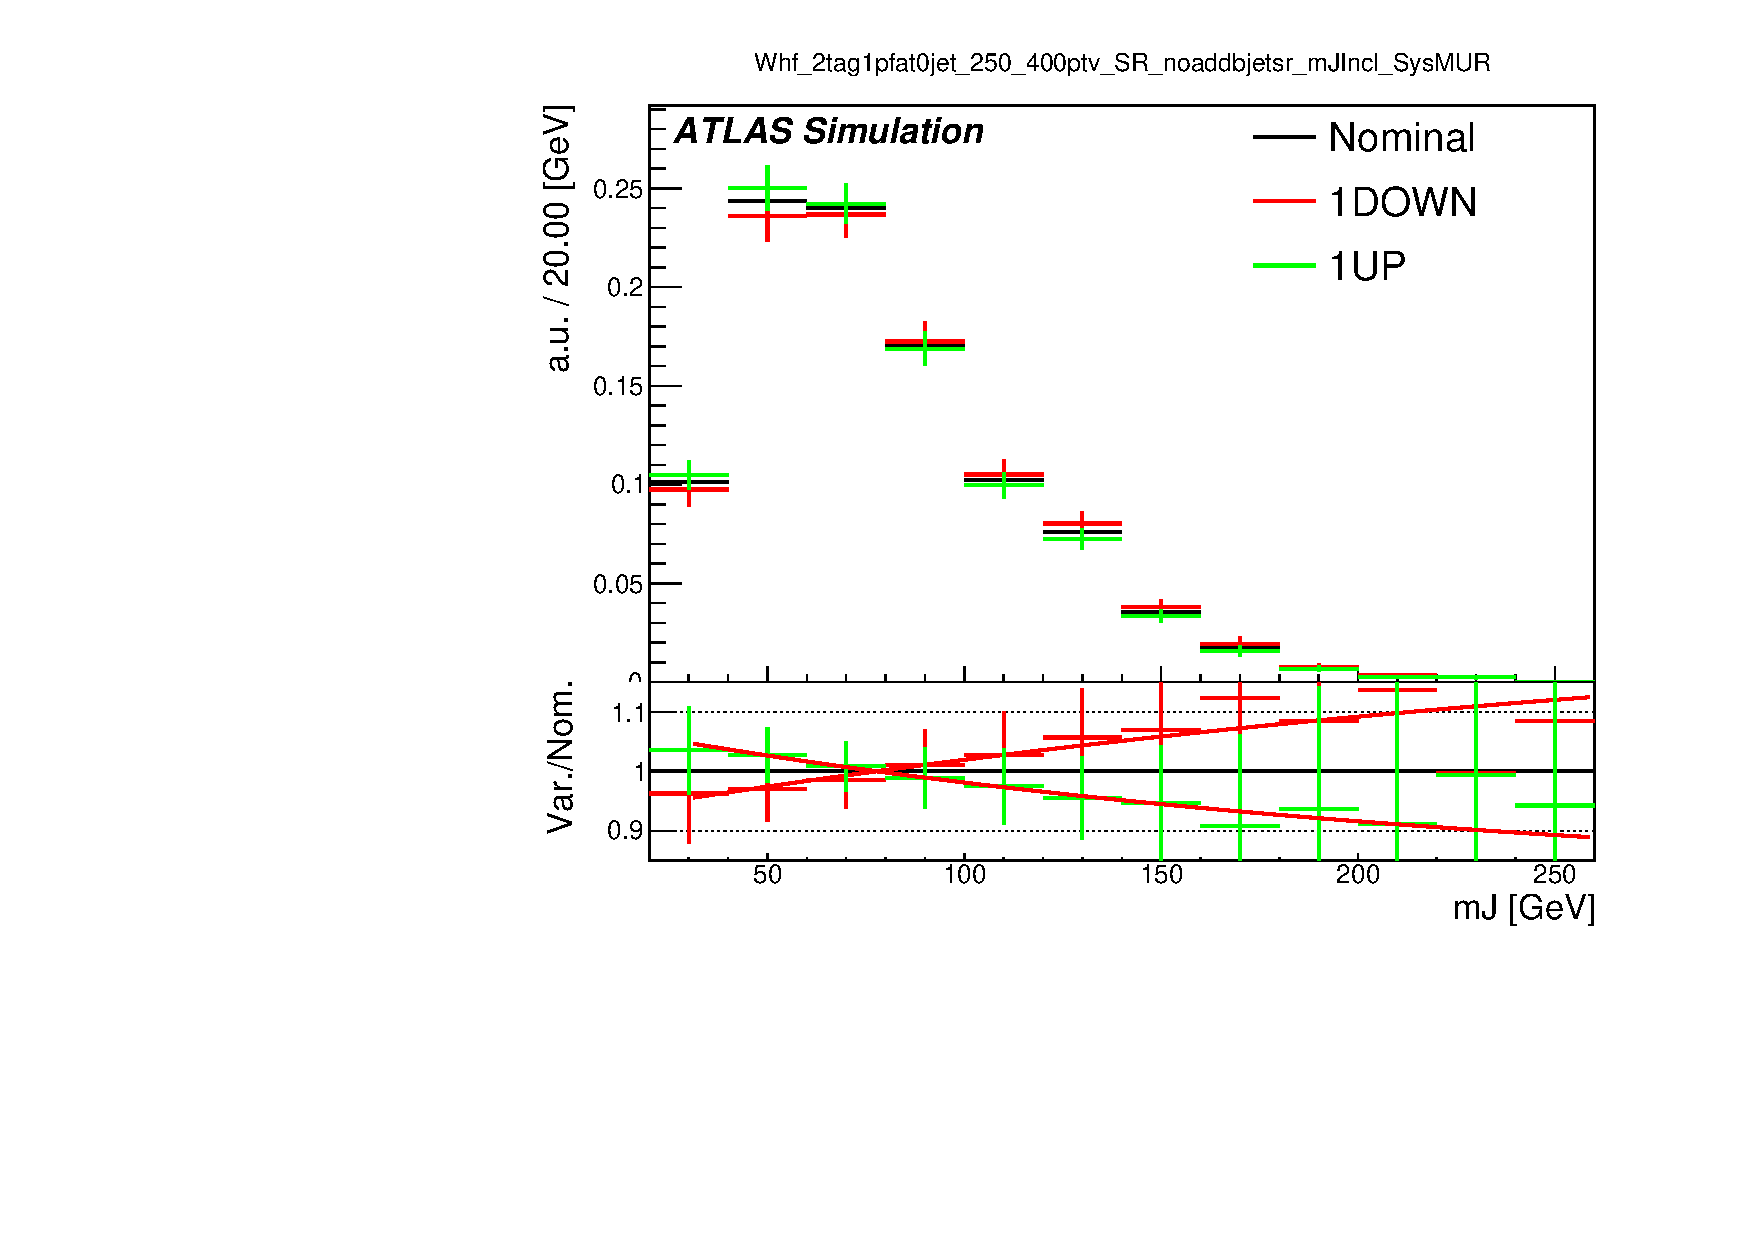
\includegraphics[width=\textwidth]{chapters/6.vhbb_boosted/figs/0L_Whf_2tag1pfat0jet_250_400ptv_SR_noaddbjetsr_mJIncl_SysMUR.pdf}
    \caption{\Whf, HP SR, medium \pTV}
    \label{fig:Vjets_SysMUR_sub1}
  \end{subfigure}%
  \hfill
  \begin{subfigure}{.5\textwidth}
    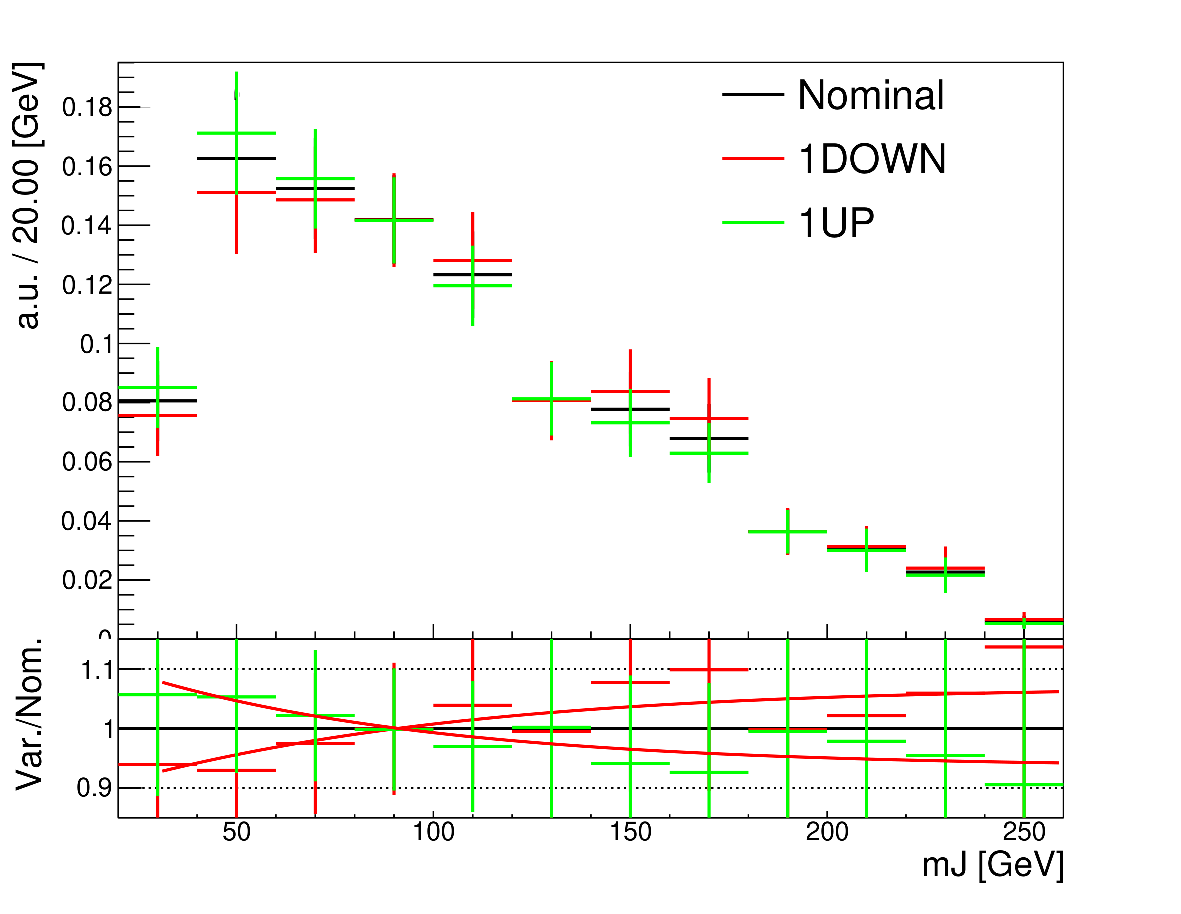
\includegraphics[width=\textwidth]{chapters/6.vhbb_boosted/figs/0L_Whf_2tag1pfat0jet_400ptv_SR_noaddbjetsr_mJIncl_SysMUR.pdf}
    \caption{\Whf, HP SR, high \pTV}
    \label{fig:Vjets_SysMUR_sub2}
  \end{subfigure}
  \begin{subfigure}{.5\textwidth}
    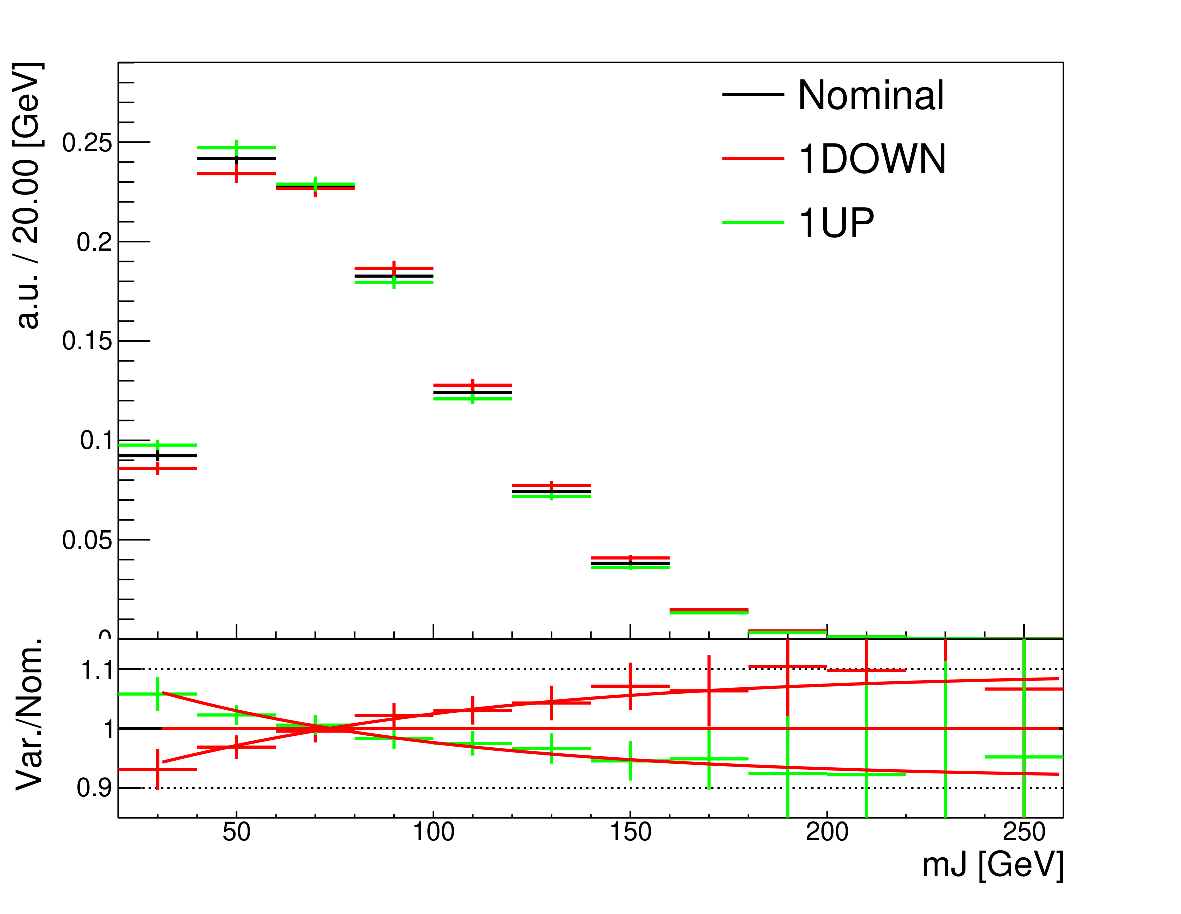
\includegraphics[width=\textwidth]{chapters/6.vhbb_boosted/figs/0L_Zhf_2tag1pfat0jet_250_400ptv_SR_noaddbjetsr_mJIncl_SysMUR.pdf}
    \caption{\Zhf, HP SR, medium \pTV}
    \label{fig:Vjets_SysMUR_sub3}
  \end{subfigure}%
  \hfill
  \begin{subfigure}{.5\textwidth}
    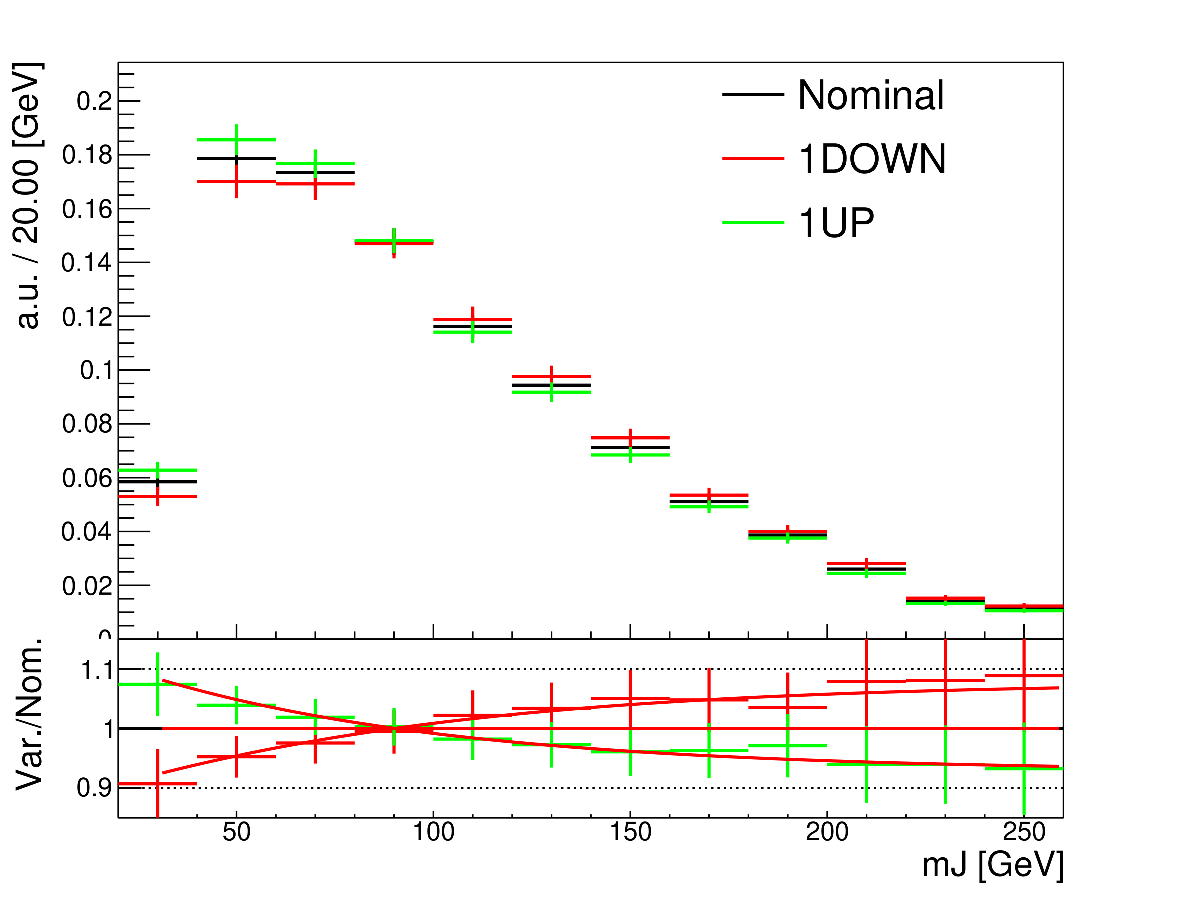
\includegraphics[width=\textwidth]{chapters/6.vhbb_boosted/figs/0L_Zhf_2tag1pfat0jet_400ptv_SR_noaddbjetsr_mJIncl_SysMUR.pdf}
    \caption{\Zhf, HP SR, medium  \pTV}
    \label{fig:Vjets_SysMUR_sub4}
  \end{subfigure}%
  \hfill
  \caption{Leading \largeR jet mass for the  \Zboson and \Whf processes in the HP SR of the \zlep channel \cite{Dao:2688371}. The renormalisation scale $\mu_r$ has been varied by a factor of 0.5 (1DOWN) and 2 (1UP). An exponential function is fitted to the ratio between the nominal and alternate samples.}
  \label{fig:Vjets_SysMUR}
\end{figure}


As an example where no significant deviation is seen, a comparison of the \mJ shapes between \SHERPA and \MADGRAPH is shown in \cref{fig:Vjets_MGSherpa_inc}.
The plots are split by process and channel, but merged in SR and \ptv bins reflecting similarities between the \mJ shapes and variations.
Due to the lack of statistically significant variation between the samples, no additional shape uncertainty was added to the fit in this case. 

\begin{figure}[!htbp]
  \centering
  \begin{subfigure}{.5\textwidth}
    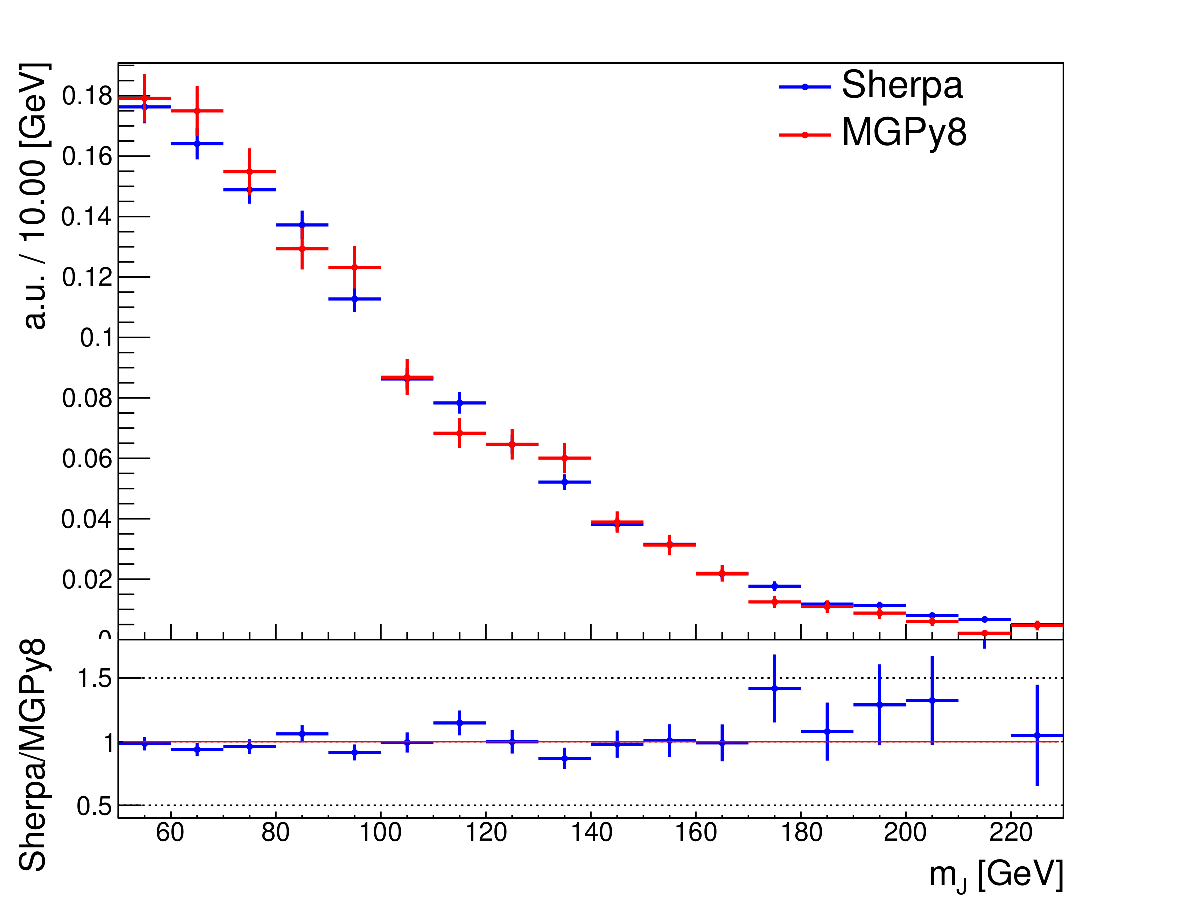
\includegraphics[width=\textwidth]{chapters/6.vhbb_boosted/figs/0L_Whf_2tag1pfat0pjet_ptvinc_SR_noaddbjetsr_mJIncl.pdf}
    \caption{\Whf, \pTV inclusive SR, \zlep channel}
    \label{fig:Vjets_MGSherpa_inc_sub1}
  \end{subfigure}%
  \hfill
  \begin{subfigure}{.5\textwidth}
    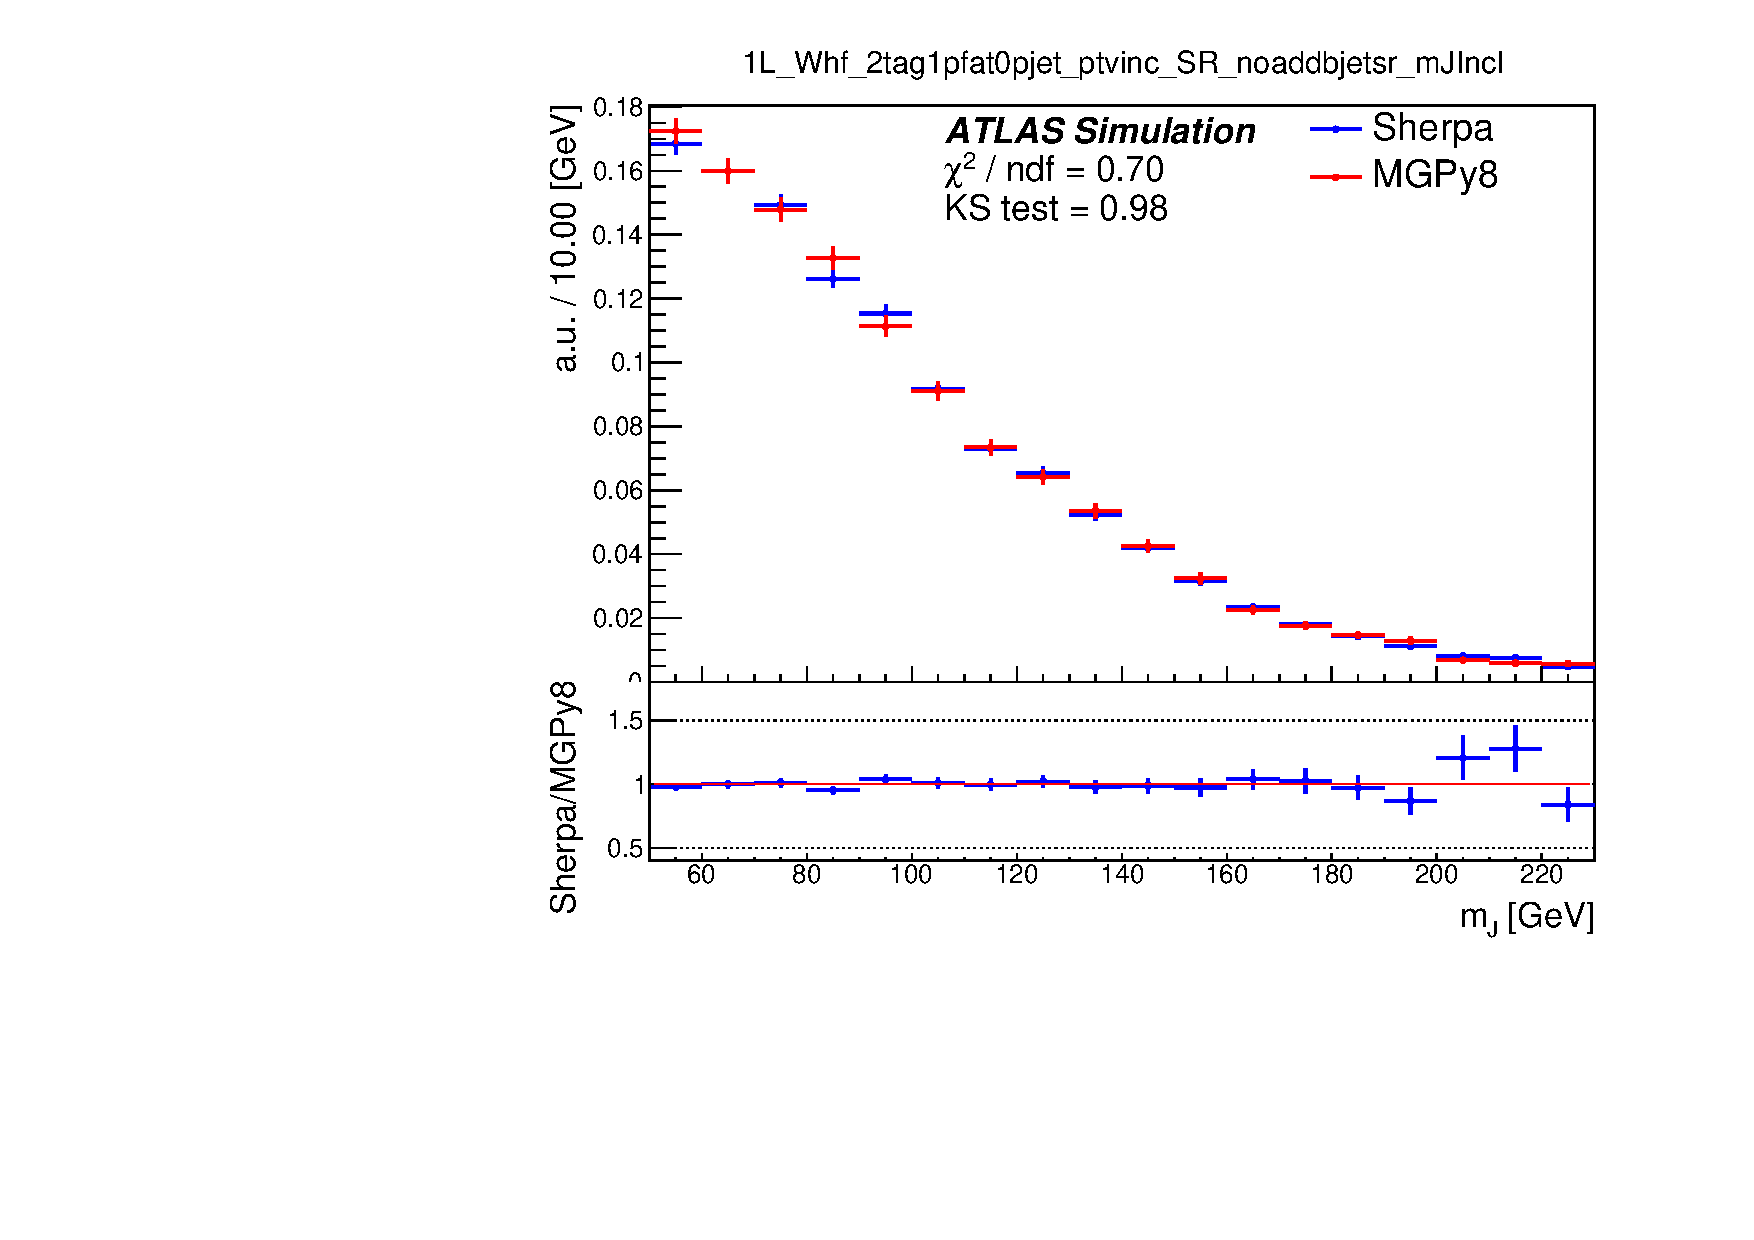
\includegraphics[width=\textwidth]{chapters/6.vhbb_boosted/figs/1L_Whf_2tag1pfat0pjet_ptvinc_SR_noaddbjetsr_mJIncl.pdf}
    \caption{\Whf, \pTV inclusive SR, \olep channel}
    \label{fig:Vjets_MGSherpa_inc_sub2}
  \end{subfigure}
  \begin{subfigure}{.5\textwidth}
    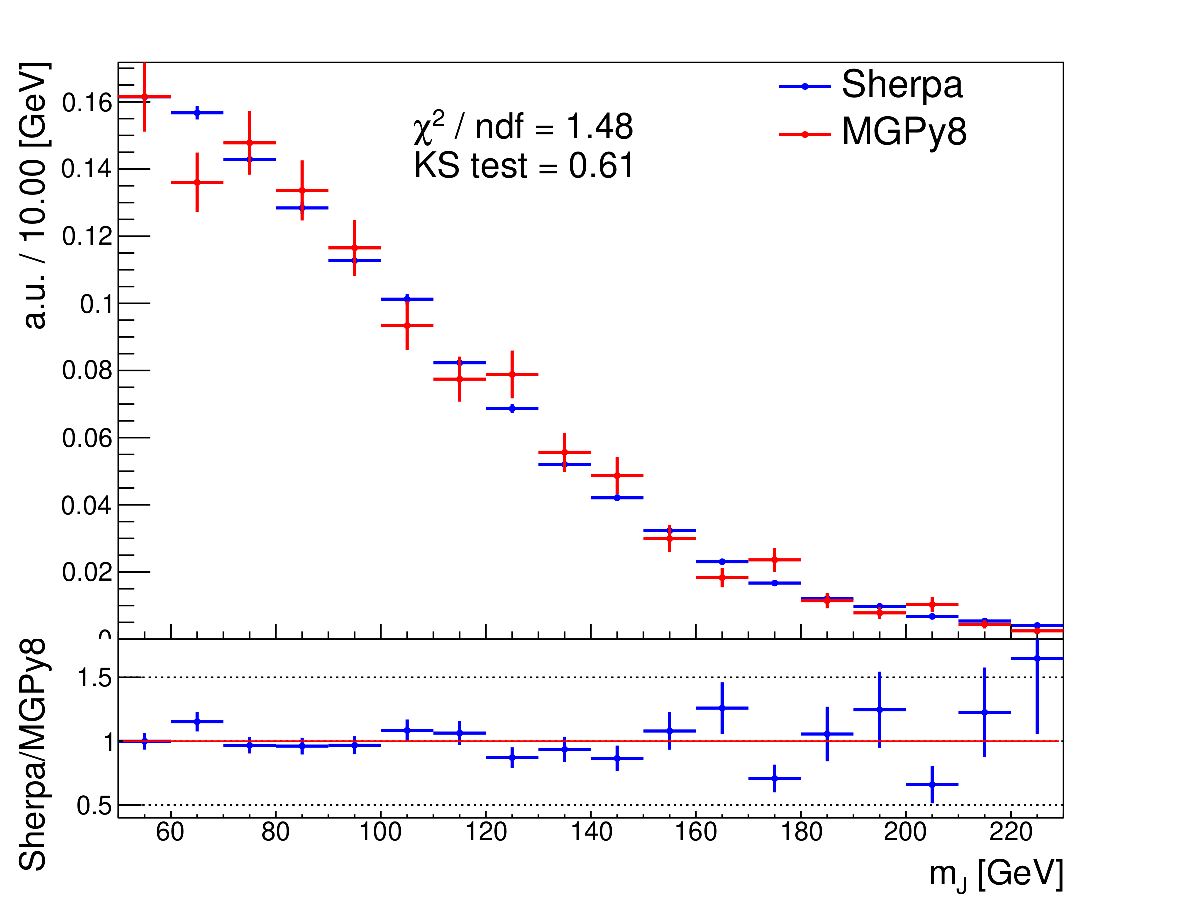
\includegraphics[width=\textwidth]{chapters/6.vhbb_boosted/figs/0L_Zhf_2tag1pfat0pjet_ptvinc_SR_noaddbjetsr_mJIncl.pdf}
    \caption{\Zhf, \pTV inclusive SR, \zlep channel}
    \label{fig:Vjets_MGSherpa_inc_sub3}
  \end{subfigure}%
  \hfill
  \begin{subfigure}{.5\textwidth}
    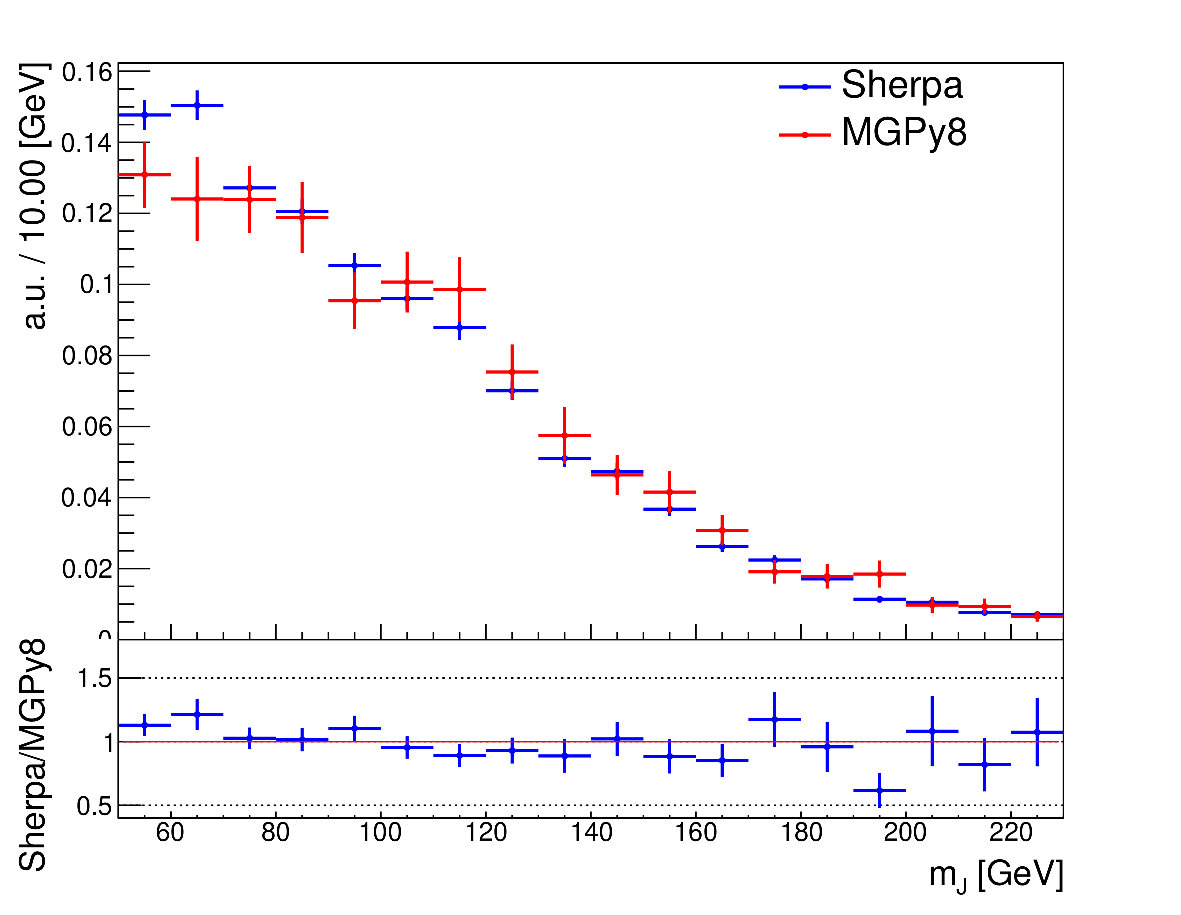
\includegraphics[width=\textwidth]{chapters/6.vhbb_boosted/figs/2L_Zhf_2tag1pfat0pjet_ptvinc_SR_mJIncl.pdf}
    \caption{\Zhf, \pTV inclusive SR, \tlep channel}
    \label{fig:Vjets_MGSherpa_inc_sub4}
  \end{subfigure}%
  \hfill
  \caption{Leading \largeR jet \mJ inclusive in \ptv for the \Vhf process modelled using both the \SHERPA+\textsc{Pythia8} (blue) and \MADGRAPH+\textsc{Pythia8} (red) samples \cite{Dao:2688371}.}
  \label{fig:Vjets_MGSherpa_inc}
\end{figure}



The impacts of variations in the factorisation scale $\mu_{F}$ and the choice of PDF set on \mJ shape were also found to be negligible in comparison with $\mu_{R}$ and are hence no additional uncertainty was added to the fit.


\subsection{Diboson Modelling}\label{sec:diboson_modelling}

The procedure to derive the uncertainties for the diboson background generally follows that of \Vjets.

The nominal diboson samples are generated using \textsc{Sherpa} 2.2.1 (except for $gg\rightarrow VV$ which uses \textsc{Sherpa} 2.2.2) with the NNPDF3.0NNLO tune.
alternate samples were generated using \textsc{Powheg} interfaced with \textsc{Pythia8}, using the AZNLO shower tune with the CTEQ6L1 PDFs \cite{Pumplin:2002:CTEQ6L1}.
Unlike \textsc{Sherpa}, \textsc{Powheg} models the off-shell $Z$ contribution at NLO.

Acceptance and shape uncertainties are derived in an analogous fashion to \Vjets as described below.

\subsubsection{Diboson Acceptance Uncertainties}

Diboson acceptance uncertainties are summarised in \cref{tab:diboson_acceptance_uncerts}.
Variations from $\mu_R$, $\mu_F$, PDF choice and an alternative generator are considered and are combined via a sum in quadrature as described in \cref{sec:vjets_modelling}.
The largest modification to the nominal acceptance is from the \textsc{Powheg+Pythia8} alternate sample.
Since the diboson contribution to the \ttbar control region is negligible, no SR-to-CR relative acceptance uncertainty is necessary.

For the $WZ$ contribution, uncertainties are derived using the 1-lepton channel and applied to all three channels.
The 1-lepton channel was used as it has the largest amount of available statistics, with the compatibility checked between the derived uncertainties and the other channels.
An additional \pct{8} channel migration uncertainty is applied on the $WZ$ 0-lepton channel.
For the $ZZ$ contribution, the normalisation uncertainty is calculated using the 2-lepton channel and applied to all three channels.
The 0- and 1-lepton channels were found to have a similar HP-to-LP relative acceptance uncertainty of \pct{18}.
The 1-lepton medium-to-high \ptv relative acceptance is estimated using the 2-lepton channel, since the 1-lepton channel had an insufficient number of events to estimate the uncertainty directly.
\pct{30} and \pct{18} channel migration uncertainties are applied in the 0- and 1-lepton channels respectively.

Since the contribution from $WW$ is negligible, dedicated studies are not performed, but a \pct{25} normalisation uncertainty is applied in all the three channels which is based on the modelling studies performed for the previous analysis \cite{HIGG-2018-04}.

\begin{table}[!htbp] 
    \footnotesize\centering
    \setlength{\tabcolsep}{0.5em} % for the horizontal padding
    \begin{tabular}{l|c|c|c|c|c|c}
    \toprule\hline
    \multicolumn{7}{c}{Diboson Acceptance Uncertainties}            
    \\ \hline
    \textbf{Bosons}     & \multicolumn{3}{c|}{{WZ}} & \multicolumn{3}{c}{{ZZ}} 
    \\ \hline
    \textbf{Channel}    &   0L      &   1L    &   2L    &   0L      &   1L      & 2L          
    \\ \hline
    Normalisation       &  \multicolumn{3}{c|}{{16\%}}    &  \multicolumn{3}{c}{{10\%}}
    \\ \hline
    HP-to-LP SR               &   \multicolumn{3}{c|}{{18\%}}   &   \multicolumn{2}{c|}{{18\%}}    &   -      
    \\ \hline
    Medium-to-high $p_T^V$    &    \multicolumn{3}{c|}{{10\%}}     &    6\%    &    \multicolumn{2}{c}{{18\%}}
    \\ \hline
    Channel Relative acceptance     &   8\%    &   \multicolumn{2}{c|}{ - }     &    30\%      &    18\%      &   -
    \\ \hline\bottomrule
    \end{tabular}
    \caption{Diboson acceptance uncertainties \cite{Dao:2688371}. All uncertainties except channel extrapolation uncertainties are fully correlated between the $ZZ$ and $WZ$ processes and channels.}
    \label{tab:diboson_acceptance_uncerts}
\end{table}
        

\subsubsection{Diboson Shape Uncertainties}

Diboson shape uncertainties are derived in a similar fashion to \Vjets.
Only the uncertainties associated with the systematic variations of $\mu_R$ and the alternate event generator have a non-negligible impact on the \mJ shape.
Variation of $\mu_R$ produces consistent \mJ shape changes across all regions and channels, and hence only a single associated uncertainty is derived, shown in \cref{fig:VV_muRFit}.
A hyperbolic tangent is fitted to the symmetrised ratio.

\begin{figure}[!htbp]
  \centering
  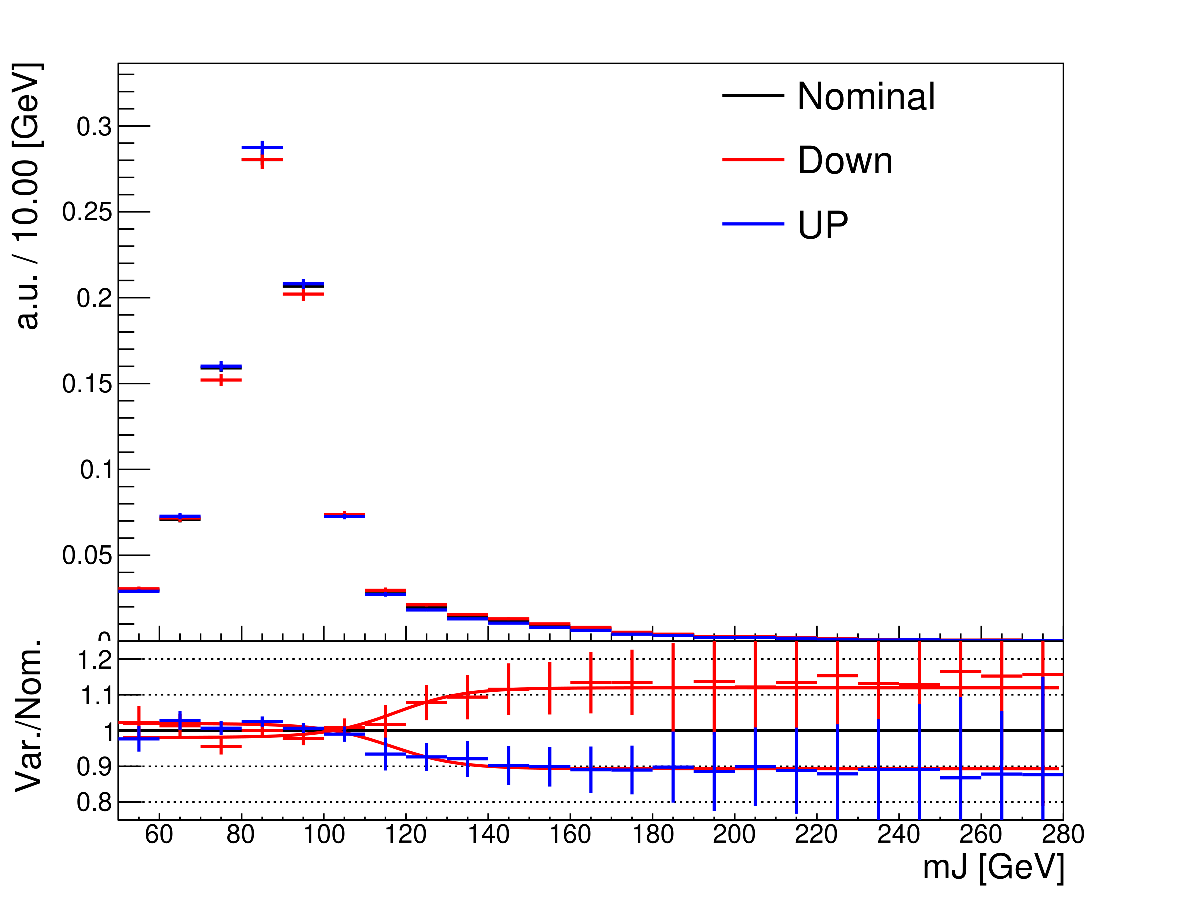
\includegraphics[width=0.5\textwidth]{chapters/6.vhbb_boosted/figs/012L_VV_2tag1pfat0pjet_ptvinc_SR_noaddbjetsr_mJIncl_SysMUR.pdf}
  \caption{
    Leading \largeR jet mass distribution for the combined $WZ$ and $ZZ$ processes, inclusive across all signal regions and lepton channels \cite{Dao:2688371}.
    The renormalisation scale $\mu_R$ has been varied by a factor of 2 (UP) and 0.5 (DOWN).
    The red and blue curves show the fitted results of the hyperbolic tangent function.
  }
  \label{fig:VV_muRFit}
\end{figure}

In the 2-lepton channel, no significant shape differences between the nominal and alternate was observed.
The comparison between the nominal \textsc{Sherpa} and alternate \POWHEG{}+\textsc{Pythia8} samples is shown in \cref{fig:VV_PP8Fit} for the 0- and 1-lepton channels for both the $WZ$ and $ZZ$ processes.
For these channels, the shape of \mJ varies in opposite directions in the LP and HP signal regions.
Shapes are similar between \ptv bins, the 0- and 1-lepton channels and for $WZ$ and $ZZ$.
In order to reduce the effects of statistical fluctuations on the fitted shape, these regions are merged before deriving the shape uncertainty.
A third order polynomial is fitted to the ratio, and this function transitions to a constant piecewise function in the high mass region to accurately represent the shape.
Dependence on the event generator was found to be negligible within statistical uncertainty in the 2-lepton channel, and so no uncertainty was applied.
All diboson shape uncertainties are fully correlated in the fit.

\begin{figure}[!htbp]
  \centering
  \begin{subfigure}{.5\textwidth}
    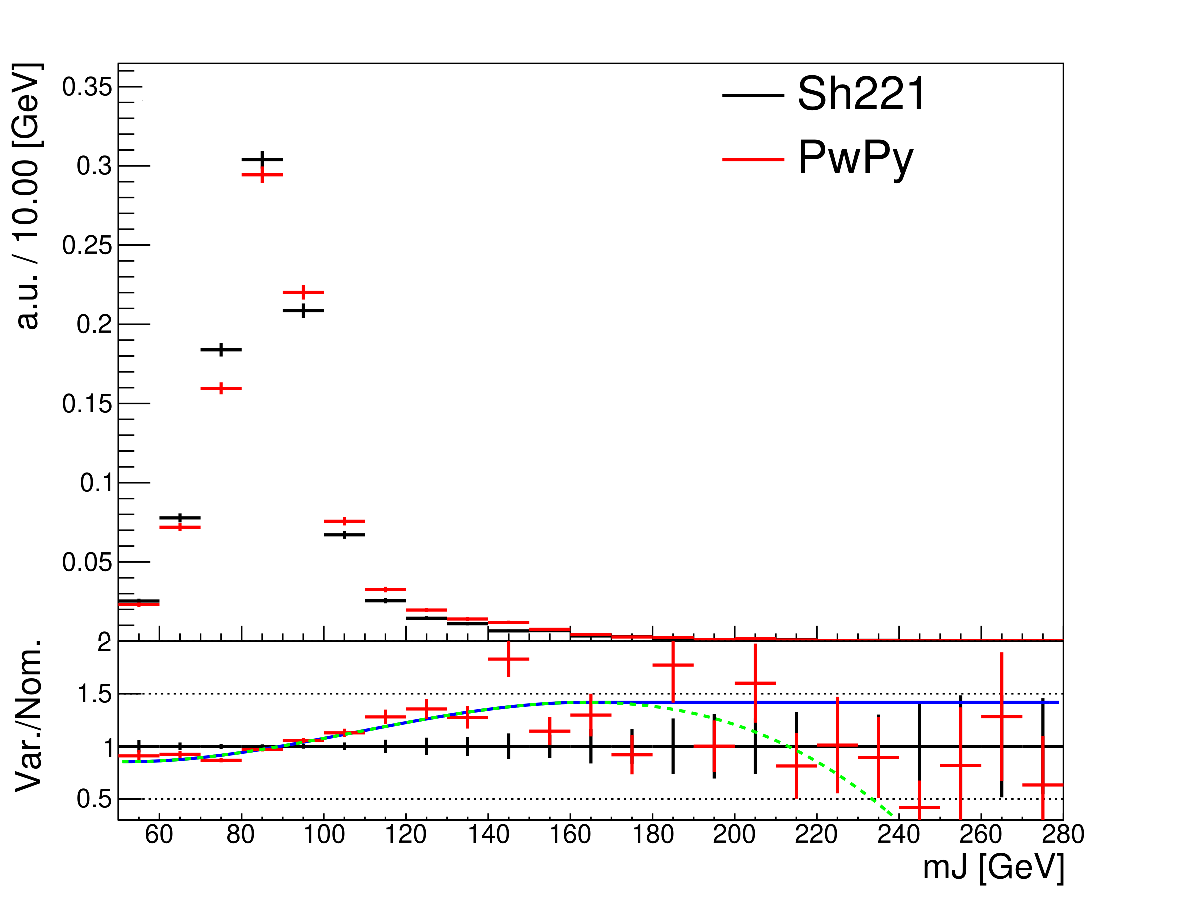
\includegraphics[width=\textwidth]{chapters/6.vhbb_boosted/figs/01L_VV_2tag1pfat0jet_ptvinc_SR_noaddbjetsr_mJIncl_SysPwPy.pdf}
    \caption{High purity signal region}
    \label{fig:VV_PP8Fit_sub1}
  \end{subfigure}%
  \begin{subfigure}{.5\textwidth}
    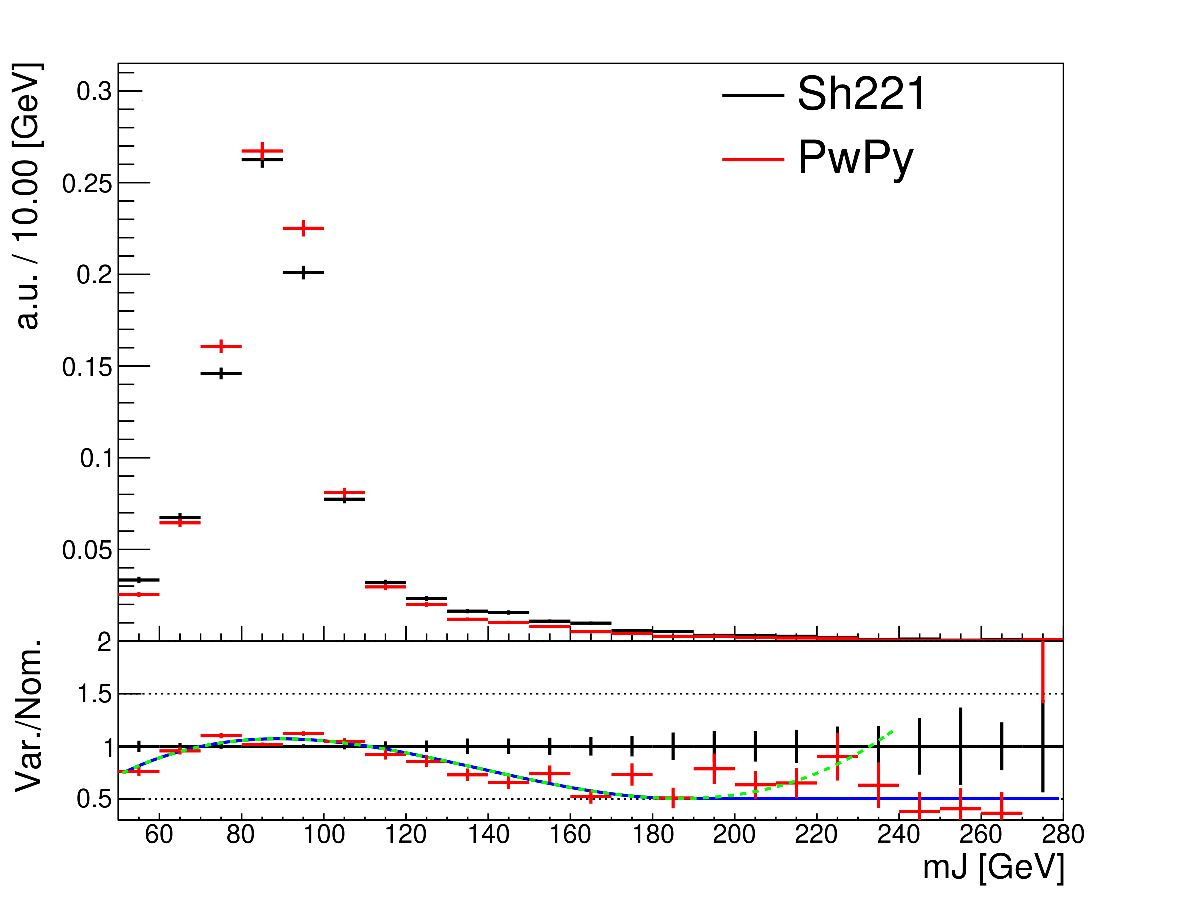
\includegraphics[width=\textwidth]{chapters/6.vhbb_boosted/figs/01L_VV_2tag1pfat1pjet_ptvinc_SR_noaddbjetsr_mJIncl_SysPwPy.pdf}
    \caption{Low purity signal region}
    \label{fig:VV_PP8Fit_sub2}
  \end{subfigure}
  \caption{
    Comparison of the shapes of the \largeR jet mass \mJ between \SHERPA (Sh221) (black) and \POWHEG{}+\textsc{Pythia8} (PwPy) (red) samples from the $WZ$ and $ZZ$ processes in high and low purity signal regions, integrated over \pTV regions and the 0- and 1-lepton channels \cite{Dao:2688371}.
    The dashed green line shows the fitted third order polynomial function and the blue lines show the function after protection is added in the high mass region.
  }
  \label{fig:VV_PP8Fit}
\end{figure}


\subsection{\texorpdfstring{\ttbar}{ttbar} and single-top Modelling}

The main features of the systematic uncertainties on the remaining two modelled backgrounds, \ttbar and single-top, are described below.

The modelling of the \ttbar background uses a \POWHEG{}+\textsc{Pythia8} nominal sample.
Two alternate samples were considered: \POWHEG{}+\textsc{Herwig7} (providing an alternate parton shower model) and \textsc{MadGraph5+Pythia8.2} (providing an alternate hard scatter model).
Effects of initial and final state radiation (ISR and FSR, respectively) were assessed using internal weight variations in the nominal sample.
Acceptance and shape uncertainties were derived for each of the variations.
The largest contribution for the acceptance uncertainties is due to the matrix element calculation, with the parton showering model being second.
The ISR and FSR acceptance uncertainties were found to be subdominant.
Acceptance uncertainties for the single-top background are enumerated in \cref{tab:ttbar_acceptance_uncerts}.
For the shape uncertainties, only the ISR and parton showering variations have non-negligible impacts on the \mJ shape.

\begin{table}[!htbp] 
    \footnotesize\centering
    \setlength{\tabcolsep}{0.5em} % for the horizontal padding
    \begin{tabular}{l|c}
    \toprule\hline
    \multicolumn{2}{c}{\ttbar Acceptance Uncertainties}            
    \\ \hline
    HP-to-LP SR       &  \pct{18}
    \\ \hline
    Medium-to-high $p_T^V$       &  \pct{20}
    \\ \hline
    SR-to-CR       &  \pct{6}
    \\ \hline\bottomrule
    \end{tabular}
    \caption{
        Acceptance uncertainties for the \ttbar background.
        The uncertainties on the 0- and 1-lepton channels are found to be similar, but are conservatively taken to be uncorrelated. 
        The HP-to-LP SR uncertainty is applied in the HP SR.
        The Medium-to-high $p_T^V$ uncertainty is applied in the high $p_T^V$ bin, and is larger than the computed uncertainty in order to account for the known mismodelling of the \ttbar \pt spectrum.
        \cite{Dao:2688371}.
    }
    \label{tab:ttbar_acceptance_uncerts}
\end{table}
        

The dominant process contributing to the single-top background is $\Wboson t$ production for the 0- and 1-lepton channels.
The same nominal and alternate generators are used as for the \ttbar background.
Again, ISR and FSR variations are obtained from internal weight variations in the nominal sample.
At higher orders in QCD, diagrams contributing to the $\Wboson t$ production process can also be found in leading-order \ttbar
production processes.
To account for the arising interference effects, the diagram removal (DR) scheme in \rcite{Frixione:2008yi} was employed for the nominal sample.
The uncertainty on the DR scheme was assessed using an alternate sample using a diagram subtraction (DS) method which removes interference at the generator level.
The largest sources of acceptance and shape uncertainties were due to this DS-DR variation.
Acceptance uncertainties for the single-top background are enumerated in \cref{tab:stop_acceptance_uncerts}.

\begin{table}[!htbp] 
    \footnotesize\centering
    \setlength{\tabcolsep}{0.5em} % for the horizontal padding
    \begin{tabular}{l|c}
    \toprule\hline
    \multicolumn{2}{c}{Single-Top Acceptance Uncertainties}            
    \\ \hline
    Normalisation       &  \pct{20}
    \\ \hline
    HP-to-LP SR       &  \pct{25}
    \\ \hline
    Medium-to-high $p_T^V$       &  \pct{20}
    \\ \hline
    SR-to-CR       &  \pct{30}
    \\ \hline
    Channel Relative acceptance       &  \pct{20}
    \\ \hline\bottomrule
    \end{tabular}
    \caption{
        Single-top acceptance uncertainties. 
        Uncertainties are derived in the 1-lepton channel but applied in a correlated fashion to both the 0- and 1-lepton channels.
        The HP-to-LP SR uncertainty is applied in the HP SR.
        The Medium-to-high $p_T^V$ uncertainty is applied in the high $p_T^V$ bin.
        The channel relative acceptance uncertainty is applied in the 0-lepton channel.
        \cite{Dao:2688371}.
    }
    \label{tab:stop_acceptance_uncerts}
\end{table}
        

\subsection{Signal Modelling}

The modelling of the systematic uncertainties affecting the signal processes follows the procedure described in Refs.~\cite{HIGG-2018-50,deFlorian:2016spz,HIGG-2016-29}.
The $qq \rightarrow VH$ signal samples are generated with \POWHEGBOX[v2]+\textsc{GoSam} at next-to-leading order (NLO) accuracy in QCD. 
An additional $gg \rightarrow ZH$ sample is generated using \POWHEGBOX[v2] at leading order (LO) in QCD.
In both cases, the generated events are interfaced with \PYTHIAV{8} for the parton showering modelling.
An alternate \textsc{Herwig7} sample is used to assess the uncertainty on the parton showering model.
Recommended systematic uncertainties on the signal production cross-sections and \Hbb branching ratio from the LHC Higgs Cross Section Working Group are applied~\cite{Dittmaier:2012vm,Heinemeyer:2013tqa}.
This includes acceptance and shape uncertainties arising from missing higher-order QCD and electroweak corrections, PDF uncertainties, renormalisation and factorisation scales, and an alternate parton showering model.

\section{Statistical Treatment}\label{sec:vhbb_fit}

%Selected events are used to perform a statistical test of the background-only hypothesis, i.e. a model which does not include the \VHbb process.
%The test involves 
A binned global maximum-profile-likelihood fit of the \mJ distribution is performed to extract information on the signal, combining all the analysis regions defined in \cref{tab:SR_CR_definition}.
%The test is based on the profile likelihood ratio test statistic.
The signal strength $\mu = \sigma / \sigma_{\textnormal{SM}}$ is defined as the ratio between the observed and predicted cross-sections, where $\mu = 0$ corresponds to the background-only hypothesis and $\mu = 1$ corresponds to the SM prediction.
This is a parameter of interest (POI) which acts to scale the total number of signal events, and is determined during the fit procedure.

The present analysis makes use of two POIs.
The first, \muVH, is the signal strength for the \VHbb process, the primary process under investigation.
The diboson production strength \muVZ for the \VZbb process is measured simultaneously and provides a validation of the analysis apparatus used for the primary \Hbb measurement.
Alongside the two POIs, the predictive model depends on several parameters which are not the primary target of measurement, and represent the systematic uncertainties discussed previously.
These parameters are called nuisance parameters (NPs), collectively referred to as $\theta$.
Freely floating background normalisations are implemented as NPs and are also extracted during the fitting processes.


\subsection{Likelihood Function}

The statistical setup treats each bin as a Poisson counting experiment and is based on the \textsc{RooStats} framework \cite{moneta2010roostats}.
The combined likelihood over $N$ bins is constructed as the product of Poisson probabilities in each bin.
Considering the simplified case of a single signal strength parameter $\mu$, and neglecting sources of systematic or statistical uncertainty, this is given by
%
\begin{equation}
    \mathcal{L}(\mu) = \prod_{i=1}^N \frac{(\mu s_i + b_i)^{n_i}}{n_i!} \exp \left[ - (\mu s_i + b_i) \right],
\end{equation}
%
where $s_i$ ($b_i$) is the expected number of signal (background) events in bin $i$, and $n_i$ is the number of observed data events in bin $i$.

\subsubsection{Treatment of Uncertainties}

Systematic uncertainties can modify the predicted signal and background yields $s_i$ and $b_i$. 
Each source of systematic uncertainty is taken into account by adding an additional NP $\theta_j$ to the likelihood in the form of a Gaussian cost function.
The combined effect of the NPs is then
%
\begin{equation}
  \mathcal{L}(\theta) = 
  \prod_{j = 1}^{N_\theta}
  \frac{1}{\sqrt{2 \pi \sigma_j}}
  \exp\left[ \frac{- (\theta_j - \hat{\theta}_j)^2}{2 \sigma_j^2} \right] ,
\end{equation}
%
where $N_\theta$ is the number of NPs, $\theta_j$ is the nominal value of the $j$th NP, $\hat{\theta}_j$ is the fitted value, and $\sigma_j$ is the corresponding associated prior uncertainty on the NP.
As the fitted value $\hat{\theta}_j$ deviates from it's nominal value, a cost is introduced.
The presence of NPs modifies the likelihood as 
%
\begin{equation}
    \mathcal{L}(\mu) \rightarrow \mathcal{L}(\mu, \theta) = \mathcal{L}(\mu) \mathcal{L}(\theta) .
\end{equation}
%
The predicted signal and background yields are also modified by the presence of the NPs with
%
\begin{equation}
  s_i \rightarrow s_i(\theta) , \quad b_i \rightarrow b_i(\theta) .
\end{equation}
%
For NPs which are left freely floating in the fit, no corresponding Gaussian constraints are added to the likelihood.

The pull of a NP is defined as the difference between the fitted value $\hat{\theta}_j$ and the nominal value $\theta_j$, divided by the uncertainty on the NP $\sigma_j$.
To obtain the  uncertainty on the pull of a NP, the following procedure is used.
The Hessian matrix $\mathbf{H}$ is calculated as


\begin{equation}
  \mathbf{H} =
  \begin{bmatrix}
    \dfrac{\partial^{2}\mathcal{L}}{\partial \theta_{1}^{2}} &
    \dfrac {\partial^{2}\mathcal{L}}{\partial \theta_{1} \partial \theta_{2}}& \cdots &
    \dfrac{\partial ^{2}\mathcal{L}}{\partial \theta_{1} \partial \theta_{n}}\\[2ex]
    %
    \dfrac{\partial^{2}\mathcal{L}}{\partial \theta_{2} \partial \theta_{1}}&
    \dfrac{\partial^{2}\mathcal{L}}{\partial \theta_{2}^{2}}&\cdots &
    \dfrac{\partial^{2}\mathcal{L}}{\partial \theta_{2} \partial \theta_{n}}\\[2ex]
    %
    \vdots &\vdots &\ddots &\vdots \\[2.2ex]
    \dfrac{\partial^{2}\mathcal{L}}{\partial \theta_{n} \partial \theta_{1}}&
    \dfrac{\partial ^{2}\mathcal{L}}{\partial \theta_{n} \partial \theta_{2}}&\cdots &
    \dfrac{\partial^{2}\mathcal{L}}{\partial \theta_{n}^{2}}
  \end{bmatrix}   . 
\end{equation}

Taking the inverse of the Hessian matrix $\mathbf{H}^{-1}$ yields the covariance matrix, from which the post-fit uncertainties on the different NPs can be extracted.
If the post-fit uncertainty is smaller than the nominal uncertainty, additional information about the NP has been extracted by the fit, and NP is said to be \textit{constrained}.

Following \rcite{Barlow:249779}, the statistical uncertainty on the simulated events is implemented using a dedicated NP for each bin which can scale the background yield in that bin.
Statistical NPs are also implemented using a Gaussian constraint.

\subsubsection{Smoothing and Pruning}

To simplify the fit to reduce and improve its robustness, systematic uncertainties are smoothed and pruned.
Smoothing accounts for the large statistical uncertainty present in some samples that can lead to unphysical fluctuations in the shape systematics.
The smoothing procedure relies on the assumption that the impact of systematics should be approximately monotonic and correlated between neighbouring bins.

In addition to smoothing, pruning is the process of removing from the fit those systematics which only have a very small effect.
This improves the stability of the fit by reducing the number of degrees of freedom.
Acceptance uncertainties are pruned in a given region if they have a variation of less than \pct{0.5}, or if the up and down variations have the same sign in that region.
Shape uncertainties are pruned in a given region if the deviation in each bin is less than \pct{0.5} in that region.
In addition, acceptance and shape uncertainties are neglected in a given region for any background which makes up less than \pct{2} of the total background in that region.


\subsubsection{Fit Procedure and Statistical Tests}

The best-fit value of $\mu$, denoted $\hat\mu$, is obtained via an unconditional maximisation of the likelihood.
The likelihood is also used to construct a statistical test which can confirm or reject the background-only hypothesis.
The test statistic $q_\mu$ is constructed from the profile likelihood ratio,
%
\begin{equation}
  q_\mu = -2 \ln \frac{\mathcal{L(\mu, \hat{\hat{\theta}}_\mu )} } { \mathcal{L(\hat{\mu}, \hat{\theta}}) }
\end{equation}
%
where $\hat{\mu}$ and $\hat{\theta}$ are chosen to maximise the likelihood $\mathcal{L}$, and the profile value $\hat{\hat{\theta}}_\mu$ is obtained from a conditional maximisation of the likelihood for a specific choice of $\mu = 0$ corresponding to the background-only hypothesis.
% i.e. this is the profile likelihood (double hat term)

The test statistic is used to construct a $p$-value which is used to probe the background-only hypothesis.
The $p$-value is typically reported in terms of the significance $Z$, defined as the number of standard deviations for a Gaussian Normal distribution which will produce a one-sided tail integral equal to the $p$-value, as in
%
\begin{equation}
  p = \int_Z^{\infty} \frac{1}{\sqrt{2 \pi}} e^{-x^2/2} ~\mathrm{d} x
  = 1 - \Phi(Z) .
\end{equation}
%
Typically a value of $Z=3$ constitutes \textit{evidence} of a processes, while $Z=5$ is required for a \textit{discovery}, or \textit{observation}.
Alongside the $p$-value, the best-fit value of the signal strength $\hat\mu$ and its corresponding uncertainty are quoted, and compared to their expected values.
More detail on the statistical methodology can be found in \rcite{Cowan:2010js}.

\begin{comment}
  All initial background distribution shapes prior to the fit (described in Section 8), except those for multijet, are estimated from the samples of simulated events. The multijet shape and normalisation are determined using data  
  The normalisation on the diboson background is left floating in the fit, i.e. measured simultaneously along with the $VH$ signal
\end{comment}


\subsection{Background Normalisations}

The backgrounds which can be constrained by the fit are left freely floating and the corresponding normalisation factors are
extracted. 
Normalisation factors (NF), represent the value by which the predicted normalisations are scaled, and are implemented for the dominant backgrounds
(\ttbar, \Zhf, \Whf).
The NFs are also subdivided into different regions of phase-space for \ttbar, given it is possible to obtain a strong constraint in the individual channels.
This also removes the need for an extrapolation uncertainty.

%A single normalisation factor is used for \Whf and \Zhf, which constitue more than \pct{90} of the total \Vjets background, since the use of independent factors in different channels were found to be compatible.


The normalisations and shapes of all other backgrounds, with the exception of the multijet background which is estimated using a data driven technique, are initialised using the nominal samples and the state-of-the art process normalisations, as outlined in \cref{tab:vhbb_samples}.
%Note: some of the normalisations come from the generator predictions and some from state-of-the-art calculations, this is all detailed in Table 7.2, but be aware of this.


\subsection{Asimov Dataset \& Expected Results}\label{sec:fit_expected}

The Asimov dataset is constructed by replacing the data with the sum of the signal and background predictions $n_i = s_i + b_i$.
A fit to this dataset using the nominal values of the NPs from the simulation will recover the input values and is useful for studying the expected result, in addition to constraints on and correlations between the NPs.

Alternatively, a conditional fit to the Asimov dataset can be performed using values of the background NPs which are determined from an unconditional fit to data.
The signal NPs and POIs are fixed at their nominal values from the SM simulation.
The result of this fit can be used to calculate expected (median) significances given a more realistic background model, which can be compared to their observed values, as is done in \cref{sec:signal_strengh_sigs}.
%The fit is conditional on the signal strength parameter, which is fixed at its nominal value.

\section{Results}\label{sec:vhbb_results}

In the present analysis, the two signal strength parameters \muVH and \muVZ are extracted from a simultaneous maximisation of the likelihood described in \cref{sec:vhbb_fit}.
The results of the analysis are summarised in this section.
Post-fit \mJ distributions are shown in \cref{sec:postfit_plots}.
The observed signal strengths are given in \cref{sec:signal_strengh_sigs}, along with observed and expected significances.
Finally in \cref{sec:sys_results} the impact of systematic uncertainties on the results is examined.



\subsection{Post-fit Results}\label{sec:postfit_plots}

In addition to the observed significance and signal strength, it is also necessary to study the post-fit \mJ yields and  distributions to compare the level of the agreement between the simulation (using the best-fit values of the signal strength $\hat{\mu}$ and the NP $\hat{\theta}$) and the data.
The best-fit values $\hat{\mu}$ and $\hat{\theta}$ are obtained from an unconditional fit to data over all analysis regions.
The post-fit background normalisation factors extracted from the unconditional fit to data fit are shown in \cref{tab:bkg_norms}, and the post-fit yields are presented in \cref{tab:postfityield0L}, \cref{tab:postfityield1L}, and \cref{tab:postfityield2L} for the 0-, 1- and 2-lepton channels, respectively.

\begin{table}[hptb]
    \footnotesize\centering
    \setlength{\tabcolsep}{0.5em} % for the horizontal padding
    \begin{tabular}{lc}
        \toprule\hline
        Process & Normalisation factor \\
        \hline
        \ttbar 0-lepton & $0.88 \pm 0.10$ \\ 
        \ttbar 1-lepton & $0.83 \pm 0.09$ \\ 
        \Whf\  &  $1.12 \pm 0.14$ \\
        \Zhf\ &  $1.32 \pm 0.16$ \\
        \hline\bottomrule
    \end{tabular}
    \caption{
        Factors applied to the nominal normalisations of the \ttbar, \Whf, and \Zhf backgrounds, as obtained from the likelihood fit \cite{HIGG-2018-52}.
        The errors represent the combined statistical and systematic uncertainties.
    }
    \label{tab:bkg_norms}
\end{table}

% note this line causes the following warning:
% Overfull \hbox (5.55814pt too wide) in paragraph at lines 38--62
\begin{table}[!htpb]
    \small
    \scriptsize\centering
    %\setlength{\tabcolsep}{0.5em} % for the horizontal padding
    %\setlength{\extrarowheight}{2pt}
    \begin{tabular}{ l | r @{$\pm$} l | r @{$\pm$} l | r @{$\pm$} l | r @{$\pm$} l | r @{$\pm$} l | r @{$\pm$} l }
    \toprule\hline
    & \multicolumn{6}{c|}{250 GeV $< \pTV \leq$ 400 GeV}  & \multicolumn{6}{c}{$\pTV >$ 400 GeV} \\ 
    \cline{2-13}
    Processes & \multicolumn{2}{c|}{HP}    & \multicolumn{2}{c|}{LP}    & \multicolumn{2}{c|}{CR}    & \multicolumn{2}{c|}{HP}    & \multicolumn{2}{c|}{LP}    & \multicolumn{2}{c}{CR}    \\ \hline
    Signal  & 21.93 & 11.17 & 18.99 & 9.76 & 1.05 & 0.54 & 5.69 & 2.88 & 5.85 & 3.01 & 0.33 & 0.17\\
    W+t  & 14.70 & 5.37 & 45.55 & 19.44 & 17.18 & 8.09 & 2.03 & 0.98 & 8.93 & 6.33 & 3.76 & 2.49\\
    other t+X  & 0.79 & 0.03 & 3.18 & 0.66 & 4.51 & 1.28 & \multicolumn{2}{c|}{-} & 0.66 & 0.03 & 0.11 & 0.00\\
    \ttbar   & 75.19 & 13.60 & 423.85 & 36.12 & 539.21 & 31.39 & 7.54 & 1.77 & 38.20 & 6.75 & 44.07 & 7.43\\
    VZ  & 77.01 & 17.09 & 87.70 & 19.36 & 6.16 & 1.56 & 17.30 & 4.10 & 28.77 & 6.55 & 2.79 & 0.72\\
    WW  & \multicolumn{2}{c|}{-} & 2.15 & 0.05 & 0.24 & 0.01 & 0.33 & 0.02 & 1.80 & 0.06 & \multicolumn{2}{c}{-}\\
    Whf  & 100.78 & 20.01 & 331.31 & 59.54 & 29.97 & 21.85 & 20.19 & 6.24 & 59.82 & 17.91 & 6.61 & 5.09\\
    Wcl  & 5.13 & 2.31 & 8.44 & 3.24 & 0.46 & 0.01 & 0.99 & 0.69 & 2.77 & 1.14 & 0.19 & 0.07\\
    Wl  & 5.61 & 3.93 & 4.61 & 2.45 & 0.16 & 0.00 & 1.41 & 2.06 & 2.67 & 1.67 & 0.57 & 0.36\\
    Zhf  & 318.76 & 35.27 & 548.71 & 61.84 & 76.97 & 21.47 & 86.79 & 10.63 & 184.99 & 21.43 & 25.76 & 7.43\\
    Zcl  & 3.97 & 1.63 & 6.74 & 2.68 & 0.83 & 0.02 & \multicolumn{2}{c|}{-} & 6.36 & 2.73 & 0.93 & 0.41\\
    Zl  & 1.34 & 0.67 & 3.61 & 2.14 & 0.42 & 0.01 & 1.05 & 0.63 & 3.68 & 2.47 & 0.29 & 0.16\\
    \hline
    Data  & \multicolumn{2}{c|}{623} & \multicolumn{2}{c|}{1493} & \multicolumn{2}{c|}{683} & \multicolumn{2}{c|}{146} & \multicolumn{2}{c|}{330} & \multicolumn{2}{c}{85}\\
    Background  & 603 & 25 & 1466 & 36 & 676 & 25 & 138 & 9 & 339 & 15 & 85 & 7\\
    \hline\bottomrule
    \end{tabular}
    \caption{Post-fit yields in the \zlep channel. Combined statistical and systematic uncertainties are shown \cite{Dao:2688371}. }
    \label{tab:postfityield0L}
\end{table}


\begin{table}[!htpb]
    \small
    \scriptsize\centering
    %\setlength{\tabcolsep}{0.5em} % for the horizontal padding
    %\setlength{\extrarowheight}{2pt}
    \begin{tabular}{ l | r @{$\pm$} l | r @{$\pm$} l | r @{$\pm$} l | r @{$\pm$} l | r @{$\pm$} l | r @{$\pm$} l }
    \toprule\hline
    & \multicolumn{6}{c|}{250 GeV $< \pTV \leq$ 400 GeV}  & \multicolumn{6}{c}{$\pTV >$ 400 GeV} \\ 
    \cline{2-13}
    Processes & \multicolumn{2}{c|}{HP}    & \multicolumn{2}{c|}{LP}    & \multicolumn{2}{c|}{CR}    & \multicolumn{2}{c|}{HP}    & \multicolumn{2}{c|}{LP}    & \multicolumn{2}{c}{CR}    \\ \hline
    Signal  & 24.23 & 12.34 & 18.02 & 9.29 & 0.88 & 0.45 & 7.84 & 3.96 & 7.50 & 3.87 & 0.39 & 0.20\\
    W+t  & 64.35 & 21.12 & 159.95 & 75.14 & 73.44 & 29.96 & 16.40 & 7.31 & 53.28 & 41.74 & 21.16 & 15.36\\
    other t+X  & 1.92 & 0.48 & 16.33 & 0.31 & 21.89 & 6.18 & 0.13 & 0.01 & 1.70 & 0.06 & 3.95 & 1.40\\
    \ttbar   & 234.76 & 30.21 & 1189.51 & 75.91 & 1758.08 & 57.99 & 50.87 & 7.34 & 226.85 & 23.98 & 340.61 & 25.32\\
    VZ  & 35.94 & 8.87 & 56.30 & 13.98 & 4.93 & 1.38 & 8.63 & 2.30 & 20.02 & 5.29 & 2.61 & 0.84\\
    WW  & \multicolumn{2}{c|}{-} & 6.48 & 1.63 & \multicolumn{2}{c|}{-} & \multicolumn{2}{c|}{-} & 4.35 & 1.32 & 0.93 & 0.03\\
    Whf  & 265.13 & 27.68 & 617.81 & 63.56 & 59.91 & 21.90 & 91.42 & 11.51 & 238.81 & 29.53 & 26.55 & 9.84\\
    Wcl  & 7.33 & 2.95 & 13.81 & 5.65 & 2.10 & 0.04 & 6.23 & 2.49 & 10.17 & 4.09 & 0.63 & 0.02\\
    Wl  & 2.99 & 1.47 & 5.66 & 3.39 & 0.65 & 0.01 & 2.21 & 1.35 & 7.67 & 4.98 & 0.31 & 0.01\\
    Zhf  & 10.16 & 1.24 & 24.61 & 2.46 & 3.45 & 0.41 & 2.12 & 0.30 & 6.56 & 0.79 & 0.98 & 0.12\\
    Zcl  & 0.02 & 0.00 & 0.75 & 0.02 & \multicolumn{2}{c|}{-} & \multicolumn{2}{c|}{-} & 0.33 & 0.01 & 0.02 & 0.00\\
    Zl  & \multicolumn{2}{c|}{-} & 0.49 & 0.01 & 0.03 & 0.00 & 0.30 & 0.19 & 0.23 & 0.01 & 0.02 & 0.00\\
    ggWW  & \multicolumn{2}{c|}{-} & 0.35 & 0.01 & 0.27 & 0.01 & 0.15 & 0.02 & 0.33 & 0.01 & \multicolumn{2}{c}{-}\\
    MultiJet  & 17.04 & 8.87 & 44.29 & 22.82 & 21.78 & 11.22 & 7.81 & 4.50 & 21.85 & 12.73 & 7.86 & 4.01\\
    \hline
    Data  & \multicolumn{2}{c|}{668} & \multicolumn{2}{c|}{2161} & \multicolumn{2}{c|}{1946} & \multicolumn{2}{c|}{185} & \multicolumn{2}{c|}{597} & \multicolumn{2}{c}{410}\\
    Background  & 640 & 26 & 2136 & 44 & 1947 & 43 & 186 & 11 & 592 & 21 & 406 & 18\\
    \hline\bottomrule
    \end{tabular}
    \caption{Post-fit yields in the \olep channel. Combined statistical and systematic uncertainties are shown \cite{Dao:2688371}. }
    \label{tab:postfityield1L}
\end{table}


\begin{table}[!htpb]
    \small
    \scriptsize\centering
    %\setlength{\tabcolsep}{0.5em} % for the horizontal padding
    %\setlength{\extrarowheight}{2pt}
    \begin{tabular}{ l | r @{$\pm$} l  r @{$\pm$} l  r @{$\pm$} l | r @{$\pm$} l  r @{$\pm$} l  r @{$\pm$} l }
    \toprule\hline
    & \multicolumn{6}{c|}{250 GeV $< \pTV \leq$ 400 GeV}  & \multicolumn{6}{c}{$\pTV >$ 400 GeV} \\ 
    \cline{2-13}
    Processes & \multicolumn{6}{c|}{SR}    &  \multicolumn{6}{c}{SR}    \\ \hline
    Signal & \multicolumn{2}{c}{} & 7.62 & 3.88  & \multicolumn{2}{c|}{} & \multicolumn{2}{c}{} & 2.79 & 1.41 & \multicolumn{2}{c}{} \\
    W+t & \multicolumn{2}{c}{} & 1.28 & 0.39  & \multicolumn{2}{c|}{} & \multicolumn{2}{c}{} & \multicolumn{2}{c}{-} & \multicolumn{2}{c}{} \\
    \ttbar & \multicolumn{2}{c}{} & 1.64 & 0.35  & \multicolumn{2}{c|}{} & \multicolumn{2}{c}{} & 0.45 & 0.10 & \multicolumn{2}{c}{} \\
    VZ     & \multicolumn{2}{c}{} & 19.90 & 4.86 & \multicolumn{2}{c|}{} & \multicolumn{2}{c}{} & 7.49 & 2.05 & \multicolumn{2}{c}{}\\
    Whf    & \multicolumn{2}{c}{} & 0.41 & 0.07  & \multicolumn{2}{c|}{} & \multicolumn{2}{c}{} & 0.07 & 0.01 & \multicolumn{2}{c}{}\\
    Zhf    & \multicolumn{2}{c}{} & 150.94 & 12.72&\multicolumn{2}{c|}{} & \multicolumn{2}{c}{} & 57.15 & 5.81& \multicolumn{2}{c}{}\\
    Zcl    & \multicolumn{2}{c}{} & 2.20 & 0.91  & \multicolumn{2}{c|}{} & \multicolumn{2}{c}{} & 1.80 & 0.76 & \multicolumn{2}{c}{}\\
    Zl     & \multicolumn{2}{c}{} & 0.94 & 0.67  & \multicolumn{2}{c|}{} & \multicolumn{2}{c}{} & 1.01 & 0.67 & \multicolumn{2}{c}{}\\
    \hline
    Data & \multicolumn{2}{c}{} & \multicolumn{2}{c}{179} & \multicolumn{2}{c|}{} & \multicolumn{2}{c}{} & \multicolumn{2}{c}{73} & \multicolumn{2}{c}{}\\
    Background & \multicolumn{2}{c}{}  & 177 & 12 & \multicolumn{2}{c|}{} & \multicolumn{2}{c}{} & 68 & 6 & \multicolumn{2}{c}{}\\
    \hline\bottomrule
    \end{tabular}
    \caption{Post-fit yields in the \tlep channel. Combined statistical and systematic uncertainties are shown \cite{Dao:2688371}. }
    \label{tab:postfityield2L}
\end{table}


Post-fit \mJ distributions are given for the signal regions in the 0-, 1- and 2-lepton channels in \cref{fig:vhbb_postfit_plots}.
The LP and HP regions are merged for the 0- and 1-lepton channels for the sake of simplicity.
%The plots show large falling backgrounds, predominantly made up of \Wjets and Z+jets events, and a signal distribution corresponding to the Standard Model Higgs boson peaking around $m_H = 125$ GeV.
In general there is a good level of agreement between the simulation and data, indicating the fit model is performing as expected.
\cref{fig:vhbb_postfit_plots_cr} shows the post-fit plots for the \ttbar control regions.
Again, a good level of agreement is observed given the statistical uncertainties on the distributions.

\begin{figure}[!htbp]
  \centering
  \begin{subfigure}{.4\textwidth}
    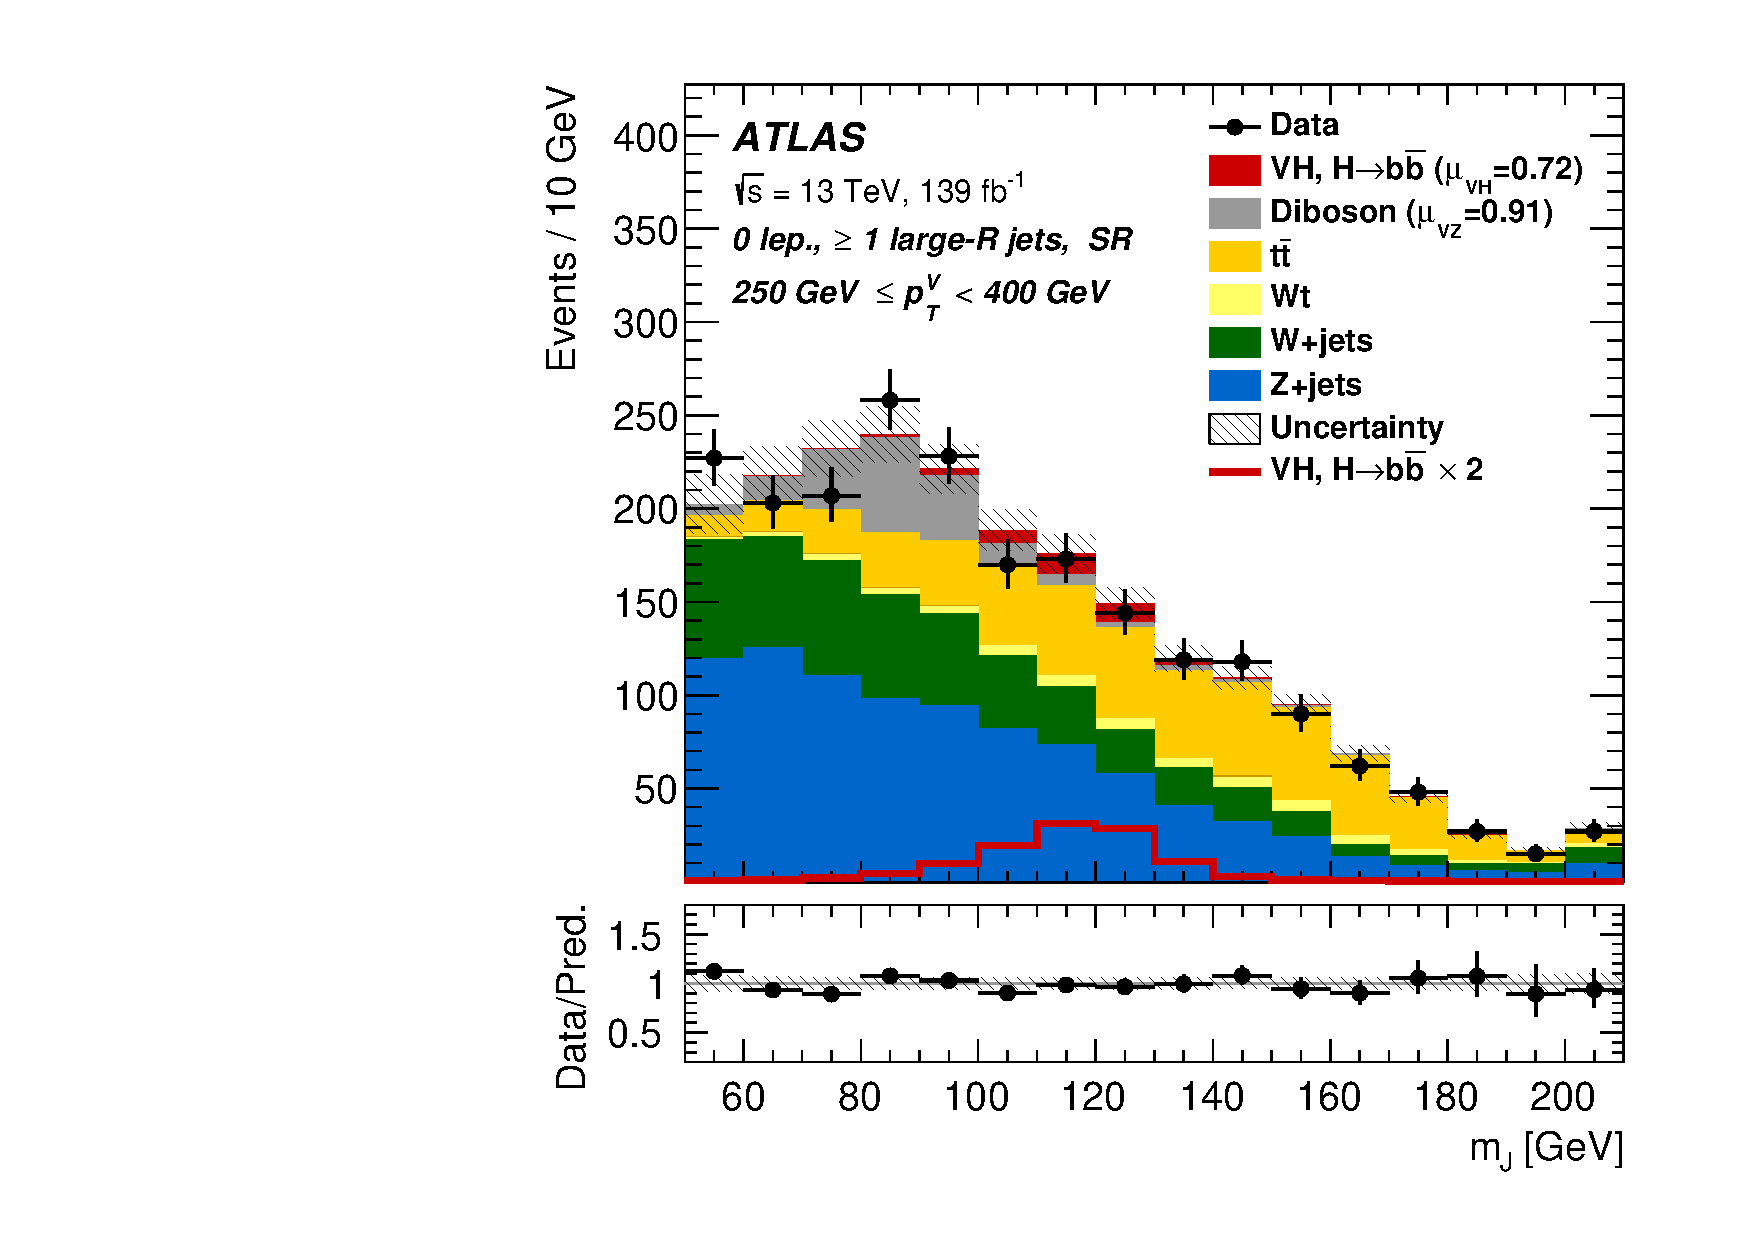
\includegraphics[width=\textwidth]{chapters/6.vhbb_boosted/figs/Region_BMin250_BMax400_incFat1_Fat1_Y6051_DSRnoaddbjetsr_T2_L0_distmBB_GlobalFit_unconditionnal_mu1.pdf}
  \end{subfigure}%
  \begin{subfigure}{.4\textwidth}
    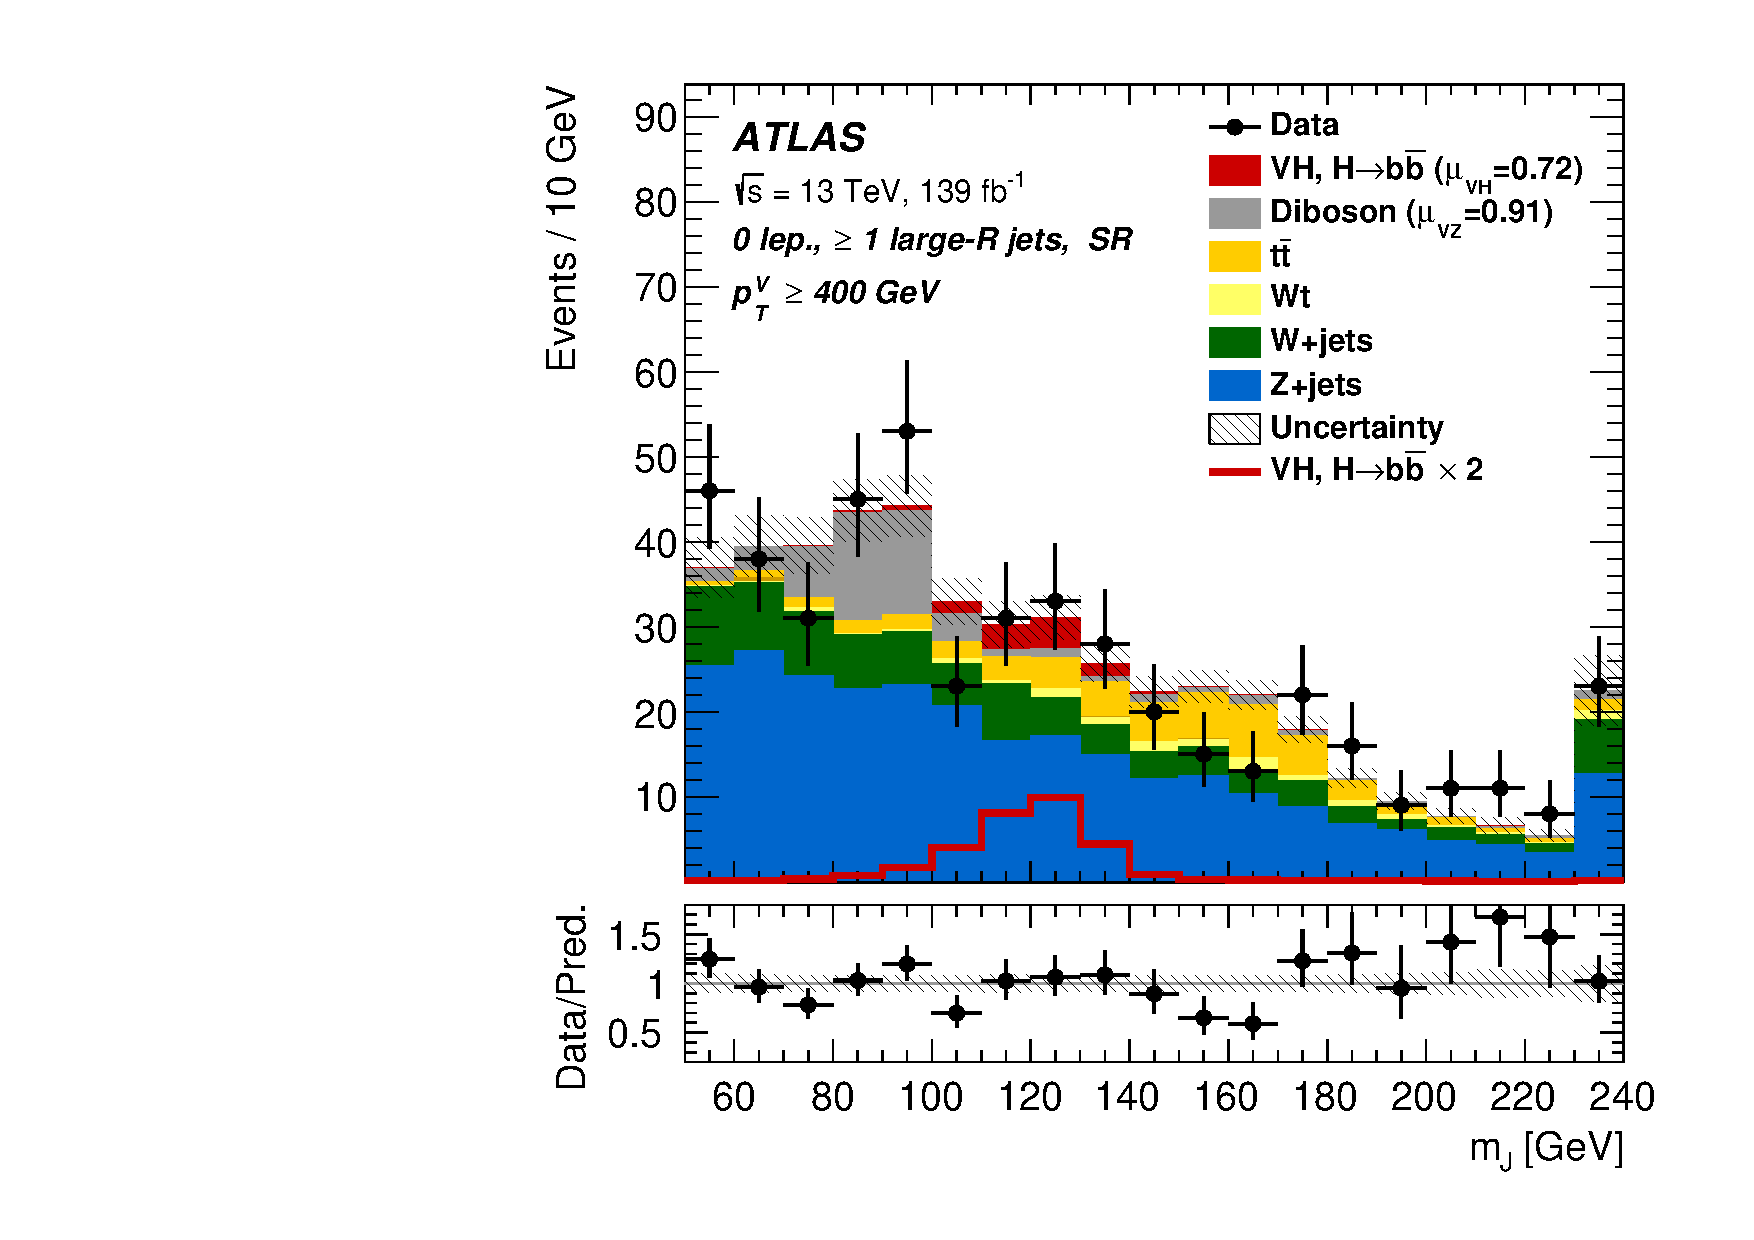
\includegraphics[width=\textwidth]{chapters/6.vhbb_boosted/figs/Region_BMin400_incFat1_Fat1_Y6051_DSRnoaddbjetsr_T2_L0_distmBB_GlobalFit_unconditionnal_mu1.pdf}
  \end{subfigure}
  \begin{subfigure}{.4\textwidth}
    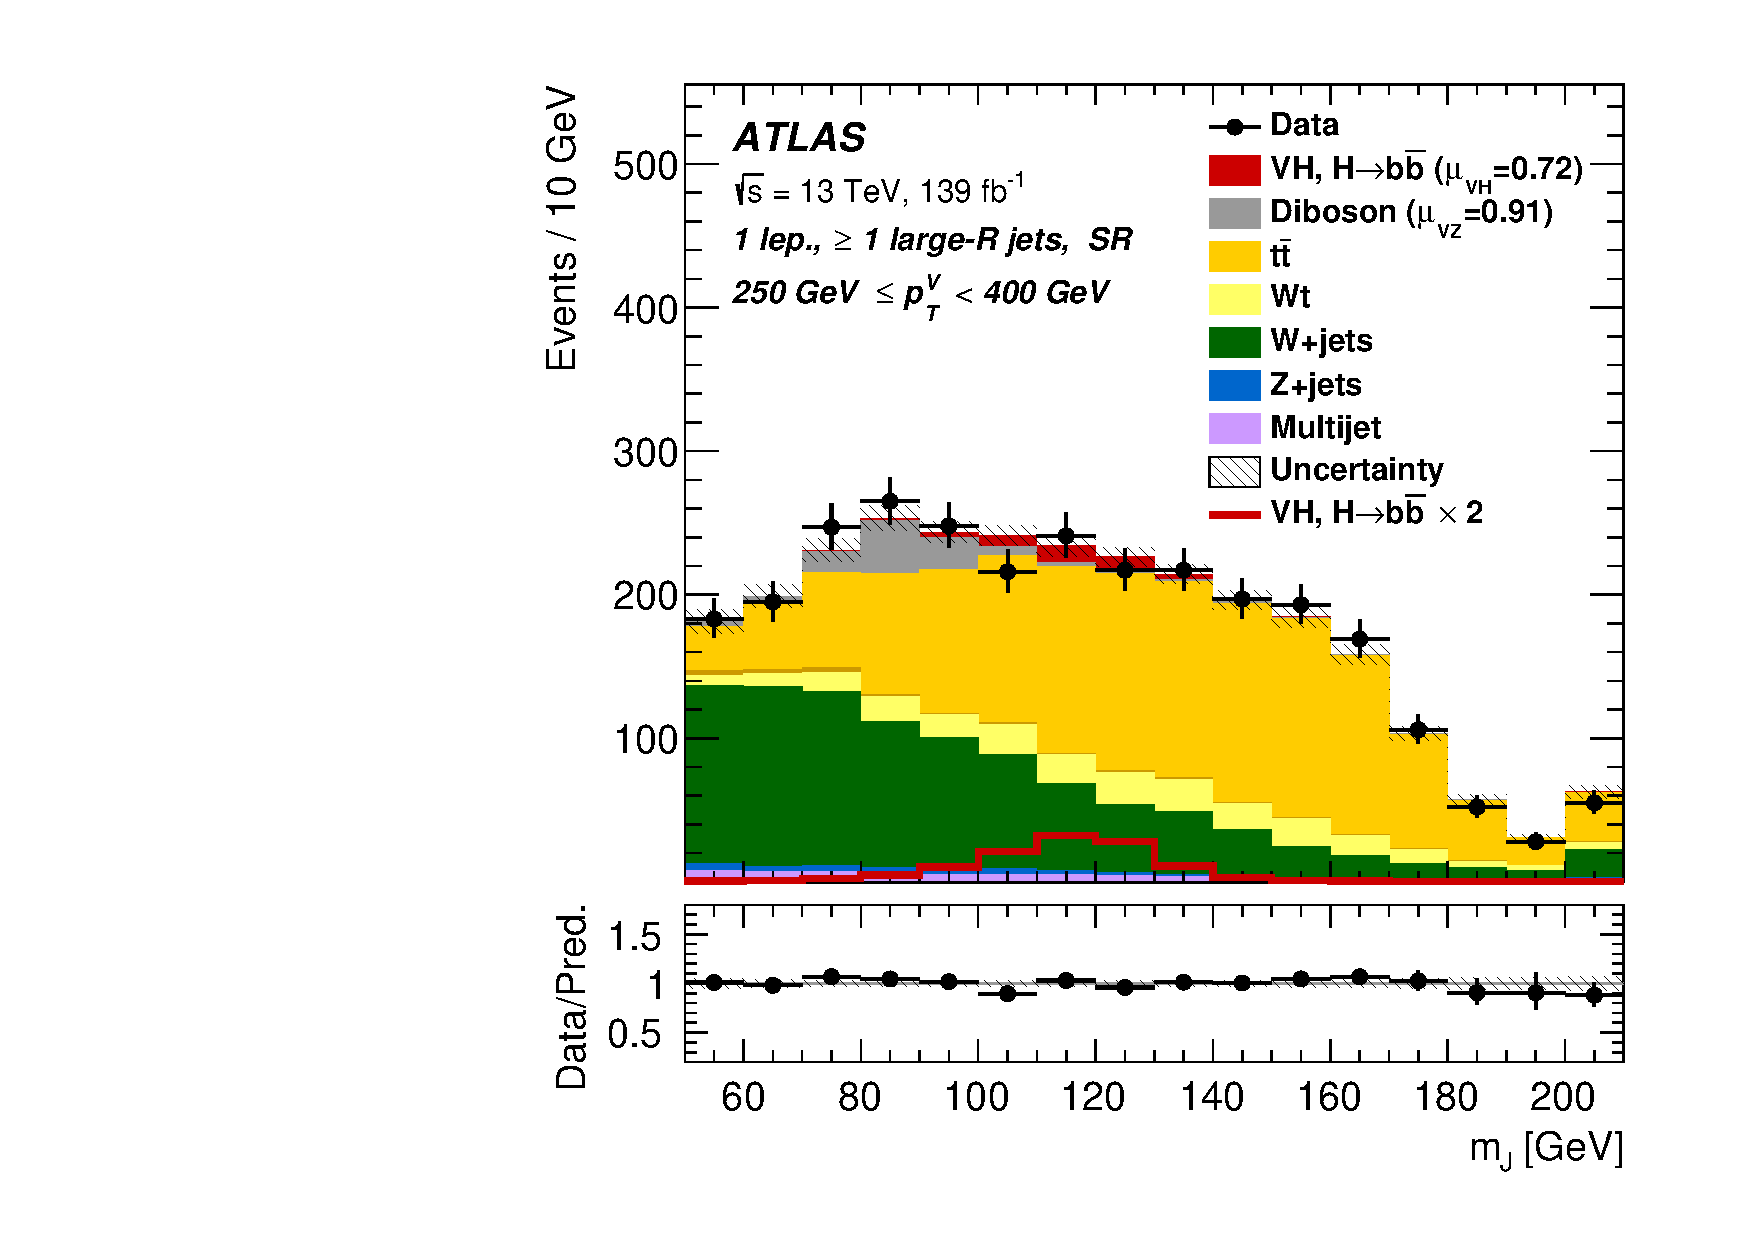
\includegraphics[width=\textwidth]{chapters/6.vhbb_boosted/figs/Region_BMin250_BMax400_incFat1_Fat1_Y6051_DSRnoaddbjetsr_T2_L1_distmBB_GlobalFit_unconditionnal_mu1.pdf}
  \end{subfigure}%
  \begin{subfigure}{.4\textwidth}
    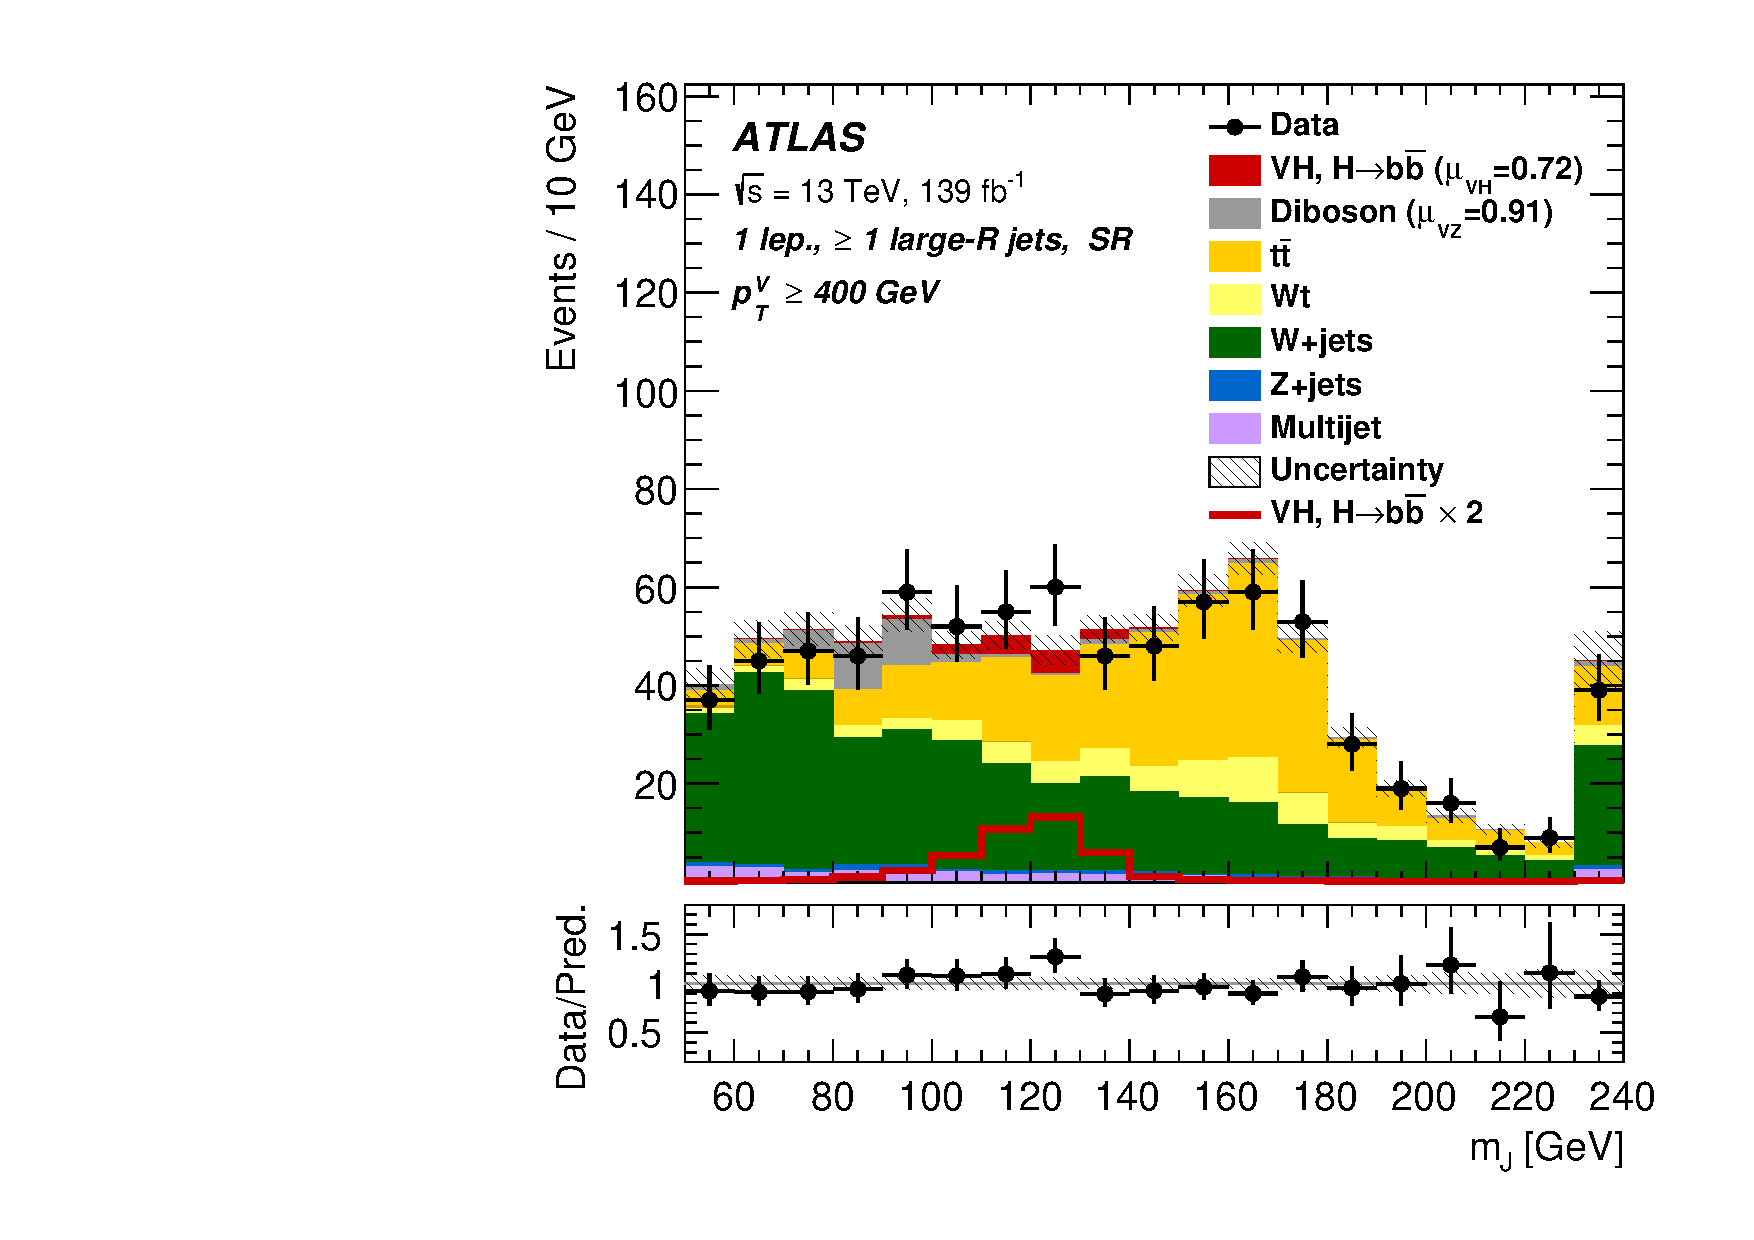
\includegraphics[width=\textwidth]{chapters/6.vhbb_boosted/figs/Region_BMin400_incFat1_Fat1_Y6051_DSRnoaddbjetsr_T2_L1_distmBB_GlobalFit_unconditionnal_mu1.pdf}
  \end{subfigure}
  \begin{subfigure}{.4\textwidth}
    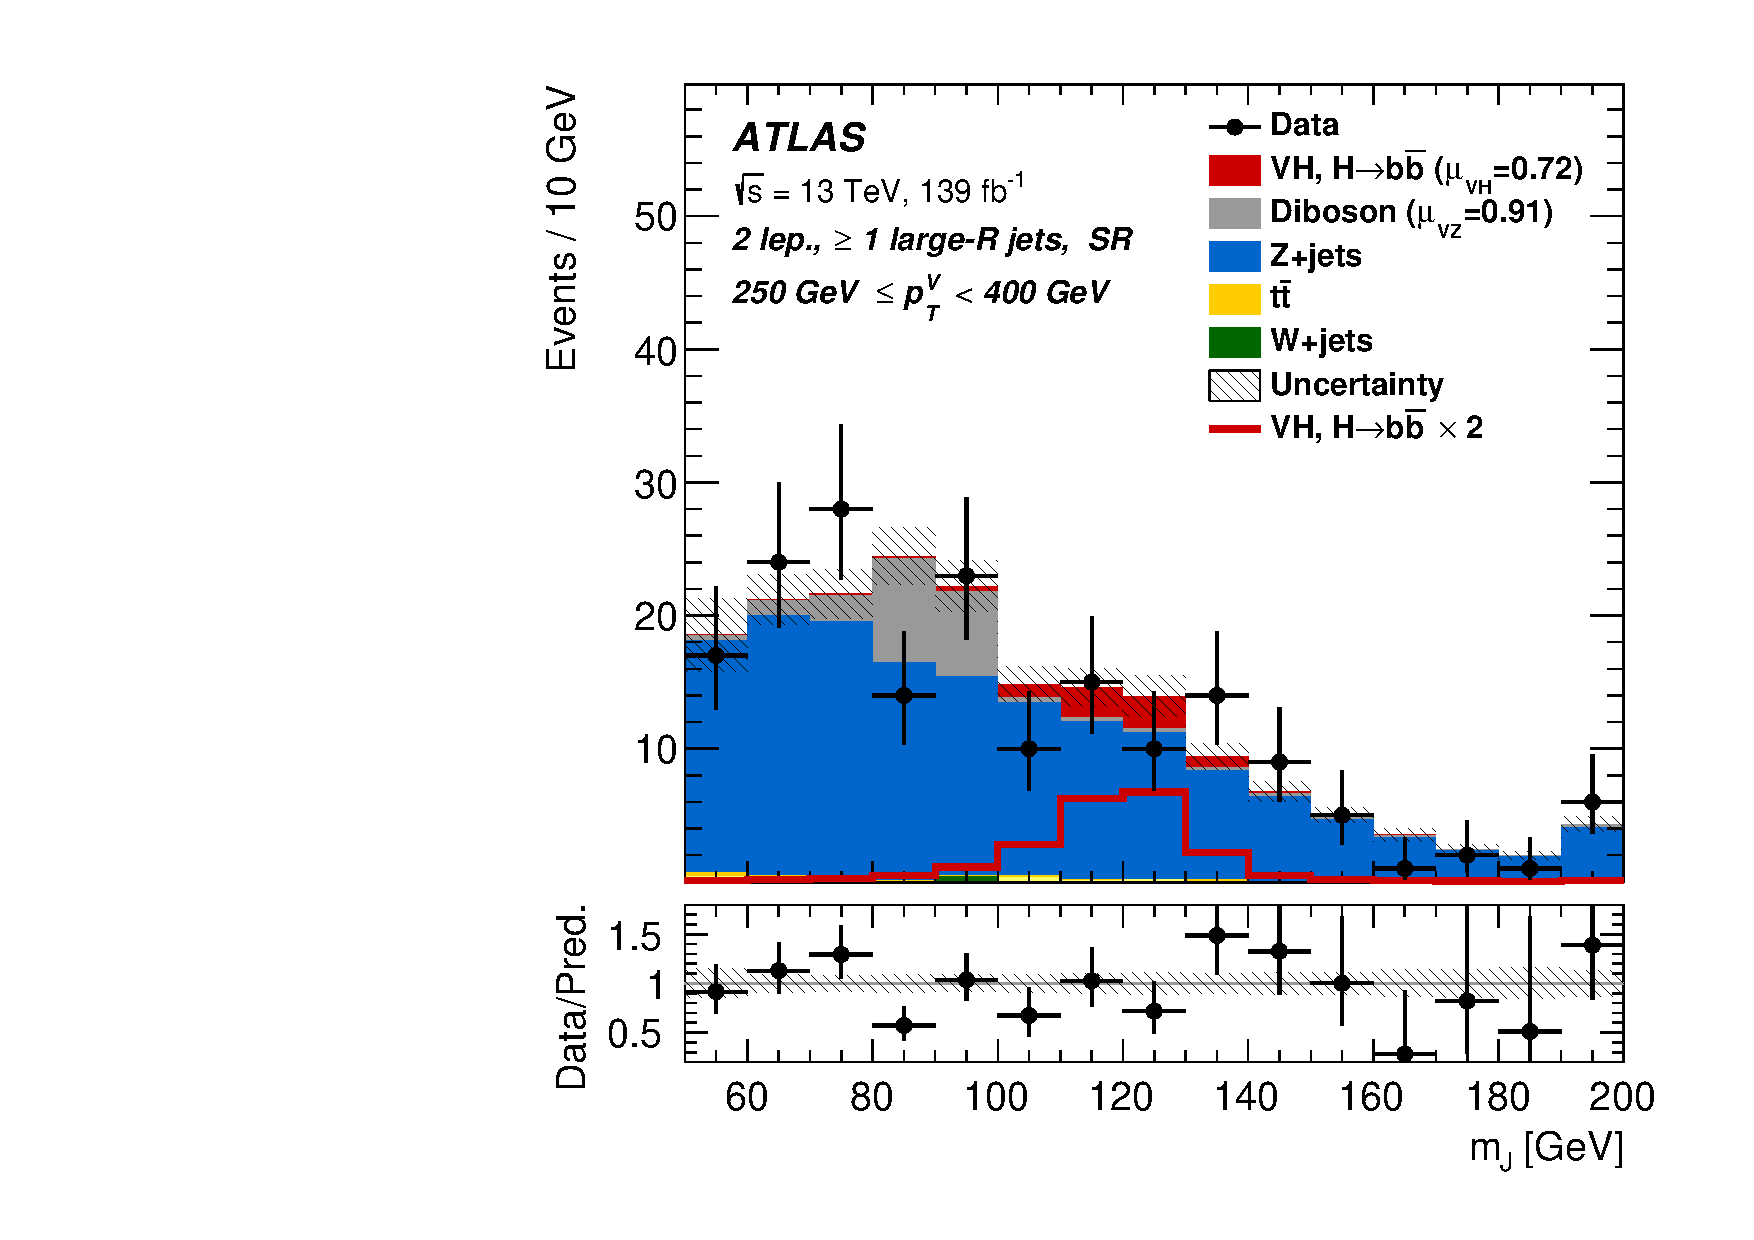
\includegraphics[width=\textwidth]{chapters/6.vhbb_boosted/figs/Region_distmBB_J0_L2_T2_DSR_Y6051_incJet1_Fat1_incFat1_BMin250_BMax400_GlobalFit_unconditionnal_mu1.pdf}
  \end{subfigure}%
  \begin{subfigure}{.4\textwidth}
    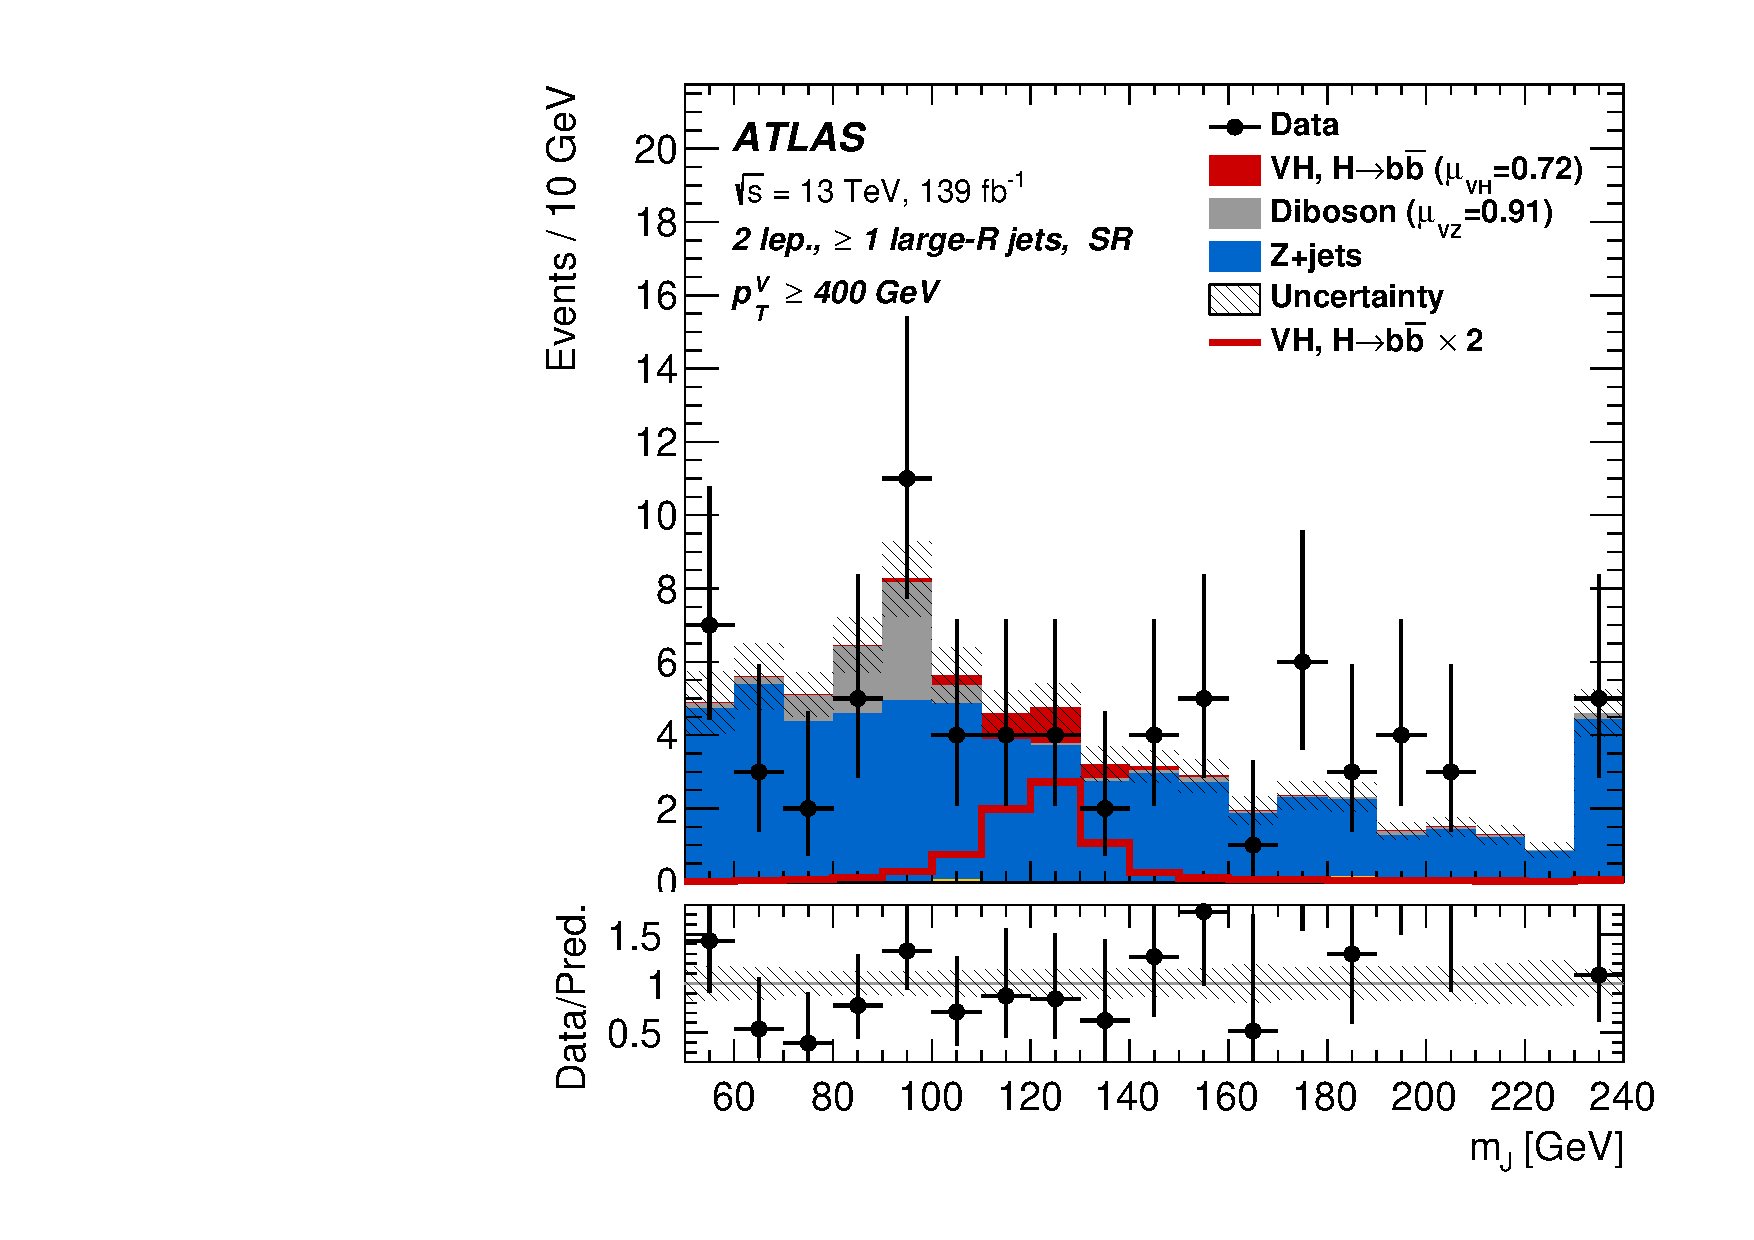
\includegraphics[width=\textwidth]{chapters/6.vhbb_boosted/figs/Region_BMin400_incFat1_Fat1_incJet1_Y6051_DSR_T2_L2_distmBB_J0_GlobalFit_unconditionnal_mu1.pdf}
  \end{subfigure}
  \caption{
    The \mJ post-fit distributions
    in (top) the 0-, (middle) 1- and (bottom) \tlep SRs for
    (left) $\SI{250}{\GeV} < \ptv < \SI{400}{\GeV}$ and (right) $\ptv \geq \SI{400}{\GeV}$ .
    The LP and HP regions are merged for the \zlep and \olep channels.
    The fitted background contributions
    are shown as filled histograms. The Higgs boson signal ($m_H =
    \SI{125}{\GeV}$) is shown as a filled histogram and is 
    normalised to the signal yield extracted from data
    ($\muVH = 0.72$), and as an unstacked unfilled histogram,
    scaled by the SM prediction times a factor of two. The size of the
    combined on the sum of the
    fitted signal and background is shown in the hatched band. The
    highest bin contains the overflow \cite{HIGG-2018-52}. 
    %The ratio of the data to the sum of the fitted signal and background is shown in the lower panel.
    %Post-fit distributions for the 0-lepton (left) and 2-lepton (right) channels in the high purity medium \pTV region, obtained in the combined conditional $\mu=1$ fit to data. The last bin of each plot is an overflow bin.
  }
  \label{fig:vhbb_postfit_plots}
\end{figure}


\begin{figure}[!htbp]
  \centering
  \begin{subfigure}{.4\textwidth}
    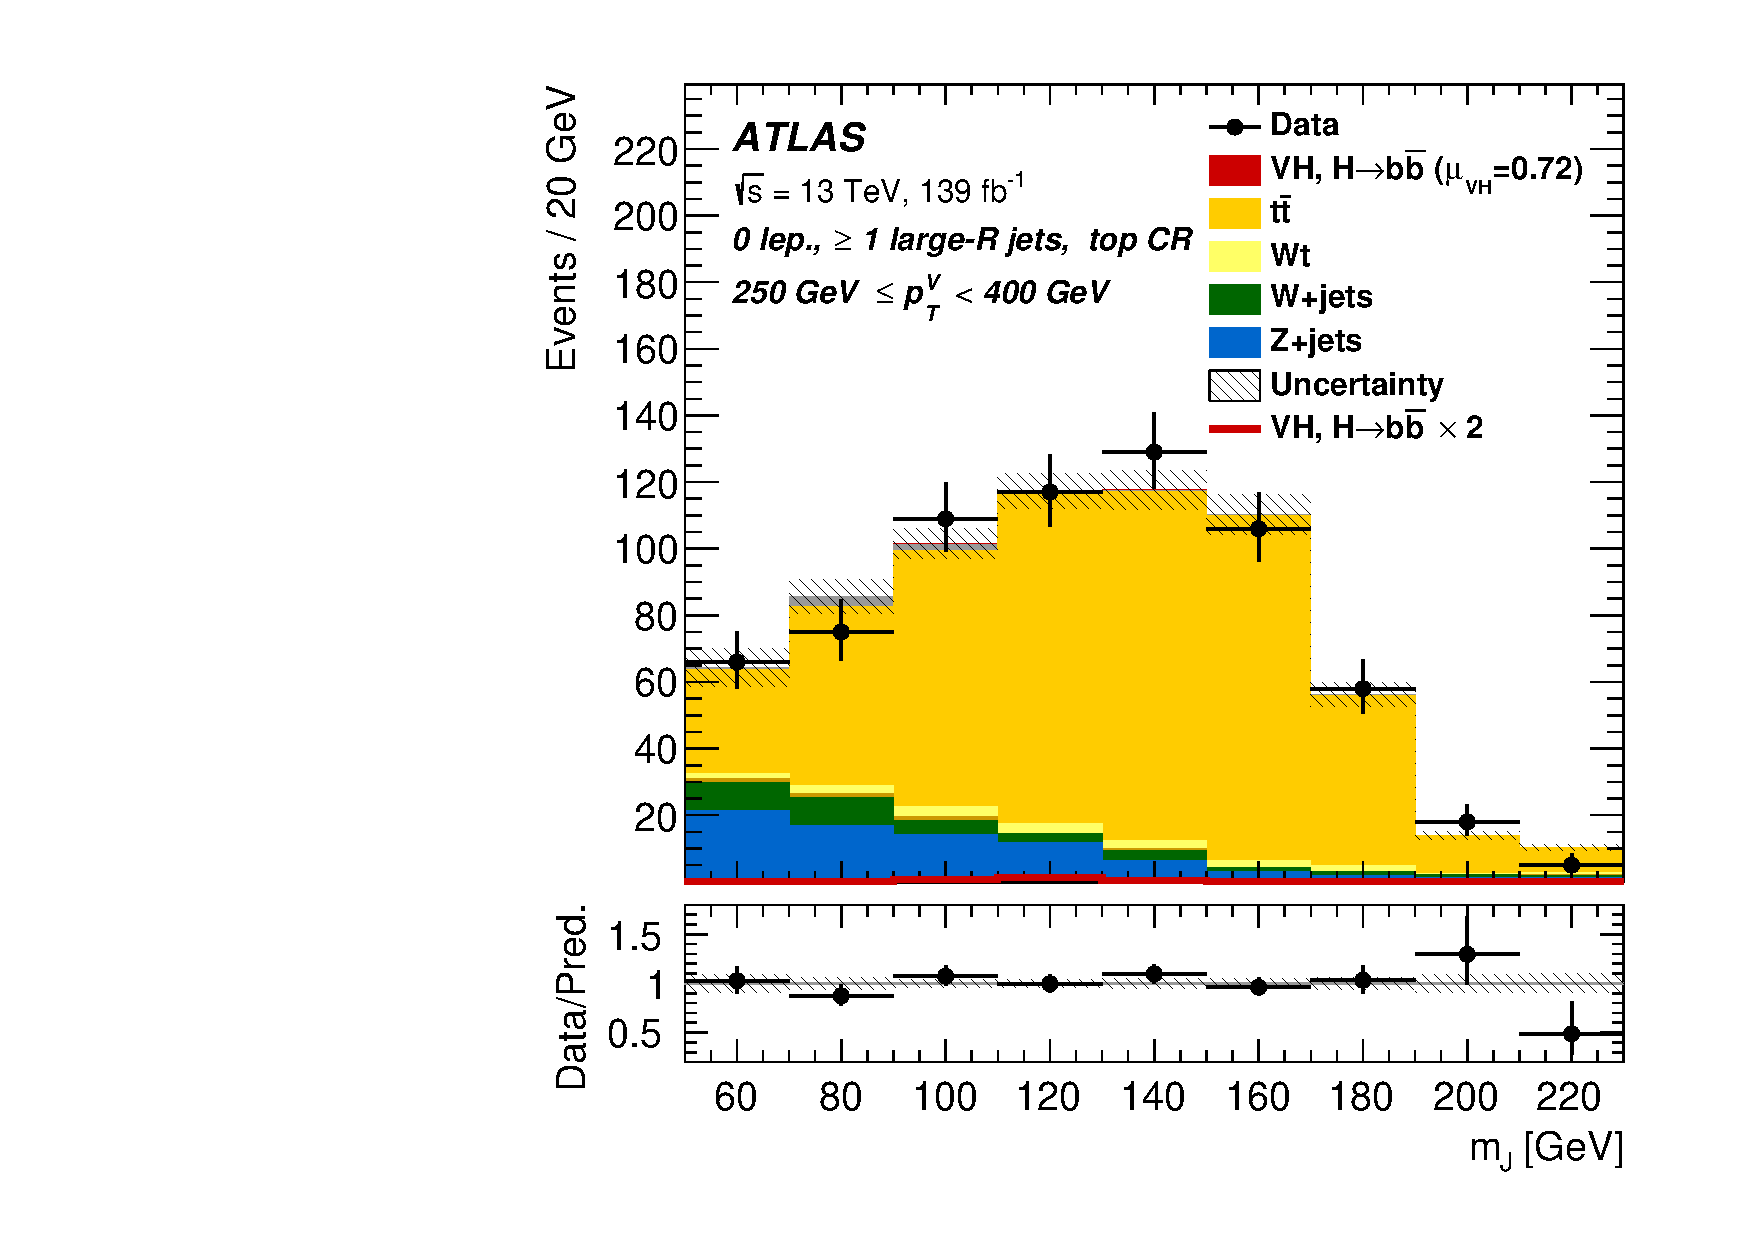
\includegraphics[width=\textwidth]{chapters/6.vhbb_boosted/figs/Region_distmBB_J0_L0_T2_DSRtopaddbjetcr_Y6051_incJet1_Fat1_incFat1_BMin250_BMax400_GlobalFit_unconditionnal_mu1.pdf}
  \end{subfigure}%
  \begin{subfigure}{.4\textwidth}
    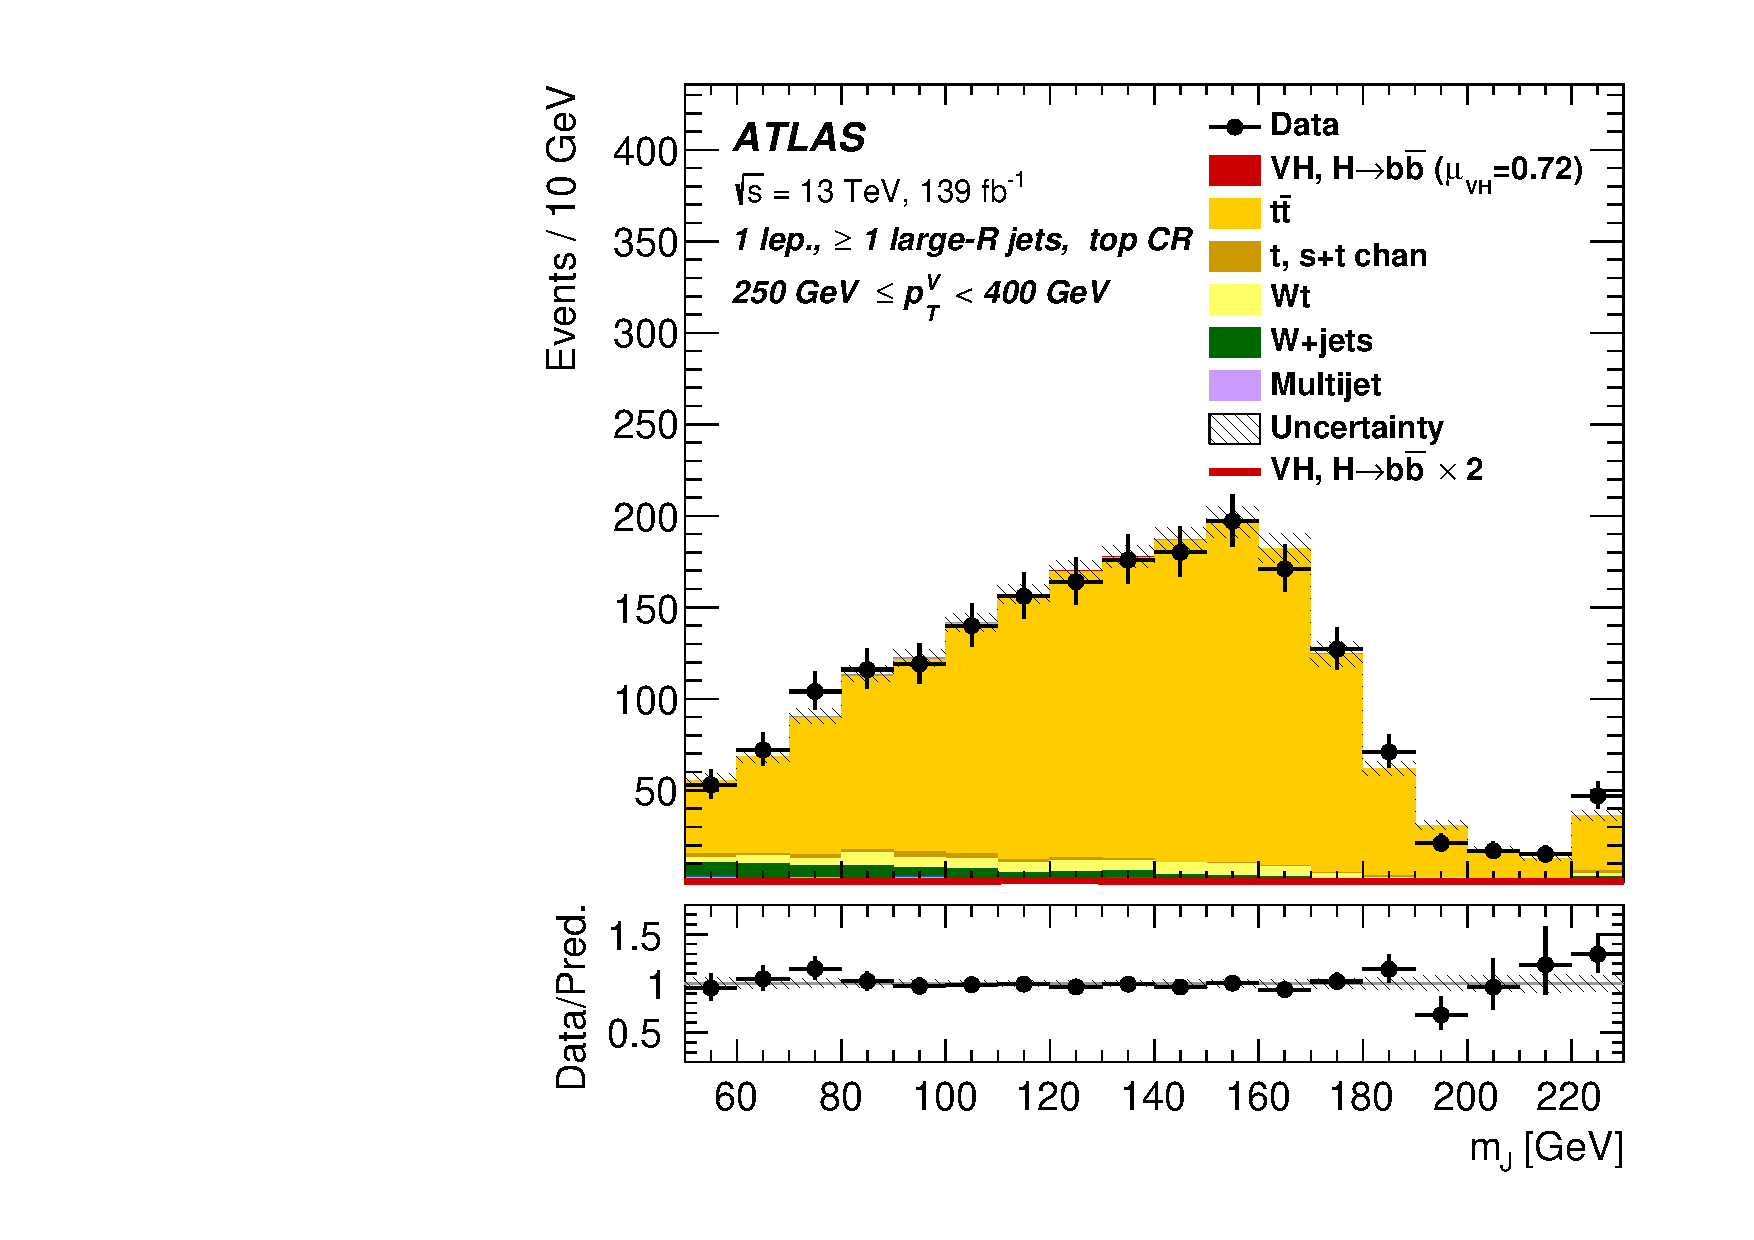
\includegraphics[width=\textwidth]{chapters/6.vhbb_boosted/figs/Region_distmBB_J0_L1_T2_DSRtopaddbjetcr_Y6051_incJet1_Fat1_incFat1_BMin250_BMax400_GlobalFit_unconditionnal_mu1.pdf}
  \end{subfigure}
  \begin{subfigure}{.4\textwidth}
    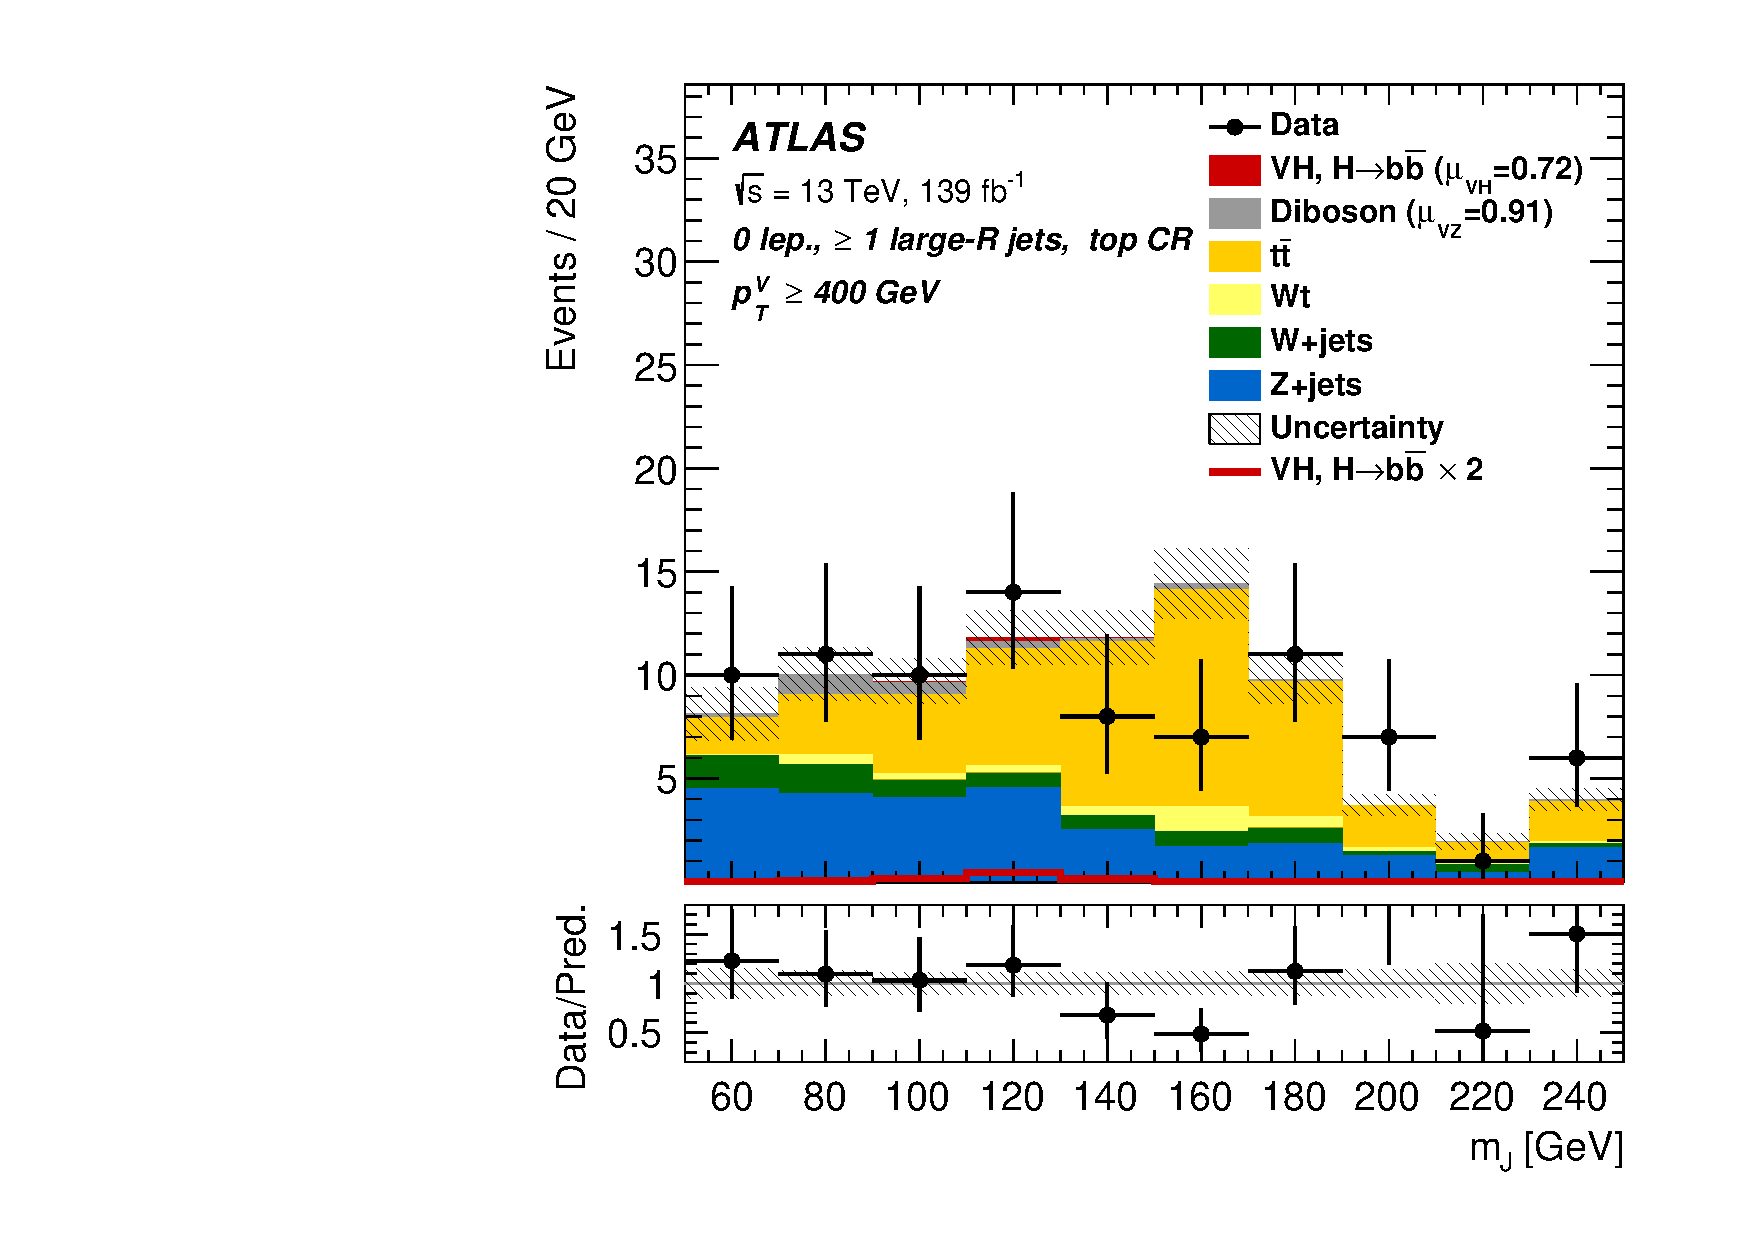
\includegraphics[width=\textwidth]{chapters/6.vhbb_boosted/figs/Region_BMin400_incFat1_Fat1_incJet1_Y6051_DSRtopaddbjetcr_T2_L0_distmBB_J0_GlobalFit_unconditionnal_mu1.pdf}
  \end{subfigure}%
  \begin{subfigure}{.4\textwidth}
    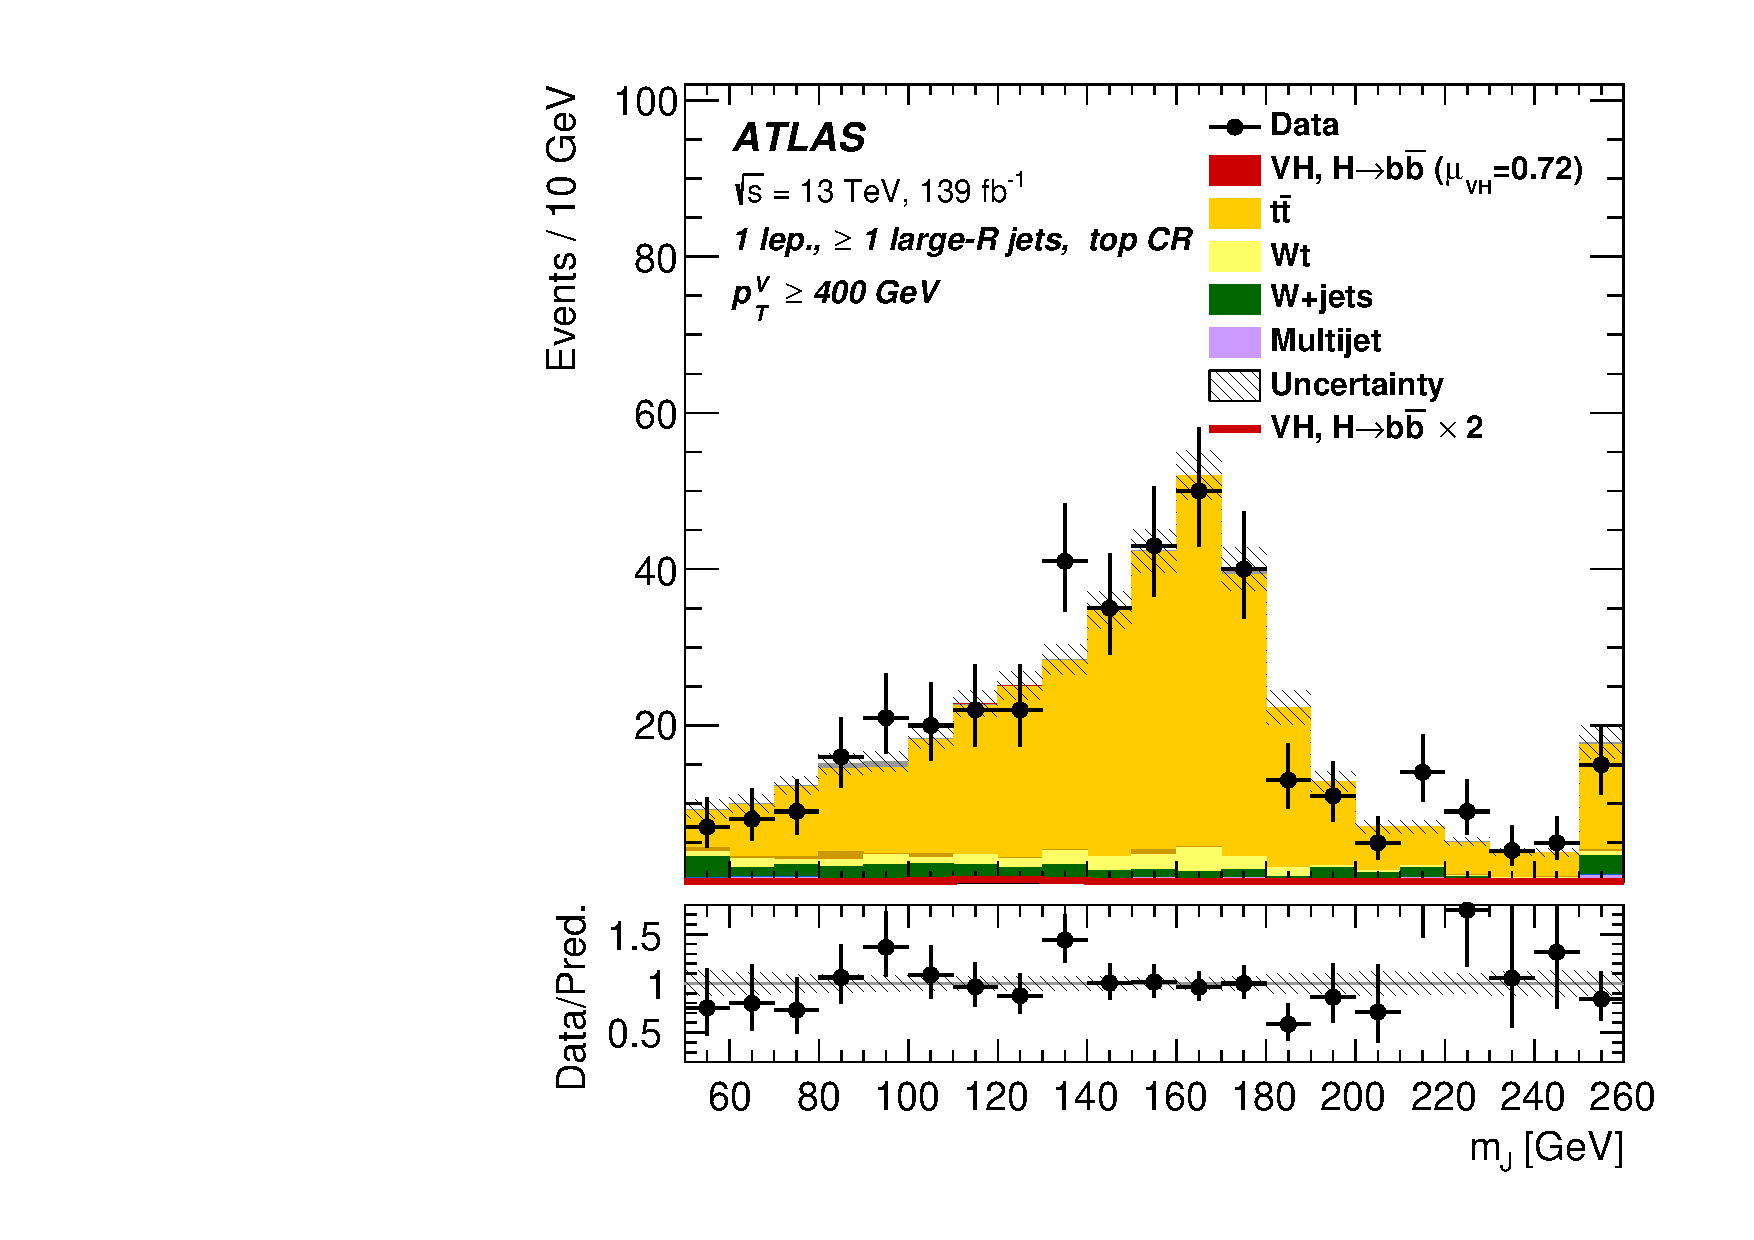
\includegraphics[width=\textwidth]{chapters/6.vhbb_boosted/figs/Region_BMin400_incFat1_Fat1_incJet1_Y6051_DSRtopaddbjetcr_T2_L1_distmBB_J0_GlobalFit_unconditionnal_mu1.pdf}
  \end{subfigure}
  \caption{
    The \mJ post-fit distributions in the \ttbar control region for
    (top) the \zlep channel and the \olep channel for $\SI{250}{\GeV} < \ptv < \SI{400}{\GeV}$
    and (bottom) the \zlep\ channel and the \olep\ channel for $\ptv > \SI{400}{\GeV}$.
    The background
    contributions after the likelihood fit are shown as filled
    histograms. The Higgs boson signal ($\mh = \SI{125}{\GeV}$) is shown as a
    filled histogram on top of the fitted backgrounds normalised to the
    signal yield extracted from data ($\mu_{VH}^{bb}=0.72$), and
    unstacked as an unfilled histogram, scaled by the SM prediction times a factor 
    of 2. The size of the combined statistical and systematic
    uncertainty for the sum of the fitted signal and background is
    indicated by the hatched band. The highest bin in the distributions
    contains the overflow \cite{HIGG-2018-52}.
  }
  \label{fig:vhbb_postfit_plots_cr}
\end{figure}




\subsection{Observed Signal Strength \& Significance}\label{sec:signal_strengh_sigs}

The measured signal strength is computed as the ratio between the measured signal yield to the prediction from the SM.
The combed result for all three lepton channels and all analysis regions is given for \muVH in \cref{eq:muVH}, and for \muVZ in \cref{eq:muVZ}.
Both results include a full breakdown of the systematic and   statistical uncertainties.
%
\begin{equation}\label{eq:muVH}
  \muVH = 0.72 ^{+0.39}_{-0.36} = 0.72 ^{+0.29}_{-0.28}  \mathrm{(stat.)} ^{+0.26}_{-0.22} \mathrm{(syst.)}
\end{equation}
%
\begin{equation}\label{eq:muVZ}
  \muVZ = 0.91 ^{+0.29}_{-0.23} = 0.91 \pm 0.15 \mathrm{(stat.)} ^{+0.24}_{-0.17} \mathrm{(syst.)} 
\end{equation}
%
The results for \muVH and \muVZ are consistent with the expectation from the SM.
The \muVH measurement is dominated by statistical uncertainty, while the \muVZ measurement is dominated by systematic sources of uncertainty.
The measured signal strength for \muVZ corresponds to an observed significance of 2.1 standard deviations, with an expected (median) significance given the SM prediction of 2.7 standard deviations.
The diboson observed (expected) signal strength significance is 5.4 (5.7).
These results are summarised in \cref{fig:money_plot}, which shows the weighted and background-subtracted \mJ distribution.
A clear signal excess is visible around the Higgs mass of $m_H = \SI{125}{\GeV}$.

\begin{figure}[!htbp]
  \centering
  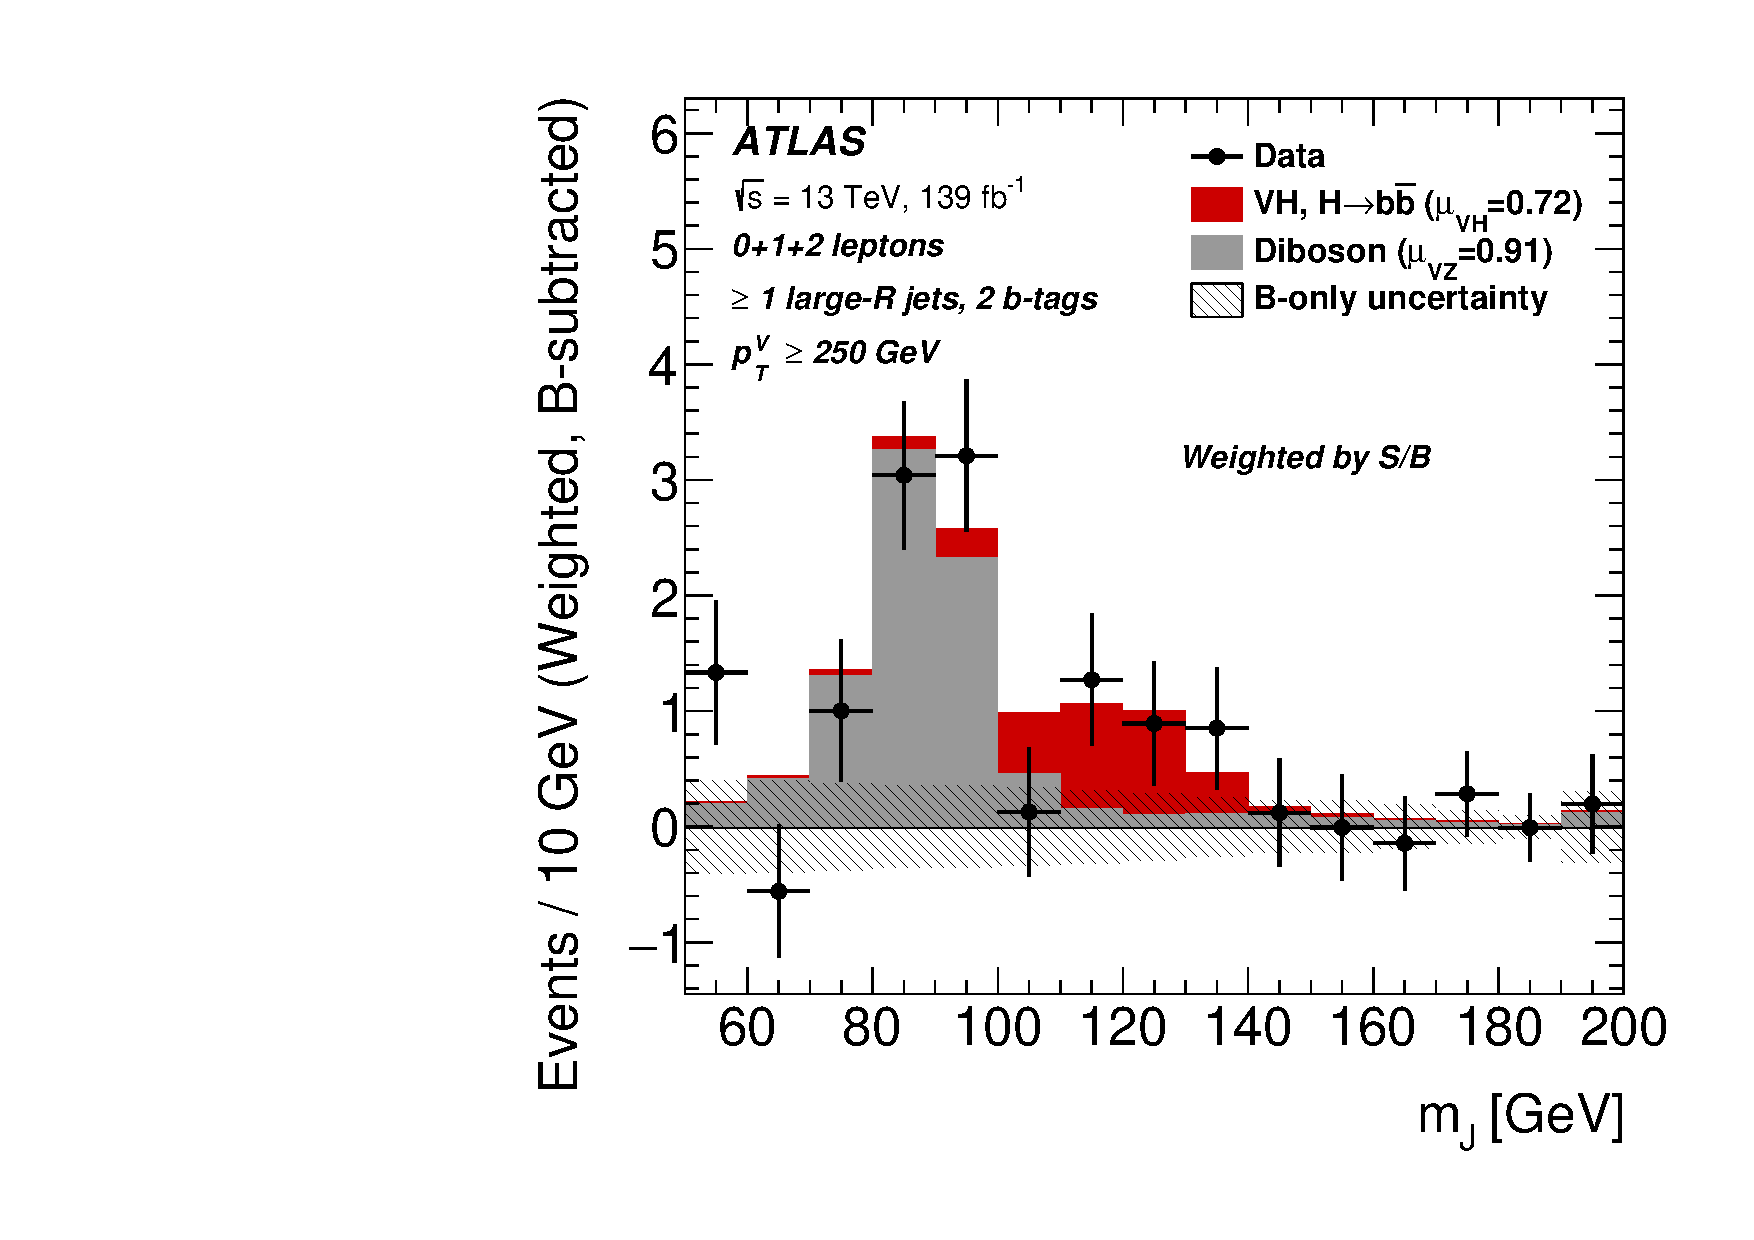
\includegraphics[width=0.7\textwidth]{chapters/6.vhbb_boosted/figs/Region_BMin250_incFat1_Fat1_incJet1_Y6051_DSRnoaddbjetsr_T2_L3_distmBB_Higgsweighted_BkgSub_GlobalFit_unconditionnal_mu1.pdf}
  \caption{
    \mJ distribution in data after subtraction of all backgrounds except for the $WZ$ and $ZZ$ diboson processes. 
    The contributions from all lepton channels and signal regions are summed and weighted by their
    respective values of the ratio of fitted Higgs boson signal and
    background yields. The expected contribution of the associated $WH$
    and $ZH$ production of a SM Higgs boson with $m_H = \SI{125}{\GeV}$ is
    shown scaled by the measured combined signal strength
    ($\muVH=0.72$). The diboson contribution is normalised to its
    best-fit value of $\muVZ=0.91$. The size of the combined
    statistical and systematic uncertainty is indicated by the hatched
    band. This error band is computed from a full signal-plus-background
    fit including all the systematic uncertainties defined in
    \cref{sec:vhbb_modelling}, except for the $VH/VZ$
    experimental and theory uncertainties  \cite{HIGG-2018-52}.  
  }
  \label{fig:money_plot}
\end{figure}

\subsubsection{Compatibility Studies}

Alongside the standard 2-POI fit, a (3+1)-POI fit can be performed by splitting \muVH into three separate POIs, one for each channel.
A simultaneous fit to the channel specific signal strengths can then be performed, which allows a comparison of the contributions from each channel.
\cref{fig:channel_comp} compares the best-fit signal strengths.
The 0- and 1-lepton channels show a signal strength which is consistent with the SM prediction, while the 2-lepton channel shows a small deviation within the $1\sigma$ uncertainty.
Overall, good compatibility is observed via a $\chi^2$ test with a corresponding $p$-value of \pct{49}.

\begin{figure}[!htbp]
  \centering
  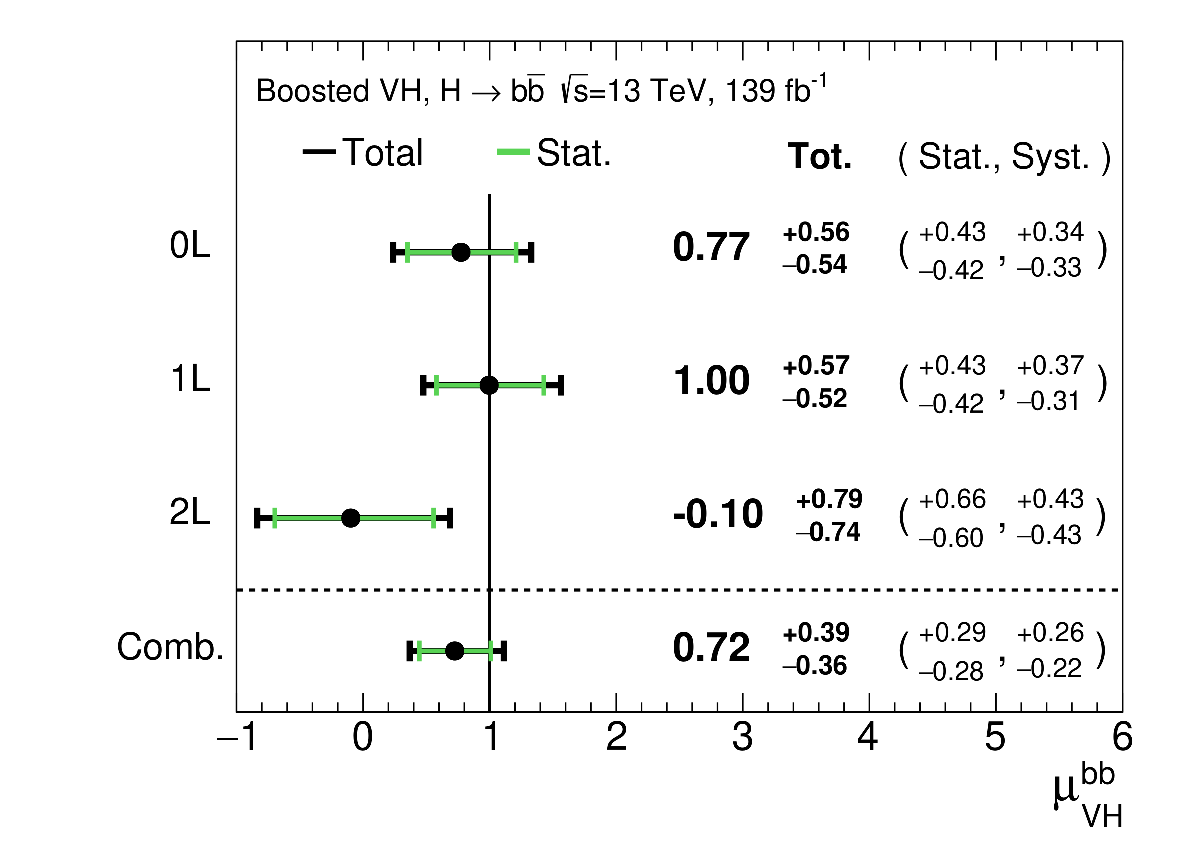
\includegraphics[width=0.7\textwidth]{chapters/6.vhbb_boosted/figs/Plot_mu_102_VH.pdf}
  \caption{
    Signal strength compatibility test between the (3+1)-POI fit (with the three lepton channels fit separately) and the default (1+1)-POI fit.
    The compatibility of the three channels is evaluated via a $\chi^2$ difference test and results in a p-value of \pct{49} \cite{HIGG-2018-52}.
  }
  \label{fig:channel_comp}
\end{figure}



\subsection{Impact of Systematics}\label{sec:sys_results}

The impact of systematic uncertainties on the final fitted value \muhatbb can be studied using the NP rankings, and the uncertainty breakdown.

\cref{fig:np_ranking} shows the NP ranking, which is used to visualise which NPs have the largest impact on the sensitivity to the fitted POI.
To obtain the ranking, a likelihood scan is performed for each NP $\theta_j$.
First, an unconditional fit is used to determine $\hat{\theta}_j$.
The NP is then fixed to its post-fit value varied by $\pm 1 \sigma$, the fit is repeated and the difference between the best-fit value of the POI, $\Delta \muhatVH$, is calculated, and used to rank the NPs.
%From this best-fit point, the NP is varied in steps and the likelihood is recomputed until the $\pm 1 \sigma_{\hat{\theta}_j}$ values are reached.
%For each corresponding value of $\theta_j$, 
In addition, the pulls and constraints for the highest ranked NPs are also shown.

The experimental uncertainty on the signal \largeR jet mass resolution (JMR) has the largest impact.
%It is a significant contributor to the overall uncertainty on \muVH in \cref{eq:muVH}.
JMR and jet energy scale (JES) uncertainties also have large impacts for the \Vjets and for the diboson backgrounds.
The freely-floating \Zhf normalisation is the second highest ranked NP, and is heavily constrained by the fit.
The $VZ$ POI \muVZ is also a significant NP when considering the primary \muVH measurement.

\begin{figure}[!htbp]
  \centering
  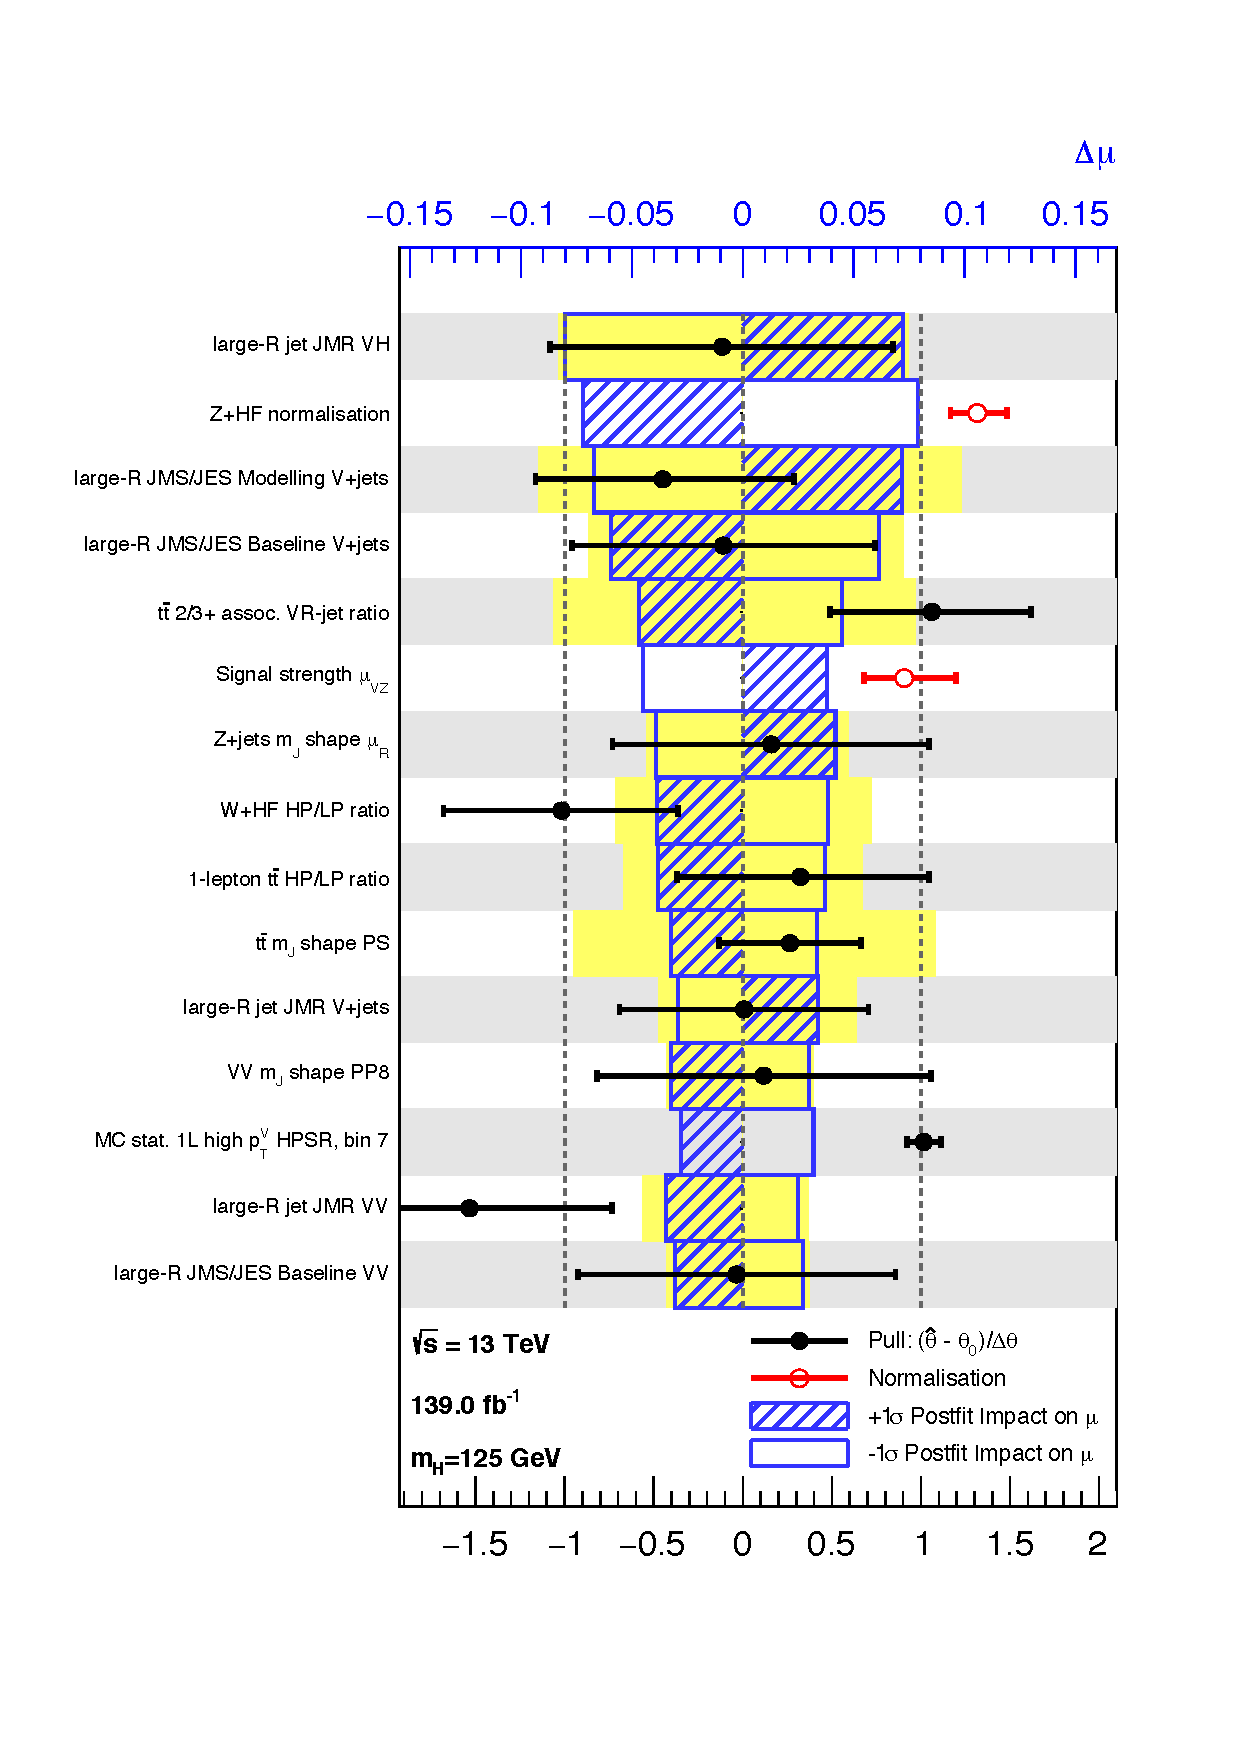
\includegraphics[width=0.7\textwidth]{chapters/6.vhbb_boosted/figs/Ranking_VH_Observed.pdf}
  \caption{
    Impact of systematic uncertainties on the fitted $VH$ signal-strength parameter \muVH sorted in decreasing order.
    The boxes show the variations of $\hat{\mu}$, referring to the top $x$-axis, when fixing the corresponding individual nuisance parameter to its post-fit value modified upwards or downwards by its post-fit uncertainty, i.e. $\hat{\theta} \pm \sigma_{\hat{\theta}}$, and repeating the fit.
    The impact of up- and down-variations can be distinguished via the dashed and plane box fillings.
    The yellow boxes show the pre-fit impact (top $x$-axis) by varying each nuisance parameter by $\pm 1$. The filled circles show the deviation of the fitted value for each nuisance parameter, $\hat{\theta}$, from their nominal input value $\theta_0$ expressed in standard deviations with respect to their nominal uncertainties $\Delta \theta$ (bottom $x$-axis).
    The error bars show the post-fit uncertainties on $\hat{\theta}$ with respect to their nominal uncertainties.
    The open circles show the fitted values and uncertainties of the normalization parameters that are freely floating in the fit.
    Pre-fit, these parameters have a value of one \cite{Dao:2688371}.
  }
  \label{fig:np_ranking}
\end{figure}

The NP ranking highlights individual NPs which have a large impact on the POI measurement sensitivity.
Complementary information is provided at a higher level by considering the overall impact of different groups of systematics.
The groups are constructed from NPs which have similar physical origins.
The impact of each group is calculated by running a fit with all the NPs in the given group fixed to their nominal values.
The uncertainty on the POI extracted from this fit is subtracted in quadrature from the uncertainty on the POI from the nominal fit, and the resulting values are provided as the impact for each group.
The total systematic impact is the difference in quadrature between the nominal uncertainty on \muVH and the estimated impact for the combined statistical uncertainties.
The ``data stat only'' group fixes all NPs at their nominal value, while the total statistical impact fixes all NPs except floating normalisations.
The floating normalisations group fixes only the NPs associated with normalisation which are left floating in the fit.

The full breakdown for the observed impact of uncertainties on the \muVH signal strength is provided in \cref{tab:mu_syst_unc}.
The uncertainty on \muVH is dominated by combined statistical effects (0.28), although the combined impact of systematics (0.24) is of a comparable size.
The signal largest group is the data stat uncertainty (0.25), demonstrating that the analysis would benefit from an increased integrated luminosity or improved efficiency to select signal events (recall from \cref{sec:vhbb_selections} the signal efficiency is in the range of \pct{10}).
Of the experimental systematic sources of uncertainty, the dominant impact is from the experimental uncertainties associated with the simulation of \largeR jets (0.13).
Other experimental sources of uncertainty are small in comparison.
Modelling uncertainties also have a large contribution to the overall systematic uncertainty.
The biggest contribution to the overall uncertainty is the combined statistical uncertainty on the simulated samples (0.09).
Out of the backgrounds, the \Wjets and \Zjets have the highest (0.06) and second-highest (0.05) impact respectively.

\begin{table}[tbp]
	\footnotesize\centering
    \setlength{\tabcolsep}{0.5em} % for the horizontal padding
    \begin{center}
    \begin{tabular}{ l | l  c c }
        \toprule\hline
        \multicolumn{2}{l}{Source of uncertainty} & Signed impact & Avg. impact \\
        \midrule
        \multicolumn{2}{l}{Total} & +0.388 / -0.356  & 0.372 \\
        \multicolumn{2}{l}{Statistical} & +0.286 / -0.280  &  0.283 \\
        \multicolumn{2}{l}{$\hookrightarrow$ Data stat only} & +0.251 / -0.245  & 0.248 \\
        \multicolumn{2}{l}{$\hookrightarrow$ Floating normalisations} & +0.096 / -0.092  & 0.094 \\
        \multicolumn{2}{l}{Systematic} & +0.261 / -0.219  & 0.240 \\
        \midrule
        \multicolumn{4}{l}{Experimental uncertainties}\\
        \midrule
        \multicolumn{2}{l}{small-R jets} &  +0.041 / -0.034  &  0.038 \\
        \multicolumn{2}{l}{large-R jets} &  +0.161 / -0.105  & 0.133 \\
        \multicolumn{2}{l}{$E_{T}^{\textrm{miss}}$} & +0.008 / -0.007  & 0.007 \\
        \multicolumn{2}{l}{Leptons} & +0.013 / -0.007  & 0.010 \\
        \multirow{3}{*}{$b$-tagging~~~} & $b$-jets & +0.028 / -0.004  & 0.016 \\
        & $c$-jets &  +0.012 / -0.011  & 0.011 \\
        & light-flavour jets & +0.009 / -0.007  & 0.008 \\
        & extrapolation & +0.004 / -0.005  & 0.004 \\
        \multicolumn{2}{l}{Pile-up} & +0.001 / -0.002  & 0.001 \\
        \multicolumn{2}{l}{Luminosity} & +0.019 / -0.007  & 0.013 \\
        \midrule
        \multicolumn{4}{l}{Theoretical and modelling uncertainties}\\
        \midrule
        \multicolumn{2}{l}{Signal} & +0.073 / -0.026  & 0.050 \\
        \multicolumn{4}{l}{} \\
        \multicolumn{2}{l}{Backgrounds} & +0.106 / -0.095  & 0.100 \\
        \multicolumn{2}{l}{$\hookrightarrow$ $Z$~+~jets} & +0.049 / -0.047  & 0.048 \\
        \multicolumn{2}{l}{$\hookrightarrow$ $W$~+~jets} & +0.059 / -0.056  & 0.058 \\
        \multicolumn{2}{l}{$\hookrightarrow$ $t\bar{t}$} & +0.037 / -0.032  & 0.035 \\
        \multicolumn{2}{l}{$\hookrightarrow$ Single top quark} & +0.031 / -0.023  & 0.027 \\
        \multicolumn{2}{l}{$\hookrightarrow$ Diboson} & +0.034 / -0.029  & 0.032 \\
        \multicolumn{2}{l}{$\hookrightarrow$ Multijet} & +0.009 / -0.009  & 0.009 \\
        \multicolumn{2}{l}{$\hookrightarrow$ MC statistical} & +0.091 / -0.092  & 0.092 \\        
        \hline\bottomrule
    \end{tabular}
    \end{center}
    \caption{
        Breakdown of the absolute contributions to the uncertainty on the signal strength $\mu_{VH}^{bb}$ obtained from the (1+1)-POI fit. 
        The average impact represents the average between the positive and negative uncertainties on $\mu_{VH}^{bb}$.
        The sum in quadrature of the systematic uncertainties attached to the categories differs from the total systematic uncertainty due to correlations \cite{Dao:2688371}. 
    }
    \label{tab:mu_syst_unc}
\end{table}
    

\subsection{STXS Interpretation}\label{sec:stxs}

The Simplified Template Cross Sections (STXS) framework provides a common categorisation of candidate Higgs boson events according to certain truth-level properties of the production mode under study \cite{deFlorian:2016spz,Badger:2016bpw}.
The STXS framework is designed to be independent of the decay mode of the Higgs boson, and is therefore well suited to the combination of measurements between different decay channels and experiments.

The STXS cross sections are independently measured for the $ZH$ and $WH$ production modes following the approach described in \cite{HIGG-2018-50}.
For each production mode, two bins in the truth vector boson transverse momentum $p_\textrm{T}^{V,t}$ are considered, $\SI{250}{\GeV} < p_\textrm{T}^{V,t} < \SI{400}{\GeV}$ and $p_\textrm{T}^{V,t} \geq \SI{400}{\GeV}$, leading to four independent analysis regions.
Events from the simulated signal samples are categorised into the regions and used to estimate the expected cross section times branching ratio $\sigma \times B$ in each region, where
%
\begin{equation}
  B =  B(\Hbb) \times B(V \rightarrow \text{leptons}),
\end{equation}
%
A simultaneous fit of the four cross section times branching ratios is performed.
The uncertainties described in \cref{sec:vhbb_modelling} are reused for the STXS fit, with the exception of the theoretical uncertainties on the signal cross section and branching ratios.
The result from the fit is shown in \cref{fig:STXSBinXSPlot} and compared with the expected prediction from the SM.
The expected and observed results agree within the given uncertainties.


\begin{figure}[!htbp]
  \centering
  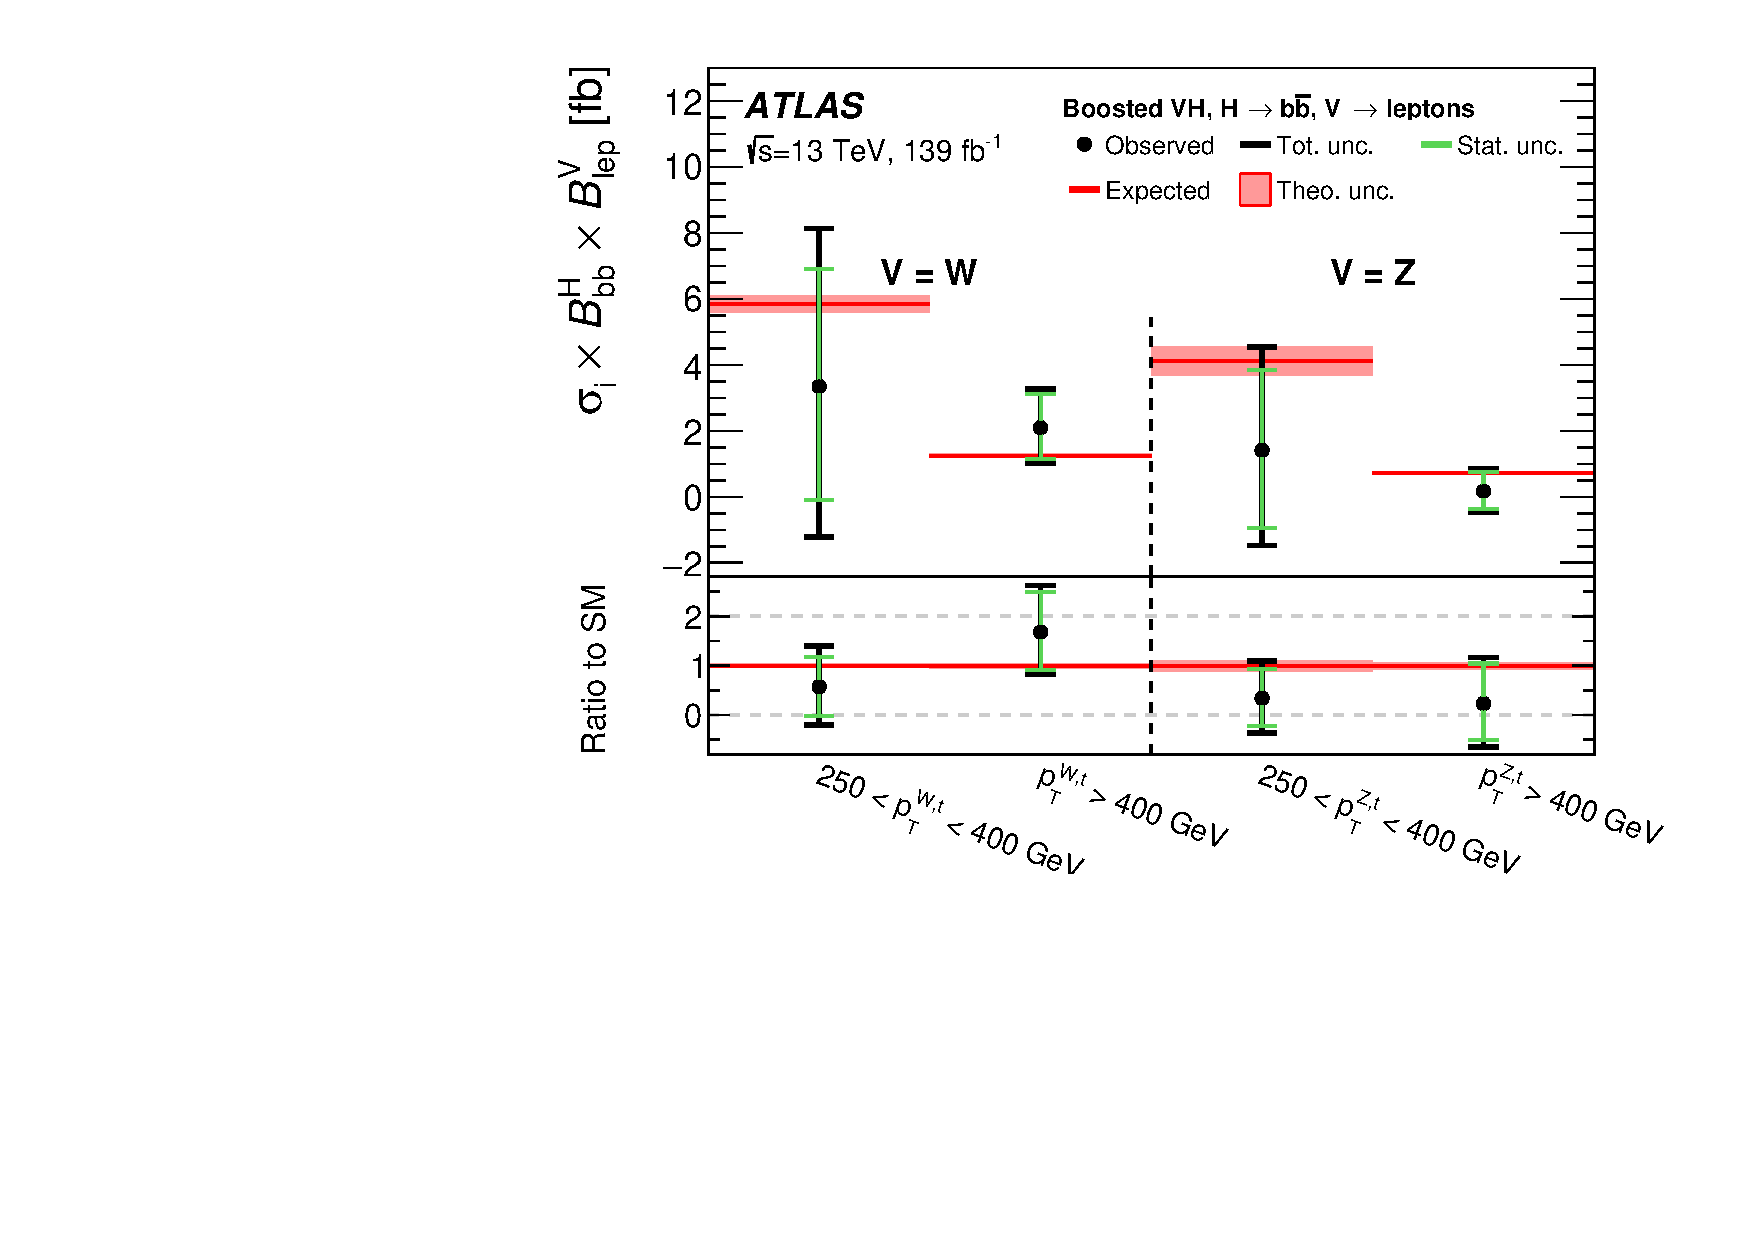
\includegraphics[width=0.7\textwidth]{chapters/6.vhbb_boosted/figs/C_STXS_XS_Atlas.pdf}
  \label{fig:STXSBinXSPlot}
  \caption{
    Measured $VH$ simplified template cross sections times the $H \rightarrow \bbbar$ and $V \rightarrow$~leptons branching fractions in the medium and high $p_\textrm{T}^{V,t}$ bins~\cite{HIGG-2018-52}.
  }
\end{figure}


\section{Conclusion}

The analysis of the associated production of vector bosons with boosted Higgs bosons decaying to a pair of \bquarks using \largeR jets is presented.
The Higgs candidate is reconstructed as a \largeR jet in order to improve sensitivity in the boosted regime in which the Higgs decay products are significantly collimated.
The analysis is performed using \intlumi of proton--proton collision data at \come{13} collected throughout the duration of \runtwo of the \LHC.

In comparison with the null hypothesis, the Standard Model (SM) \VHbb process is found to have an observed significance of $2.1$ standard deviations, whereas the corresponding expected significance is $2.7$ standard deviations.
The \VHbb process is measured simultaneously with the diboson \VZbb process, which provide a cross-check for the main analysis. 
The observed (expected) significance for the diboson process is $5.4$ ($5.7$).

The results are interpreted in the context of the STXS framework.
The cross sections for the $WH$ and $ZH$ processes are measured in two \ptv bins, and are found to agree with the SM prediction within the given uncertainties.
At the time of publication, the results are the most precise measurements of the $WH$ and $ZH$, \Hbb cross sections in the high \ptv regime.

The statistical and systematic sources of uncertainty contribute a similar amount to the overall uncertainty on the result.
This analysis would therefore likely benefit greatly from the improved \btagging efficiency at \highpt enabled by \GNN as discussed in \cref{chap:gnn_tagger}, due to the associated reduction in statistical uncertainty provided by the increased number of events used in the analysis.

The \largeR jet mass resolution is found to be the dominant source of systematic uncertainty on the \muVH measurement.
An improved method of reconstructing the \largeR jet mass, for example by using a machine learning based regression approach, possibly as an 
additional auxiliary task to \GNN (see \cref{chap:gnn_tagger}), could reduce the systematic uncertainty on the \muVH measurement.
Statistical uncertainty could be reduced by increasing the integrated luminosity used to perform the analysis by combining with \runthree data.
